%%%%%%%%%%%%%%%%%%%%%%%%%%%%%%%%%%%%%%%%%
% Classicthesis Typographic Thesis
% LaTeX Template
% Version 1.1 (4/8/12)
%
% This template has been downloaded from:
% http://www.LaTeXTemplates.com
%
% Original author:
% André Miede (http://www.miede.de)
%
% License:
% CC BY-NC-SA 3.0 (http://creativecommons.org/licenses/by-nc-sa/3.0/)
%
% General Tips:
% 1) Make sure to edit the classicthesis-config.file
% 2) New enumeration (A., B., C., etc in small caps): \begin{aenumerate} \end{aenumerate}
% 3) For margin notes: \marginpar or \graffito{}
% 4) Do not use bold fonts in this style, it is designed around them
% 5) Use tables as in the examples
% 6) See classicthesis-preamble.sty for useful commands
%
%%%%%%%%%%%%%%%%%%%%%%%%%%%%%%%%%%%%%%%%%

%----------------------------------------------------------------------------------------
%	PACKAGES AND OTHER DOCUMENT CONFIGURATIONS
%----------------------------------------------------------------------------------------

\documentclass[
	 oneside,openright,titlepage,numbers=noenddot,headinclude,%1headlines,
                footinclude=true,cleardoublepage=empty,
                BCOR=0mm,paper=a4,fontsize=11pt, % Binding correction, paper type and font size
                american, % Languages
                ]{scrreprt} 
                
% Includes the file which contains all the document configurations and packages - make sure to edit this file
%%%%%%%%%%%%%%%%%%%%%%%%%%%%%%%%%%%%%%%%%
% Thesis Configuration File
%
% The main lines to change in this file are in the DOCUMENT VARIABLES
% section, the rest of the file is for advanced configuration.
%
%%%%%%%%%%%%%%%%%%%%%%%%%%%%%%%%%%%%%%%%%

%----------------------------------------------------------------------------------------
%	DOCUMENT VARIABLES
%	Fill in the lines below to enter your information into the thesis template
%	Each of the commands can be cited anywhere in the thesis
%----------------------------------------------------------------------------------------

% Remove drafting to get rid of the '[ Date - classicthesis version 4.0 ]' text at the bottom of every page
\PassOptionsToPackage{eulerchapternumbers,listings, pdfspacing, dottedtoc, subfig,beramono,eulermath,parts, floatperchapter}{classicthesis}
% Available options: drafting parts nochapters linedheaders eulerchapternumbers beramono eulermath pdfspacing minionprospacing tocaligned dottedtoc manychapters listings floatperchapter subfig
% Adding 'dottedtoc' will make page numbers in the table of contents flushed right with dots leading to them


\usepackage{xspace} % To get the spacing after macros right


\newcommand{\myTitle}{Modeling the role of different cell types \protect\\ in development and encoding of visual statistics \protect\\ in the primary visual cortex\xspace}
\newcommand{\mySubtitle}{\xspace}
\newcommand{\myDegree}{Doctor of Philosophy\xspace}
\newcommand{\myName}{Philipp John Frederic Rudiger\xspace}
\newcommand{\myProf}{Dr. James Bednar\xspace}
\newcommand{\myOtherProf}{Dr. Alexander Thiele\xspace}
\newcommand{\mySupervisor}{Dr. James Bednar\xspace}
\newcommand{\myFaculty}{Institute of Adaptive and Neural Computation\xspace}
\newcommand{\myDepartment}{School of Informatics\xspace}
\newcommand{\myUni}{University of Edinburgh\xspace}
\newcommand{\myLocation}{Edinburgh\xspace}
\newcommand{\myTime}{2016\xspace}
\newcommand{\myVersion}{version 4.0\xspace}

%----------------------------------------------------------------------------------------
%	USEFUL COMMANDS
%----------------------------------------------------------------------------------------

\newcommand{\ie}{i.\,e.}
\newcommand{\Ie}{I.\,e.}
\newcommand{\eg}{e.\,g.}
\newcommand{\Eg}{E.\,g.} 
\newcommand{\mm}[0]{$\mathrm{\mu m}$ }
%\newcommand{\degree}{\ensuremath{^\circ}}
\newcommand{\ih}[0]{$I_{h}$ }
\newcommand{\cm}[0]{$cm^{2}$}
\newcommand{\lyxdot}{.}
\newcommand{\sq}[0]{$^{2}$ }

\newcounter{dummy} % Necessary for correct hyperlinks (to index, bib, etc.)
\providecommand{\mLyX}{L\kern-.1667em\lower.25em\hbox{Y}\kern-.125emX\@}

\usepackage{mathtools}
\DeclarePairedDelimiter{\abs}{\lvert}{\rvert}


%----------------------------------------------------------------------------------------
%	PACKAGES
%----------------------------------------------------------------------------------------

\usepackage[dvipsnames]{xcolor}
\usepackage{siunitx}
\usepackage{mathtools}
\usepackage{gensymb}
\usepackage{amssymb}
\usepackage{graphicx}
\usepackage{wasysym}
\usepackage{adjustbox}
\usepackage[utf8x]{inputenc}
\usepackage{pdfpages}


%------------------------------------------------
 
\PassOptionsToPackage{utf8}{inputenc} % latin9 (ISO-8859-9) = latin1+"Euro sign"
\usepackage{inputenc}
 
 %------------------------------------------------

%\PassOptionsToPackage{ngerman,american}{babel}  % Change this to your language(s)
% Spanish languages need extra options in order to work with this template
%\PassOptionsToPackage{spanish,es-lcroman}{babel}
\usepackage[english]{babel}

%------------------------------------------------			

%\PassOptionsToPackage{square,numbers}{natbib}
\usepackage{natbib, natbibspacing}
%% \usepackage[warnundef]{jabbrv} % changed HR 26/5/13

 
 %------------------------------------------------

\PassOptionsToPackage{fleqn}{amsmath} % Math environments and more by the AMS 
 \usepackage{amsmath}
 
 %------------------------------------------------

\PassOptionsToPackage{T1}{fontenc} % T2A for cyrillics
\usepackage{fontenc}

%------------------------------------------------

%------------------------------------------------

\usepackage{mparhack} % To get marginpar right

%------------------------------------------------

\usepackage{fixltx2e} % Fixes some LaTeX stuff 

%------------------------------------------------

\PassOptionsToPackage{smaller}{acronym} % Include printonlyused in the first bracket to only show acronyms used in the text
\usepackage{acronym} % nice macros for handling all acronyms in the thesis

%------------------------------------------------

%\renewcommand*{\acsfont}[1]{\textssc{#1}} % For MinionPro
\newcommand{\bflabel}[1]{{#1}\hfill} % Fix the list of acronyms

%------------------------------------------------

\PassOptionsToPackage{pdftex}{graphicx}
\usepackage{graphicx} 

\usepackage{gensymb}

\usepackage{mhchem}

\usepackage{pdflscape}

\usepackage{rotating}

\usepackage{color}
\usepackage{booktabs}
\usepackage{array}
\usepackage{grffile}
\usepackage{longtable}
\usepackage{keyval}
\usepackage{verbatim}
\usepackage{setspace}
\usepackage{framed,color}
\definecolor{shadecolor}{gray}{0.9}
%\usepackage{bibspacing}
%----------------------------------------------------------------------------------------
%	FLOATS: TABLES, FIGURES AND CAPTIONS SETUP
%----------------------------------------------------------------------------------------

\usepackage{tabularx} % Better tables
\setlength{\extrarowheight}{3pt} % Increase table row height
\newcommand{\tableheadline}[1]{\multicolumn{1}{c}{\spacedlowsmallcaps{#1}}}
\newcommand{\myfloatalign}{\centering} % To be used with each float for alignment
\usepackage{caption}
\captionsetup{font=small,font=singlespacing} %font=sf,
\setcapindent{0pt}
%\renewcommand{\captionlabelfont}{\sffamily}
\usepackage{subfig}  
\usepackage{placeins}
\usepackage{float}
\usepackage{multirow}
\usepackage{glossaries}
\usepackage{soul}

%----------------------------------------------------------------------------------------
%	CODE LISTINGS SETUP
%----------------------------------------------------------------------------------------

\usepackage{textcomp}
\usepackage{listings} 
%\lstset{emph={trueIndex,root},emphstyle=\color{BlueViolet}}%\underbar} % for special keywords
\lstset{language=Python, % Specify the language for listings here
keywordstyle=\color{RoyalBlue}, % Add \bfseries for bold
upquote=true,
basicstyle=\small\ttfamily, % Makes listings a smaller font size and a different font
%identifierstyle=\color{NavyBlue}, % Color of text inside brackets
commentstyle=\color{Green}\ttfamily, % Color of comments
stringstyle=\rmfamily, % Font type to use for strings
numbers=left, % Change left to none to remove line numbers
numberstyle=\scriptsize, % Font size of the line numbers
stepnumber=5, % Increment of line numbers
numbersep=8pt, % Distance of line numbers from code listing
showstringspaces=false, % Sets whether spaces in strings should appear underlined
breaklines=true, % Force the code to stay in the confines of the listing box
%frameround=ftff, % Uncomment for rounded frame
%frame=single, % Frame border - none/leftline/topline/bottomline/lines/single/shadowbox/L
%% belowcaptionskip=.75\baselineskip % Space after the "Listing #: Desciption" text and the listing box
}


%----------------------------------------------------------------------------------------
%	HYPERREFERENCES
%----------------------------------------------------------------------------------------
% alternative grey colour
\PassOptionsToPackage{pdftex,hyperfootnotes=false,pdfpagelabels}{hyperref}
\usepackage{hyperref}  % backref linktocpage pagebackref
\pdfcompresslevel=9
\pdfadjustspacing=1

\hypersetup{
% Uncomment the line below to remove all links (to references, figures, tables, etc)
%draft, 
colorlinks=true, linktocpage=true, pdfstartpage=3, pdfstartview=FitV,
% Uncomment the line below if you want to have black links (e.g. for printing black and white)
%colorlinks=false, linktocpage=false, pdfborder={0 0 0}, pdfstartpage=3, pdfstartview=FitV, 
breaklinks=true, pdfpagemode=UseNone, pageanchor=true, pdfpagemode=UseOutlines,
plainpages=false, bookmarksnumbered, bookmarksopen=true, bookmarksopenlevel=1,
hypertexnames=true, pdfhighlight=/O, urlcolor=webbrown, linkcolor=RoyalBlue, citecolor=webgreen,
%------------------------------------------------
% PDF file meta-information
pdftitle={\myTitle},
pdfauthor={\textcopyright\ \myName, \myUni, \myFaculty},
pdfsubject={},
pdfkeywords={},
pdfcreator={pdfLaTeX},
pdfproducer={LaTeX with hyperref and classicthesis}
%------------------------------------------------
}   

%----------------------------------------------------------------------------------------
%	BACKREFERENCES
%----------------------------------------------------------------------------------------

\usepackage{ifthen} % Allows the user of the \ifthenelse command
\newboolean{enable-backrefs} % Variable to enable backrefs in the bibliography
\setboolean{enable-backrefs}{true} % Variable value: true or false

\newcommand{\backrefnotcitedstring}{\relax} % (Not cited.)
\newcommand{\backrefcitedsinglestring}[1]{(Cited on page~#1.)}
\newcommand{\backrefcitedmultistring}[1]{(Cited on pages~#1.)}
\ifthenelse{\boolean{enable-backrefs}} % If backrefs were enabled
{
\PassOptionsToPackage{hyperpageref}{backref}
\usepackage{backref} % to be loaded after hyperref package 
\renewcommand{\backreftwosep}{ and~} % separate 2 pages
\renewcommand{\backreflastsep}{, and~} % separate last of longer list
\renewcommand*{\backref}[1]{}  % disable standard
\renewcommand*{\backrefalt}[4]{% detailed backref
\ifcase #1 
\backrefnotcitedstring
\or
\backrefcitedsinglestring{#2}
\else
\backrefcitedmultistring{#2}
\fi}
}{\relax} 

%----------------------------------------------------------------------------------------
%	AUTOREFERENCES SETUP
%	Redefines how references in text are prefaced for different 
%	languages (e.g. "Section 1.2" or "section 1.2")
%----------------------------------------------------------------------------------------

\makeatletter
\@ifpackageloaded{babel}
{
\addto\extrasamerican{
\renewcommand*{\figureautorefname}{Figure}
\renewcommand*{\tableautorefname}{Table}
\renewcommand*{\partautorefname}{Part}
\renewcommand*{\chapterautorefname}{Chapter}
\renewcommand*{\sectionautorefname}{Section}
\renewcommand*{\subsectionautorefname}{Section}
\renewcommand*{\subsubsectionautorefname}{Section}
}
\addto\extrasngerman{
\renewcommand*{\paragraphautorefname}{Absatz}
\renewcommand*{\subparagraphautorefname}{Unterabsatz}
\renewcommand*{\footnoteautorefname}{Fu\"snote}
\renewcommand*{\FancyVerbLineautorefname}{Zeile}
\renewcommand*{\theoremautorefname}{Theorem}
\renewcommand*{\appendixautorefname}{Anhang}
\renewcommand*{\equationautorefname}{Gleichung}
\renewcommand*{\itemautorefname}{Punkt}
}
\providecommand{\subfigureautorefname}{\figureautorefname} % Fix to getting autorefs for subfigures right
}{\relax}
\makeatother

%----------------------------------------------------------------------------------------

\usepackage{classicthesis} 

\newenvironment{declaration}
   {\renewcommand{\abstractname}{Declaration}\begin{mainabs}}
   {\end{mainabs}\renewcommand{\abstractname}{Abstract}}   

\newcommand{\standarddeclaration}{
   \begin{declaration}
   I declare that this thesis was composed by myself,
   that the work contained herein is my own 
   except where explicitly stated otherwise in the text,
   and that this work has not been submitted for any other degree or
   professional qualification except as specified.\par
   \vspace{1in}\raggedleft({\em \@author\/})
   \end{declaration}
}

%----------------------------------------------------------------------------------------
%	CHANGING TEXT AREA 
%----------------------------------------------------------------------------------------
\linespread{1.3} 

% a bit more for Palatino
%\areaset[current]{312pt}{761pt} % 686 (factor 2.2) + 33 head + 42 head \the\footskip
%\setlength{\marginparwidth}{7em}%
%\setlength{\marginparsep}{2em}%

%----------------------------------------------------------------------------------------
%	USING DIFFERENT FONTS
%----------------------------------------------------------------------------------------

%\usepackage[oldstylenums]{kpfonts} % oldstyle notextcomp
%\usepackage[osf]{libertine}
%\usepackage{hfoldsty} % Computer Modern with osf
%\usepackage[light,condensed,math]{iwona}
%\renewcommand{\sfdefault}{iwona}
%\usepackage{lmodern} % <-- no osf support :-(
%\usepackage[urw-garamond]{mathdesign} <-- no osf support :-(

\graphicspath{{./FrontBackMatter/Figures/}}

\usepackage[hmargin={40mm, 25mm}, vmargin={20mm,40mm}]{geometry}


%\usepackage{parskip}

\makeglossaries

\begin{document}

\frenchspacing % Reduces space after periods to make text more compact

\raggedbottom % Makes all pages the height of the text on that page

\selectlanguage{american} % Select your default language - e.g. american or ngerman

%\renewcommand*{\bibname}{new name} % Uncomment to change the name of the bibliography
%\setbibpreamble{} % Uncomment to include a preamble to the bibliography - some text before the reference list starts

\pagenumbering{roman} % Roman page numbering prior to the start of the thesis content (i, ii, iii, etc)

\pagestyle{plain} % Suppress headers for the pre-content pages

%----------------------------------------------------------------------------------------
%	PRE-CONTENT THESIS PAGES
%----------------------------------------------------------------------------------------

% Title Page
%!TEX root = ../PhDthesisDraft2.tex

\begin{titlepage}

\begin{addmargin}[-1cm]{-3cm}
\begin{center}
\large

\hfill
\vfill

\begingroup
\color{Maroon}\spacedallcaps{\myTitle} \\ \spacedallcaps{\mySubtitle} \\ \bigskip 
\endgroup

\spacedlowsmallcaps{\myName} % Your name
\vfill

\includegraphics[width=4cm]{eushield-normal} \\ \medskip % Picture
\vfill

%\mySubtitle \\ \medskip % Thesis subtitle
\myDegree \\
\myDepartment \\
%\myFaculty \\
\myUni \\ \bigskip

\myTime 



\end{center}
\end{addmargin}

\end{titlepage} % Main title page

% Back of the title page
%!TEX root = ../PhDthesisDraft2.tex

\thispagestyle{empty}

\hfill

\vfill

\noindent\myName: 

\noindent\textit{\myTitle\mySubtitle}

\noindent\myDegree, 
\myTime
%\textcopyright\ 
% You may wish to do something with the back of the title page, such as including your supervisors, location or time frame of the work. Below is an example of doing so although you may want to tweak it to your liking.

%\-- \myVersion % Time and version
\vfill
\bigskip

\noindent\spacedlowsmallcaps{Supervisors}: \\
\myProf \\
\myOtherProf \\ 
\bigskip

\vfill

%\noindent\spacedlowsmallcaps{Location}: \\
%\myLocation

%\medskip \\

%\noindent\spacedlowsmallcaps{Time Frame}: \\
%\myTime
 % Back of the title page

\cleardoublepage\pdfbookmark[1]{Lay Summary}{Lay Summary} % Bookmark name visible in a PDF viewer

\begingroup
\let\clearpage\relax
\let\cleardoublepage\relax
\let\cleardoublepage\relax

\chapter*{Lay Summary} % Abstract name

\endgroup % Uncomment and create a Foreword.tex to include a foreword

\cleardoublepage\pdfbookmark[1]{Abstract}{Abstract} % Bookmark name visible in a PDF viewer

\begingroup
\let\clearpage\relax
\let\cleardoublepage\relax
\let\cleardoublepage\relax

\chapter*{Abstract} % Abstract name
How do circuits in the mammalian cerebral cortex encode properties of
the sensory environment in a way that can drive adaptive behavior?
This question is fundamental to neuroscience, but it has been very
difficult to approach directly. Various computational and theoretical
models can explain a wide range of phenomena observed in the primary
visual cortex (V1), including the anatomical organization of its
circuits, the development of functional properties like orientation
tuning, and behavioral effects like surround modulation. However, so
far no model has been able to bridge these levels of description to
explain how the machinery that develops directly affects
behavior. Bridging these levels is important, because phenomena at any
one specific level can have many possible explanations, but there are
far fewer possibilities to consider once all of the available evidence
is taken into account.

In this thesis we integrate the information gleaned about cortical
development, circuit and cell-type specific interactions, and
anatomical, behavioral and electrophysiological measurements, to
develop a computational model of V1 that is constrained enough to make
predictions across multiple levels of description. Through a series of
models incorporating increasing levels of biophysical detail and
becoming increasingly better constrained, we are able to make detailed
predictions for the types of mechanistic interactions required for
robust development of cortical maps that have a realistic anatomical
organization, and thereby gain insight into the computations performed
by the primary visual cortex.

The initial models focus on how existing anatomical and
electrophysiological knowledge can be integrated into previously
abstract models to give a well-grounded and highly constrained account
of the emergence of pattern-specific tuning in the primary visual
cortex. More detailed models then address the interactions between
specific excitatory and inhibitory cell classes in V1, and what role
each cell type may play during development and function. Finally, we
demonstrate how these cell classes come together to form a circuit
that gives rise not only to robust development but also the
development of realistic lateral connectivity patterns.  Crucially,
these patterns reflect the statistics of the visual environment to
which the model was exposed during development. This property allows
us to explore how the model is able to capture higher-order
information about the environment and use that information to optimize
neural coding and aid the processing of complex visual tasks.

Using this model we can make a number of very specific predictions
about the mechanistic workings of the brain. Specifically, the model
predicts a crucial role of parvalbumin-expressing interneurons in
robust development and divisive normalization, while it implicates
somatostatin immunoreactive neurons in mediating longer range and
feature-selective suppression. The model also makes predictions about
the role of these cell classes in efficient neural coding and under
what conditions the model fails to organize. In particular, we show
that a tight coupling of activity between the principal excitatory
population and the parvalbumin population is central to robust and
stable responses and organization, which may have implications for a
variety of diseases where parvalbumin interneuron function is
impaired, such as schizophrenia and autism. Further the model explains
the switch from facilitatory to suppressive surround modulation
effects as a simple by-product of the facilitating response function
of long-range excitatory connections targeting a specialized class of
inhibitory interneurons. Finally, the model allows us to make
predictions about the statistics that are encoded in the extensive
network of long-range intra-areal connectivity in V1, suggesting that
even V1 can capture high-level statistical dependencies in the visual
environment.

The final model represents a comprehensive and well constrained model
of the primary visual cortex, which for the first time can relate the
physiological properties of individual cell classes to their role in
development, learning and function. While the model is specifically
tuned for V1, all mechanisms introduced are completely general, and
can be used as a general cortical model, useful for studying phenomena
across the visual cortex even the cortex as a whole. This work is also
highly relevant for clinical neuroscience, as the cell types studied
here have been implicated in neurological disorders as wide ranging as
autism, schizophrenia and Parkinson's disease.
\endgroup
 % Abstract page
%
%
\cleardoublepage% Acknowledgements
%!TEX root = ../PhDthesis.tex

\pdfbookmark[1]{Acknowledgements}{Acknowledgements} % Bookmark name visible in a PDF viewer

%----------------------------------------------------------------------------------------

\begingroup

\let\clearpage\relax
\let\cleardoublepage\relax
\let\cleardoublepage\relax

\chapter*{Acknowledgements} % Acknowledgements section text

First of all I would like to thank my supervisor Jim Bednar for his
thoughtful advice and support throughout the course of this project
and for hugely influencing my thinking about the field of
neuroscience. My thanks also extend to my second supervisor Alexander
Thiele who provided patient advice although the topic of the PhD
quickly shifted away from his main interests. I am also deeply
grateful to the other members of the Institute of Adaptive and Neural
Computation for their invaluable support and help over the past few
years. In particular I would like to thank Jean-Luc Stevens for
discussions and feedback that have helped me refine the ideas that
make up the core of this thesis.

I would also to thank my family who have been supportive throughout my
studies and allowed me to pursue them in the first place. My father
who has nurtured my intellectual curiosity since I was a child and my
godmother who has been more supportive than anyone could hope
for. Finally a very special thanks to my partner and friend Josephine
for being patient while I worked day and night on this project.

\endgroup
 % Acknowledgements page
%
\cleardoublepage%!TEX root = ../PhDthesis.tex

\refstepcounter{dummy}
\pdfbookmark[0]{Declaration}{declaration} % Bookmark name visible in a PDF viewer

\chapter*{Declaration} % Declaration section text

\thispagestyle{empty}

I declare that this thesis was composed by myself, that the work contained herein is my own except where explicitly stated otherwise in the text, and that this work has not been submitted for any other degree or professional qualification except as specified.
   
   
\bigskip
 
\noindent\textit{\myLocation, \myTime}

\smallskip

\begin{flushright}
\begin{tabular}{m{5cm}}
\\ \hline
\centering\myName, \today \\
\end{tabular}
\end{flushright}

 % Declaration
%

\pagestyle{scrheadings} % Show chapter titles as headings

\cleardoublepage\include{FrontBackMatter/Contents} % Contents, list of figures/tables/listings and acronyms

\pagenumbering{arabic} % Arabic page numbering for thesis content (1, 2, 3, etc)
%\setcounter{page}{90} % Uncomment to manually start the page counter at an arbitrary value (for example if you wish to count the pre-content pages in the page count)

\cleardoublepage % Avoids problems with pdfbookmark

%----------------------------------------------------------------------------------------
%	THESIS CONTENT - CHAPTERS
%----------------------------------------------------------------------------------------
%!TEX root = ../PhDthesis.tex
\chapter{Introduction}

In introducing the topic of neuroscience it is often customary to
point out the incredibly complexity of the mammalian nervous system
and highlight its incredible ability to adapt to whatever environment
it develops in. While this serves to highlight just how interesting a
topic it is to begin revealing the computations performed by this
structure, it also implicitly highlights the difficulty of the
problem. Particularly when trying to develop computational models of
the nervous system it is often tempting to abstract away the
complexities of biophysical reality and focus on developing toy models
that describe particular phenomena very well but lack the ability to
provide predictions across various levels of description.

This is precisely what David Marr highlighted when stating that the
visual system should be analyzed at three distinct but complementary
levels of analysis, later expanded to include a fourth level by Tomaso
Poggio. According to Marr and Poggio models of cognitive systems such
as the mammalian visual system should describe the system at one or
more of the following levels of analysis:

\begin{itemize}
\item Learning: How does the system learn to perform the necessary computations?
\item Computational: What does the system actually do? What computations does it perform?
\item Algorithmic/Representational: How does the system represent the problem and solve it?
\item Implementational/Physical: How is the system physically implemented?
\end{itemize}

Each of these levels of evidence when viewed in isolation can
contribute to the overall understanding about the system, however to
gain real insights, models should begin abstracting across these
levels of analysis to find out where and how evidence from various
sources fit together or more interestingly, highlight potential
discrepancies.

Visual neuroscience in particular has enjoyed a huge amount of
attention with a wide range of descriptive and mechanistic models
describing individual phenomena very well. There is however still a
serious lack of models that attempt to bridge between our
computational understanding of what the visual cortex is doing and how
it self-organizes with the lower level details of how the physical
substrate could actually perform those computations.

The aim of this thesis is to begin unifying across various
phenomenological models integrating them with existing mechanistic
models and come up with better constrained models of visuo-cortical
development reaching across all four levels of description. Starting
with developmental models of receptive field and orientation map
development, the models will work backwards from the lowest level
incorporating increasing levels of physical/anatomical detail,
hypothesizing about different algorithmic and computational roles for
different cell classes and analysing how they contribute both to the
self-organization and learning in the developing cortex but also their
potential role in the computations performed by the adult cortex.

\section{Organisation of the Thesis}

Based on the overarching goals laid out above it is crucial to begin
by integrating information across Marr's levels of description. The
entire first chapter will therefore be devoted towards providing an
overview of our current knowledge about the visual system, broadly
categorized into the four levels of analysis.

Having established the current state of knowledge about the visual
system we then explore how providing a unified account of the spatial
scales in anatomical, electrophysiological and behavioural experiments
allows us, for the first time to bridge across all three levels and
begin highlighting where these very different experiments make similar
predictions and where there are seeming discrepancies and highlight
where these differences could arise from.

In the second results chapter we extend this analysis to models of
cortical development and function that takes into account the
anatomical and physiological properties of different cell classes and
begin elucidating their role in experimentally observed phenomena
ranging from self-organization to particular computations performed by
the fully developed cortex, including surround modulation, divisive
gain control and sparse coding.

In the final results chapter we demonstrate how a model that respects
the known properties of different cell classes and their interactions
can develop realistic connectivity patterns that not only allow for
the resulting circuit to robustly respond to highly variable input but
also encode the statistics of the input to aid in the various complex
computations performed by the cortex.

By the end of the thesis we will have presented a unifying account on
how different cell classes in the visual cortex self-organize into a
robust circuit that can encode the natural image statistics of its
rearing environment and meaningfully contribute to incredibly complex
computations and inferences performed by ``most complex known
structure in the universe''.
 %
%!TEX root = ../PhDthesis.tex
\chapter{Literature Review}

The field of neuroscience has experienced an explosion in the size,
quantity and quality of data being collected over the past few
decades, but over the same time period very few novel theoretical
advances have been made. Most of our theories for how the brain
operates have been left unchanged by the radical improvements in
techniques such as optogenetics and two-photon calcium imaging. A
major obstacle to converting these breakthroughs in experimental
neuroscience to genuine advances in our theoretical understanding of
the brain is the difficulty in relating the many individual
observations into a coherent picture of how these circuits work.

This problem is particularly evident in visual neuroscience, one of
the most extensively researched areas in neuroscience, due to the
relative ease with which the visual areas can be accessed, stimulated
and studied. Since the first models of the function of the visual
system were developed by the pioneers of visual neuroscience, namely
Mountcastle and Hubel and Wiesel we have collected tremendous amounts
of data and developed models to explain particular phenomena. However,
we have made very little progress on explaining the fundamental
computations performed in visual cortical areas; most of the core
ideas such as receptive and association fields have been around since
the early pioneers proposed them.

In this thesis we will argue that this failure to make significant
advances in understanding the computations performed by the visual
system is primarily a failure to attempt to integrate our knowledge
across various levels of description. This issue is precisely what
David Marr highlighted when stating that the brain, and the visual
system in particular, should be analyzed at three distinct but
complementary levels of analysis \citep{Marr1982}, later expanded to
include a fourth level by Tomaso Poggio \citep{Poggio2012}. According
to Marr and Poggio, models of cognitive systems such as the mammalian
visual system should describe the system at one or more of the
following levels of analysis:

\begin{itemize}
\item Learning: How does the system learn to perform the necessary
  computations?
\item Computational: What does the system actually do? What
  computations does it perform?
\item Algorithmic/Representational: How does the system represent the
  problem and solve it?
\item Implementational/Physical: How is the system physically
  implemented?
\end{itemize}

Each of these levels of evidence when viewed in isolation can
contribute to the overall understanding about the system, but to gain
real insights, models should begin abstracting across these levels of
analysis to find out where and how evidence from various sources fit
together (or more interestingly, highlight potential
discrepancies). In this chapter we will summarize the current
knowledge about the circuits, cell classes and functions performed by
the primary visual cortex at each of these levels before starting to
integrate that information into models that will allow us to make
novel predictions about the physical implementation, algorithmic
operation, and computational function as well as learning and
development.  We will begin by reviewing the anatomy and physiology of
the early visual system.

\section{Early Visual System: Areas and layers}

The earliest stage of the mammalian visual system (pictured in
Figure~\ref{VisualSystem}) is the retina, where rod and cone
photoreceptors convert incident photons into electrical and chemical
signals. These signals are then further converted from analogue
voltages into spike trains by retinal bipolar and ganglion cells and
sent down the optic nerve to the lateral geniculate nucleus
(LGN). Connections from the two eyes cross over at the optic chiasm to
form projections of the right and left visual field
contra-laterally. The connections from the retina map retinotopically
onto the LGN, meaning that nearby areas of the LGN respond to nearby
portions of the visual field. After the initial processing in the
retina and LGN, the visual stream is projected onto the primary visual
cortex (V1).

\begin{figure}
	\centering
        \includegraphics[width=0.9\textwidth]{solomon.pdf}
	\caption[A diagram of the early visual pathway in mammals, reproduced
      from \cite{Solomon2007}.]{The early visual pathway in primates
      (also generally the same for most other mammals) from
      the retina to the primary visual cortex (V1) via the lateral
      geniculate nucleus (LGN) of the thalamus. The left panel shows
      the pathway, while the right panels highlight noteworthy
      sections including the structure of the retina, with the LGN and V1
      broken down into their different layers and showing different
      cell types. Adapted from \cite{Solomon2007}.}
	\label{VisualSystem}
\end{figure}

In the retina, summation of various photoreceptor types gives rise to
so called center-surround receptive fields. These ON- and OFF-center
receptive fields can arise in bipolar cells but are more commonly
associated with retinal ganglion cells (RGCs). This receptive field
type responds most strongly to spots of light/dark moving through the
visual field (as shown in Figure~\ref{Center-Surround}) but can be
characterized as simple edge detectors.

\begin{figure}
	\centering \includegraphics[width=0.9\textwidth]{Figure2.png}
	\caption[A Center-surround receptive field. Adapted from
      \cite{Bear2006}.]{The center-surround receptive field structure
      of some retinal ganglion cells and LGN neurons, illustrating how
      a contrast edge activates different portions of the field and
      thereby results in different activation patterns. From left to
      right one can see that as the light-dark edge moves into the ON
      surround field, spontaneous activity is suppressed, and as it
      moves further over the OFF-center field the neuron becomes
      highly active. Adapted from \cite{Bear2006}.}
	\label{Center-Surround}
\end{figure}

In addition to the macro-organization of the visual system into
distinct areas, the LGN and downstream structures are further
broken down into individual layers and cell classes. The separation of
LGN cells into layers also corresponds to functional separations, as
layers 1, 4 and 6 usually receive contra-lateral input, while layers
2, 3 and 5 receive ipsi-lateral inputs from the retina. Furthermore,
different layers consist of different cell types, with ventral layers
1 and 2 containing larger so called magno-cellular (M) neurons and
dorsal layers 3, 4, 5 and 6 containing smaller parvo-cellular (P)
neurons with intra-laminar neurons being referred to as konio-cellular
(K). Since these three cell types are also present in the retina and
make connections mainly with their own cell type it is theorized that
each carries its own parallel information stream. Functionally,
P-cells have displayed greater sensitivity to chromatic contrast and
higher spatial frequencies, linking them to the processing of detail
and color, while M-cells have been shown to have greater sensitivity
for high temporal frequencies associating them with motion processing.

\subsection{Primary Visual Cortex: Topographic Maps, Simple and Complex Cells}

The primary visual cortex (V1) or striate cortex provides the first
cortical stage of processing of visual information. The cortex was
classically divided into six layers but since then several subdivisions have
been added after functional sub-groups were discovered. Feedforward
input from the LGN is received in layer 4C$\alpha$ and 4C$\beta$ ,
which receive input most of their input from M- and P-cells
respectively. The neurons in layer 4 then send projections up to
layers 2/3, which has a diverse intra-laminar network of connections
but also sends intracortical projections to a number of higher visual
areas, while layers 5 and 6 provide feedback to the LGN.

Neurons in the primary visual cortex (V1) are tuned to respond to a
variety of different features or complex combinations of such
features, including orientation, spatial and temporal frequency,
motion direction, color or ocular origin. In many mammalian species,
including primates and carnivorans, these feature preferences map
smoothly and topographically onto the cortical surface. This mapping
extends vertically through the layers of the cortex, giving rise to
the notion of distinct cortical columns. Retinotopy arises due to the
mapping of visual information straight from the retina to the LGN and
then to the cortex. Other response preferences such as orientation and
direction selectivity rarely arise in primate LGN and are usually thought
of as emergent phenomena in the cortex.

% jbednar: any particular reason to use ferret rather than macaque
% here, given that all of your thesis is about macaque?  It doesn't
% much matter, but e.g. Blasdel '92 would be less surprising here.
\begin{figure}
	\centering \includegraphics[width=0.9\textwidth]{Figure3.png}
	\caption[A ferret orientation map in primary visual
      cortex. Adapted from \cite{Bosking1997}.]{A) Orientation
      preference map in ferret V1 generated by overlaying the activity
      maps for different orientations and artificially coloring each
      area according to the orientation preference using the color key
      below. The image also highlights three common features
      of orientation maps in white. The square highlights a saddle
      point, where a patch of cortex selective for a particular
      direction is almost bisected by a patch selective to another
      direction. The circle highlights a pinwheel arrangement, where
      different orientations preference patches are arranged in a
      circular shape. Finally the rectangular shape highlights a
      linear zone in which orientation preference change
      continuously. B) Magnifications of a linear zone and two
      pinwheel arrangements. Adapted from \cite{Bosking1997}.}
	\label{OrientationMap}
\end{figure}

The receptive fields of V1 neurons are different in that often there are no
longer simple ON- or OFF-center surround fields, forming more complex
spatio-temporal patterns. They are commonly modeled using Gabor filters
as shown in Figure~\ref{Gabor}, which have elongated ON and OFF
regions or lobes, generated by localizing a full-field sine grating
by multiplying it with a Gaussian envelope. Orientation selectivity and spatial
frequency preference are determined by the orientation and spacing of
ON- and OFF-regions respectively. It is also possible for V1 cells to
filter temporal patterns by employing spatio-temporal shifts in their
ON and OFF lobes, giving rise to direction selectivity.

Orientation-selective neurons can generally be classed as simple or
complex cells, depending on whether they display some form of
spatial/phase invariance \citep{Skottun1991}. In reality this
classification is not particularly clear, with cells being somewhere
on a gradient from pure simple cells to a complex cell with the degree
of phase invariance being the determining factor. Apart from phase
invariance the neurons often exhibit contrast invariance, such that
even at very low contrast they will respond more strongly to their
preferred orientation than to the orthogonal orientation
\citep{Sclar1982}.

\begin{figure}
	\centering \includegraphics[width=0.25\textwidth]{gabor.png}
        \includegraphics[width=0.25\textwidth]{gabor90.png}
	\caption[Oriented Gabor patches.]{Gabor Patches at 0 degree and
      90/180 degree orientations with clearly visible ON (white) and
      OFF (black) regions.}
	\label{Gabor}
\end{figure}

In context of this project, topographic feature maps and RF
interactions play a fundamental role as they provide the basis around
which the neural circuit organizes. In fact one of the core
assumptions of this thesis is that functional organization of V1
arises during the development of the animal and is mediated largely by
activity dependent processes. While this assumption is founded on
multiple lines of evidence it is still under heavy debate and we will
describe the literature supporting this view in the next section.

\subsection{Development of Topographic Maps in V1}

The development and maturation of cortical topographic feature
representations in the form of maps is closely linked to function and
can reveal a lot about how the cortex is capable of capturing and
encoding statistics of the natural world. Developmental studies
involve imaging the same area of the cortex over a number of days and
investigating what drives development of orientation maps and other
topographic arrangements. Early developmental studies found, using
relatively limited optical imaging techniques on ferrets shortly after
eye opening, that the iso-orientation domains in the V1 develop very
early in development and subsequently show very little change
\citep{Chapman1996} (pictured in Figure~\ref{RFMapDevelopment}). These
and other experiments \citep{White2007} showed that orientation
preference develops even in absence of visual input, although the maps
do not fully mature. Thus orientation maps and other topographic
organizations develop initially even in absence of external visual
input, through internally generated visual activity such as retinal
waves \citep{Cang2005}, but then require external stimulation to fully
mature.

\begin{figure}
	\centering \includegraphics[width=0.9\textwidth]{Figure6.png}
	\caption[Development of an orientation map in ferret V1. Adapted
      from \cite{Chapman1996}.]{Development of orientation map in
      ferret primary visual cortex from post-natal day 31 to 42
      revealed using chronic optical imaging of intrinsic
      signals. Adapted from \cite{Chapman1996}.}
	\label{RFMapDevelopment}
\end{figure}

In the initial stages of development various preprogrammed guidance
cues set up the basic connectivity between the LGN and the cortical
processing areas \citep{Huberman2008}. Some successful models of
development have focused on the afferent connections between the LGN
ON and OFF cells and their targets in the visual cortex as the driving
force behind the development of orientation columns
\citep{Jin2011}. This is likely to tell only part of the story as even
during pre-natal development, retinal waves, consisting of periodic
activity in retinal ganglion cells (RGCs), spread across the retina
driving neighboring RGCs to fire in a correlated fashion, which allows
the primary visual cortex to develop topographic feature maps
\citep{Firth2005}. The most prominent proposals in theory and in
models have been focused on the termination pattern of both the
geniculocortical afferents in layer 4 \citep{Katz2000,Ringach2007} and
adjustments in feedforward and lateral connectivity through activity
dependent, competitive processes \citep{Bednar2003}.

It is now generally accepted that the development of topographic maps
is driven by activity dependent weight modification in some form of
Hebbian learning \citep{Shatz1996} and a variety of models have
emerged to account for this idea \citep{Bienenstock1982,
  Miller1989}. The LISSOM and GCAL models \citep{Bednar2003,
  Stevens2013}, which provide the basis of the modeling work proposed
in this project, have shown that robust map development can be
achieved with a small number of relatively simple mechanisms including
homeostatic plasticity, lateral gain control in LGN and lateral
connectivity in V1 \citep{Stevens2013} and will be considered in more
detail at a later stage. These models can account for the development
of orientation preference maps through both intrinsic activity such as
retinal waves \citep{Bednar2003} and visually induced retinal
activity. Experiments show that at the very least activity dependent
synaptic modification is required to achieve the finely tuned
precision, which can now be observed at single cell resolution
\citep{Ohki2005,White2007}.

Lateral intra-areal connections in particular have been implicated in
map development as their functional connectivity seems to be closely
related to map structure \citep{Gilbert1983}. Experiments in layer 2/3
of the tree shrew involving orientation preference mapping and
subsequent axonal staining have shown that although short range
connections show no preference in their terminations, long range
connections longer than 500 \si{\micro\metre} preferentially link
neurons with co-oriented and co-axially aligned receptive fields
\citep{Bosking1997}. In iso-orientation regions, cells therefore make
short-range connections largely with cells that prefer the same
direction as them, while at pinwheels short-range connections are made
with cells with a wider range of orientation preferences
\citep{Yousef2001}. However, it is known that the patchy lateral
connectivity in V1 does not arise until after the orientation map has
emerged \citep{Ruthazer1996}, indicating that they may be involved in
some higher-order processing not required during initial development.

The development of the early visual pathway is probably driven by a
number of mechanisms complementing each other at various stages,
starting with guidance cues setting up coarse predetermined
connectivity patterns, which are then refined through Hebbian
processes driven by internal and extrinsically stimulated
activity. Although the structure of a neuron's receptive field is
constantly changing and varies widely from cell to cell, a lot of work
has gone into measuring the exact structure and functional properties
of neural receptive fields and their underlying anatomical basis,
the neurite arbors.

\subsection{Functional and Anatomical Properties of Neural Receptive Fields}

The spatial properties of RFs in the LGN and V1 are of particular
interest in the context of this thesis as they provide the basis of a
realistic model of the para-foveal regions of the primary visual
cortex in macaques, allowing direct comparisons between model in
experiment in a system where the spatial scales are of great
importance. Before attempting to model the recurrent, lateral inputs
to V1, the spatial properties of each set of afferent connections
entering V1 need to be thoroughly understood and incorporated into the
model.

The extents and structure of neural receptive fields are defined by
the axonal and dendritic arborization of afferent, horizontal and
feedback connections, whether that is in the LGN, the V1 or higher up
in the cortical architecture. While these extents can theoretically be
measured physically by tracing the neurites of a number of cells, this
has only systematically been possible for thalamocortical
neurons, as tracing studies along the retinogeniculate
pathway are generally infeasible. Therefore spatial properties of LGN
RFs have been estimated through stimulus-driven protocols. The
following sections will outline the methods employed in characterizing
geniculate RFs and detail the relative contribution of afferent,
lateral and feedback connections to para-foveal RFs in the LGN and V1
of macaques.

\subsubsection*{Receptive Fields in the Lateral Geniculate Nucleus}
\label{sec:LGNRF}

The spatio-temporal structure of receptive fields becomes increasingly
more complex when moving up in the visual processing hierarchy. As
described earlier, receptive fields in primate LGN are primarily made up
of antagonistic center-surround regions, although Gabor-like lobes are
also sometimes observed. Even at this early stage of processing,
lateral and feedback connections can modulate neural responses and
have been found to exert a suppressive effect \citep{Hubel1961}. More
recent studies have concluded that this suppressive effect is mediated
primarily by lateral connections and acts as a form of contrast-gain
control allowing for the encoding of a high dynamic range of luminance
values \citep{Bonin2005}.

As pointed out previously, the LGN receives a
large proportion of its inputs from feedback cells originating in
layer 6 of V1 \citep{Sherman2002}. It is unclear how these feedback
connections contribute to the RF properties of LGN neurons, but most
evidence suggests they are mainly involved in higher level modulatory
processes, especially in regard to the processing of motion
\citep{Sillito2006}, and thus do not directly contribute to the RF
structure.

Estimating the relative contribution and effect of the various LGN
afferents on its neural receptive fields has been attempted using a
variety of protocols. Unfortunately little to no data is available
from tracing studies, primarily because the LGN is embedded deep in
the brain, which makes it incredibly difficult to trace individual neurites
from and to their origin. Therefore a number of protocols have been
developed by which the parameters of the center-surround fields could
be estimated. After measuring the response of cat retinal ganglion cells
(RGCs) to moving bar stimuli \citep{Rodieck1965a,Rodieck1965b},
\cite{Rodieck1965} found that by fitting a Difference of Gaussian
(DoG) model to the data it was possible to estimate the relative
strength and size of the central and surround portions of the
receptive field. It was not until later that systematic recordings of
this kind were carried out in the LGN of macaques, at which point the
moving bar stimuli were replaced with sine gratings of varying spatial
frequency.

As not all papers can be reviewed here, the data from three different
studies with protocols of increasing complexity will be
considered. \cite{Derrington1984} was the first of such studies,
attempting to characterize the spatial and temporal properties of
parvocellular LGN neurons in \emph{Macaca mulatta} by fitting DoG
models to the responses. The analysis and confidence intervals of this
first study were rather limited, so the first study whose results will be
reported here is \cite{Spear1994}, which also considered the effect
of aging on receptive field properties. They found that the receptive
field center radius only increased very weakly with eccentricity, that the
smallest RF center radii were confined to parvocellular neurons, and
that the RF surround was significantly smaller in parvocellular
layers.

The next detailed study of LGN neural RFs was carried out by
\cite{Levitt2001}, investigating the effects of visual deprivation on
their visual response properties. There was a tendency for
parvocellular neurons to exhibit greater spatial resolution and the
highest temporal resolution to be magnocellular. Finally, their
analysis extended to earlier data from different species of macaque,
which showed that there is some variation in the distribution of ON
and OFF cells between \emph{M. mulatta} and
\emph{M. fascularis}. Overall their results on spatial tuning match
those found by previous studies quite closely, which is unsurprising
as the measuring and fitting protocols were highly similar.

In an attempt to calculate the relative contributions of different
neural connections, determine differences between the K-, M- and
P-cellular pathways and measure contrast dependent tuning, a number of
more recent studies have introduced more complex measurement and
fitting protocols. In particular, these experiments for the first time
attempted to separate out the influence of the non-classical or
extra-classical surround (ECRF or nCRF), which is thought to be
mediated by lateral and feedback connections. Therefore, a new
measurement and fitting protocol, introduced by \cite{Sceniak1999} in
form of the integrated DoG (iDoG) model to describe spatial summation
in the visual cortex, was used. Instead of measuring the response to
varying spatial frequency, this protocol involves the presentation of
drifting sine grating disks with varying apertures at the neuron's
optimum spatial frequency. The rationale behind this new protocol was
that the optimal spatial frequency would maximally drive the CRF
excitatory center, while minimizing the influence of the CRF
surround. Therefore the resulting area-summation tuning curve would
represent only the response from the CRF excitatory center and the
ECRF surround. The spatial frequency response measurement
protocol was also modified by confining the drifting sine gratings to a
circular aperture, reducing influences from beyond the CRF. While
these assumptions do not necessarily hold for reasons that will be
discussed later, they provide a first systematic attempt at separating
the contributions from the CRF and ECRF.

\cite{Sceniak2006} were the first to study spatial RF properties of
thalamocortical afferents in macaques by measuring both spatial
frequency and area summation response functions and fitting the
results with DoG and iDoG models (respectively) to estimate the
spatial parameters of the probed neurons. These results represent the
best estimates so far of the spatial properties of LGN receptive
fields. The first thing to note is the clear discrepancy between the
estimates of CRF excitatory center radius estimates in this paper
compared to previous estimates. This difference may be explained by
the more homogeneous distribution of cells, as the sample population
was taken exclusively from layer 4. The older protocol also failed to
confine the drifting sine grating to a disk, which may have resulted
systematic underestimation of the excitatory component due to
long-range suppressive effects. While excitatory extents vary hugely
across the various studies, the suppressive surround estimates are
fairly consistent. Furthermore, the spatial extent of the excitatory
CRF centers was found to be contrast invariant, while both the ECRF
and CRF suppressive surround extents were found to increase at lower
contrast levels. In summary, looking back at all the studies
considered here, excitatory CRF extents are generally distributed
between 0.05-0.5$\degree$ in radius, while inhibitory CRF and
suppressive ECRF radii are distributed distributed anywhere between
0.6-1.5$\degree$, and the suppression index is quite high
(SI\textgreater0.8) for 80\% of cells.

While these results provide the best estimates that are currently
available, the protocols used rely on a number of flawed
assumptions. The DoG model fitted to the spatial frequency tuning
curve relies on the assumption that no other components are
contributing to the response. Although the limited size of the sine
grating disk drive should \emph{reduce} long-range influences on the
response, and the ECRF surround is frequency invariant over a broader
spectrum than the CRF, further contributing mechanisms cannot be
excluded and may therefore affect the estimates. Similarly, the iDoG
model fitted to area summation tuning curves may be affected by a
number of unaccounted mechanisms. The iDoG model (see
equation~\ref{iDoG}) actually corresponds to an even-luminance disk of
variable size, rather than the sine grating disks that were used by
\cite{Sceniak2006}. The decision to use technically incorrect stimuli
was made to minimize the influence of the inhibitory CRF surround,
which may itself still have some influence on the response.  While all
these limitations should be kept in mind, this study is still the best
attempt at controlling unaccounted contributions, and thus provides
the best data on the spatial properties of macaque LGN RFs until
specific anatomical estimates are made available.

\subsubsection*{Receptive Fields in the Primary Visual Cortex}

The receptive field properties of neurons in V1, in contrast to LGN
neurons, have been characterized to a far greater extent, with a number
of studies publishing direct anatomical data on neurite arborization
in addition to studies involving stimulus protocols such as those
employed to characterize LGN RFs. A number of reviews have been
published in the past decade to classify different portions of the
receptive field and link them to their physiological substrate in the
form of feedforward (FF), lateral, and feedback (FB) connections. In
order to attain a proper understanding of the spatial distribution of
afferent neurites populations of V1 neurons are targeted by, this
section will summarize the results.

Recent analyses have established a more complex model for the
classification of the spatial properties of neural RFs in V1 than the
simpler classical and extra-classical RF structure utilized in earlier
work. The structure of a V1 receptive field has been visualized by
\cite{Angelucci2006a} and can be seen in Figure~\ref{RFstruct}. It can
be broken down into the minimum response field (mRF), the summation
response field (sRF), which itself is broken down into the
high-contrast and low-contrast summation RF (hsRF and lsRF), and the
far surround. In particular, a distinction has been made between the
near surround, which extends as far as the lsRF, and a suppressive far
surround that extends beyond the lsRF. The distinction between the
hsRF and lsRF has been introduced to account for the contrast
dependence of size tuning. Problematically, not all studies nor even
all the latest studies use this means of defining different portions
of the RF, which has led to discrepancies in how the sizes of
different RF areas have been reported. The following sections will
attempt to integrate the results from studies employing different
means of classifying RFs.

The studies reviewed in \cite{Angelucci2006a} suggest that
geniculocortical FF projections integrate signals in the hsRF, while
lateral connections underlie the lsRF and may thus account for the
contrast dependence of spatial summation as well as modulatory effects
in the near surround. Classification through measurement of spatial
dimensions and onset latencies suggest that inter-areal FB
connections are responsible for modulatory influences from the
far surround. The influence and spatial properties of each of these
projections will be detailed in the following sections.

\begin{figure}
	\centering
        \includegraphics[width=1.0\textwidth]{angelucci_RFstruct.pdf}
	\caption[The structure of a receptive field in V1. Reproduced from
      \cite{Angelucci2006}.]{The receptive field structure of V1
      neurons showing the minimum receptive field (mRF), high contrast
      summation RF (hsRF) and low contrast summation RF
      (lsRF). Reproduced from \cite{Angelucci2006}.}
	\label{RFstruct}
\end{figure}

It is unclear whether this simple story attributing the different
parts of the receptive to specific projections is realistic, as there
will surely be overlap. Nonetheless, we will review the hypothesized contributions
to the receptive field in detail so we can later confirm whether the
different components in the model can actually account for the
contrast-dependent changes in receptive field integration.

\paragraph{Geniculocortical Afferents and the Minimum and High Contrast Summation RF} \label{AfferentBackground}

The primary visual cortex receives most of its driving inputs through
the three previously detailed M-, P-, and K-cellular geniculocortical
pathways. The M pathway principally terminates in layers 4C$\alpha$
and 6, the Parvocellular afferents terminate in layers 4A, 4$\beta$
and 6, while K cells primarily target layer 1 and some regions of
layer 3. By combining anatomical-tracing with physiological
recording the spatial extents of feedforward connections have been
measured in detail and linked back to the different RF regions.

The minimum response field as defined above is commensurate to the
classical RF and is usually mapped using drifting gratings masked to a
small disk of optimal parameters for that particular neuron. It is
surrounded by the high contrast summation RF, which is measured by
increasing the size of a drifting grating disk at high contrast until
the neuron reaches its peak response. Using a combination of tracing
and electrophysiological recording \citep{Angelucci2006a} found that
the visuotopic extent of LGN afferents matches the hsRF size of the
target V1 neuron. The diagram and bar chart in Figure \ref{FFmatch}
show how closely the estimates from tracing studies match the results
from physiological classifications of RF areas for magno- and
parvo-cellular pathways. The close match between these different
experiments suggests geniculocortical afferents may underlie the extent
of a V1 neuron's mRF. Recent evidence has also shown that the an LGN
neurons hsRF is roughly commensurate with a V1 cell's mRF. This seems
to suggest that the mRF of V1 cells is a product the summation of LGN
cells at their peak spatial summation, while the hsRF region of V1
neurons is defined by the integration of excitatory inputs from
partially suppressed LGN cells. Beyond that it seems likely FF
components partially contribute to surround suppression in V1, however
the spatial scales of surround modulation as well as its orientation
specificity seem to rule out LGN afferents as the major contributor to
the modulatory surround \citep{Angelucci2002,Angelucci2006a}.

\begin{figure}
	\centering
        \includegraphics[width=1.0\textwidth]{angelucci_RFmatch.pdf}
	\caption[Comparison between anatomical and electrophysiological
      estimates of V1 receptive field extents. Reproduced from
      \cite{Angelucci2006}.]{Comparisons between electrophysiological
      characterization of RF structure and the spatial structure of
      geniculocortical projections to V1 in (a) diagrammatic and (b)
      chart form. Both demonstrate that the mRF and hsRF are
      coextensive with the spatial extents of geniculocortical
      afferents to V1. Reproduced from \cite{Angelucci2006}.}
	\label{FFmatch}
\end{figure}

Having established the contribution of geniculate afferents to the RF
of V1 neurons, it is time to look at their spatial distribution. In their
extensive studies and culminating review paper, \cite{Angelucci2006}
first fitted the iDoG to the spatial summation response curve of a
number of V1 neurons, then injected the recording sites with tracers and
measured the labeled connections and cell bodies. The linear
extents of the labeled connections were converted to visual field
coordinates using magnification factor (MF) estimates by
\cite{VanEssen1984}. The anatomical extent of the label was also
measured in the LGN and then converted to visual space coordinates using
MFs measured by \cite{Connolly1984} and LGN RF size estimates by
\cite{Derrington1984}. These calculations were used to arrive at the
aggregate receptive field (ARF) size, which takes the form:
%%
\begin{equation}
  ARF_{deg} = D^{\degree} + RF_{mean}
\end{equation}
%%
where $RF_{mean}$ is the mean RF size of cells recorded at the edge of
the injection site, which could reflect the mRF, hsRF or lsRF, and
$D^{\degree}$ is defined as:
%%
\begin{equation}
  D^{\degree} = D_{mm} / MF_{mm/deg} + S_{deg}
\end{equation}
%%
where $D_{mm}$ is the diameter, $MF_{mm/deg}$ is the magnification
factor and $S_{deg}$ is the RF scatter at the injection site. The
results show a close match between mRF and hsRF sizes as estimated in
V1 and sizes of the RF center and RF center + surround as measured in
LGN, once again reaffirming the idea that the mRF and hsRF are
primarily driven by geniculocortical afferents. The latest review
\citep{Angelucci2006} has measured the size of the hsRF in V1 neurons
of macaques at 2-8$\degree$ eccentricity as having mean of about
1$\degree \pm$ 0.1, which is roughly 2.2x larger than the mRF of the
same cell based on results from \cite{Angelucci2002} and
\cite{Levitt2002}. Estimates from the latest anatomical study
summarized in table \ref{electrophystable} are slightly higher,
with means of 1.09$\degree$ and 1.41$\degree$ in layer
4C$\alpha$ and 4A/C$\beta$ respectively.

In addition to the spatial extents of V1 RFs, \cite{Angelucci2006a}
also estimated the \emph{number} of LGN afferents that would contact an
individual V1 neuron. According to their estimates a single neuron in
layer 4C$\alpha$ can be expected to receive roughly 11 projections
from LGN M-cells. Although they were not able to put their own
estimates to the Parvocellular pathway, based on anatomical data from
cats they determined that on average 10 geniculate cells converge on a
V1 layer 4 cell, having observed only a maximum of ~30. They conclude
that the geniculocortical pathway in macaques exhibits an even lower
level of convergence than in cats.

\paragraph{Lateral Connections and the Low Contrast Summation RF}

% jbednar: why 'however'?  You haven't said they were exc->exc yet.
The patchy horizontal connections in the early visual cortex are one
of the most striking features in the cortex and have been proposed as
the mechanism for a number of observed phenomena, including the
contrast dependence of size tuning, which is why it is thought they
underlie the extent of the lsRF. Classically, however, developmental
models have assumed that lateral connectivity manifests itself through
short-range excitatory and longer range inhibitory connections
\citep{VonderMalsburg1973,Obermayer1990b}. The most striking property
of these connections is that they seem to link iso-orientation domains
as can be seen in Figure~\ref{BoskingLatExc}, which has implicated
them in a wide range of effects including long-range integration under
low-contrast conditions.

\begin{figure}
	\centering
        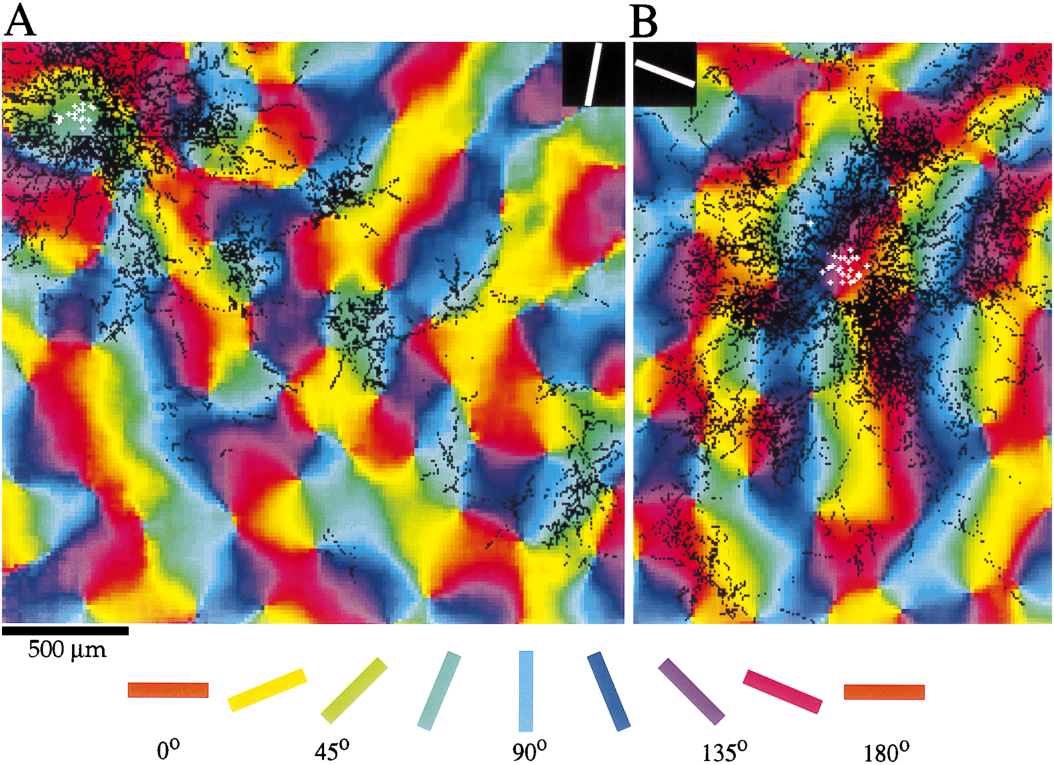
\includegraphics[width=0.6\textwidth]{BoskingLaterals.pdf}
	\caption[Patchy lateral connections overlaid on an orientation
      map. Reproduced from \cite{Bosking1997}.]{Illustrative
      examples of patchy lateral connections in the treeshrew visual
      cortex overlaid on an orientation map, clearly showing linking
      between iso-orientation domains. Reproduced from
      \cite{Bosking1997}.}
	\label{BoskingLatExc}
\end{figure}

The spatial scale of these connections has led several studies to
conclude that they may mediate modulation of RF-center properties in
the near surround \citep{Angelucci2002}. Lateral connections could
therefore provide a simultaneous mechanism for a number of observed
effects, including the expansion of the summation RF at low stimulus
contrast \citep{Sceniak1999}, co-linear facilitation
\citep{Mizobe2001}, and suppression from the near surround
outside the hsRF but within the lsRF
\citep{Sceniak2001,Levitt2002}. The previous section showed that such
phenomena could not be adequately accounted for by geniculocortical
afferents; measurement of spatial extents and response latencies of
horizontal connections reaffirm this view and have shown that the lsRF
and lateral connections are coextensive \citep{Angelucci2002}.

Apart from the exact spatial dimensions of horizontal connections, it
is important to highlight several other functionally important
properties. While layer 2/3 neurons display patchy connectivity,
linking regions with similar functional properties such as orientation
preference, this has been shown not to be the case in macaque layer 4B
and upper 4C$\alpha$ \citep{Angelucci2002}. In addition, it was found
that horizontal connections in macaque V1 are isotropic in visual
space, unlike the anisotropy along the axis of preferred orientation
observed in tree shrews \citep{Bosking1997} and several other
species. This could also indicate that orientation-specific contour
completion in macaques is mediated by feedback connections. Long-range
horizontal connections have been shown to elicit only subthreshold
responses \citep{Hirsch1991} and are thus limited to a modulatory
influence. However, as surround modulation extends far beyond the
monosynaptic spread of lateral connections, it is unlikely they
account for modulation from the far surround. Polysynaptic chains of
lateral connections are also an unlikely substrate for the far
surround due to the slow conduction velocity of their axons, and their
modulatory rather than driving nature. \cite{Bair2003} also showed
that onset latencies of suppression from the far surround were almost
equal to the delays from the near surround. This makes it likely that
far-surround modulation is mediated primarily by inter-areal feedback
connections, which we will look at in detail at a later stage.

Having established that spatial profile of lateral connections is
commensurate to that of the lsRF and vice versa, the data from both
sources will be laid out and analyzed. Anatomical data suggests that
the spatial spread of lateral connections can be anywhere between 3-10
mm (on average 6-7 mm) in total diameter \citep{Angelucci2002}. Along
its principal axis, the visuotopic monosynaptic spread of V1
horizontal connections has a mean of $2.47\degree \pm
0.3\degree$. This falls well within the range of estimates for the
lsRF as published in a number of studies
\citep{Shushruth2009,Sceniak1999,Sceniak2001}, which were fit with the
same integrated DoG model and stimulus protocol as used in the
\cite{Sceniak2006} paper on the spatial properties of LGN neurons,
reviewed previously.

In summary, there seems to be some agreement that lateral connections
could underlie the extent of the lsRF and mediate a number of effects
in the near surround, including contrast-dependent size tuning,
co-linear facilitation and iso-orientation contrast suppression.  The
extents of horizontal connections range between 3-10 mm, which
averages to around 2.5$\degree$ in visual space.

\paragraph{Feedback from Higher Cortical Areas and the Far Surround}

As the previous two sections have shown, modulatory influences to V1
RFs extend well beyond the spatial spread of both geniculocortical
afferents and horizontal connections. This extended modulatory field
is known as the far surround and is thought to be mediated by feedback
from higher cortical areas. The far surround has generally been
characterized as suppressive, especially for iso-oriented gratings in
the center and far surround. More detailed analysis has shown that the
far surround can also exhibit response facilitation under some
stimulus conditions. This section will characterize the function,
termination patterns and spatial extents of feedback connections from
higher cortical areas to V1.

The notion of a hierarchical organization of cortical visual areas has
been around for quite some time and more recent analysis of
feedforward and feedback connections has affirmed this view. At the
bottom of this hierarchy is V1, sending partially segregated FF
projections to areas V2, V3, V4 and the middle temporal (MT) visual area,
which all send FB projections back to V1
\citep{Felleman1991}. Feedforward projections from V1 to V2 arise
mainly from layer 4B and to a lesser degree from layer 2/3 and
6. Feedback connections, on the other hand, arise from layers 2/3A and
5/6 and terminate in the same layers from which FF connections are
sent, which means the cells projecting up the hierarchy often overlap
with the termination regions of FB projections being sent back down
\citep{Angelucci2002}.

Just like lateral connections, FB connections do not drive their target
cells, exhibiting only modulatory influence on the RF center
\citep{Bullier2001a}. Inactivation of areas V2 and MT has been shown
to reduce the firing rate of V1 neurons to stimuli in their RF center
\citep{Hupe1998}, suggesting FB inputs are summed with FF inputs to
increase activity. The exact balance between excitation and inhibition
of FB connections is so far not very well explored in macaques but
evidence from rats suggest that they almost exclusively target
excitatory cells. However \cite{Angelucci2006} and \cite{Schwabe2006}
have proposed a configuration where FB connections in the far surround
target pyramidal neurons, which in turn send monosynaptic horizontal
connections to excitatory and inhibitory neurons in the RF center and
can thus mediate both suppressive and facilitatory effects depending
on stimulus properties.

Feedback connections have been thought to underlie a number of top-down
effects in V1, including attention \citep{Treue2003} and the reverse
hierarchy theory of visual learning \citep{Ahissar2004}, but more
recent studies have suggested they contribute directly to the response
of V1 neurons to simple visual patterns
\citep{Angelucci2002,Angelucci2003,Schwabe2006}. Notably
\cite{Schwabe2006} and \cite{Ichida2007} seem to have resolved the
conflicting evidence about the far surround's dual suppressive and
facilitatory role. Using both experimental and theoretical work they
found that while the far surround is suppressive under high contrast
conditions, the response of a neuron to a low contrast stimulus in the
RF center is facilitated by a small annular stimulus in the far
surround. This indicates that excitatory and inhibitory surround
mechanisms have similar extents and that the sign of their
contribution depends on changes in local excitation/inhibition balance
brought about by surround stimulation.

Feedback projections from higher cortical areas to V1 mediate a number
of important contextual effects and have been implicated in the early
stages of visual attention, but also seem to be closely involved in the
processing of simple visual stimuli. This section has summarized
current knowledge on the spatial termination patterns of FB
connections to V1, indicating how they could give rise to functional
properties of V1 information processing. While the role of feedback
connections always needs to be taken into consideration, it will not be the
focus of this thesis, which will limit itself to afferent and lateral
connectivity in the primary visual cortex.  This limitation is
primarily for practical reasons, in that until suitable models of
extrastriate cortex are available, providing suitable feedback to V1
will remain very difficult and poorly constrained.

\section{The Internal Circuitry of Striate Cortex}

The previous section outlined the overall structure of the early visual
system, breaking down the contribution of inputs from various sources
on the receptive field (RF) of neurons in primary visual cortex
(V1). While this review provides general anatomical constraints and sheds
some light on the functional circuitry underlying many of the
contextual effects that have been observed in the primary visual
cortex, it does not address many of the fundamental questions about
the functional significance of recurrent cortical processing. In
particular, it does not address the delicate balance in both strength
and spatial extent between excitation and inhibition that is required
to halt runaway excitation, sparsify the inputs, and thereby allow for
the formation of concentrated activity bubbles around which
self-organization can take place. This section will cover how the
understanding of intra-cortical connectivity has evolved and how this
connectivity has been implemented in various developmental and
non-developmental models.

\subsection{The Mexican Hat} \label{MexicanHat}

Before complex tracing and circuit reconstruction techniques became
available, considerations about the connectivity profiles in the
cortex were largely theoretical or based on data from peripheral
regions, which were at the time more amenable to study. Anatomical
data and electrophysiological studies in the retina had shown that
there is a strong lateral inhibitory component involved in
decorrelating photoreceptor activities, thereby enabling more
efficient coding of the input \citep{Atick1992}. Lateral inhibition
was taken to be a general principle of sensory systems and, among
others, \cite{Blakemore1970} suggested repulsive interactions between
neighboring contours could account for psychophysical data. Further
evidence of lateral inhibition as a general feature of sensory systems
was provided by a variety of theoretical models of self-organization,
highlighting the necessity of effective local excitatory and 
long-range inhibitory interactions for the formation of local activity
bubbles, which in turn provided the basis for orderly map organization
\citep{VonderMalsburg1973,Miller1989}.

The connectivity profile employed in the various self-organizing map
models became known as the Mexican hat profile due to its strong
resemblance to a sombrero. A simulated Mexican hat profile is shown in
Figure~\ref{MexHat}, generated through a simple difference of Gaussian
(DoG) whereby a small excitatory Gaussian kernel is combined with a
larger inhibitory kernel. Numerous cortical models have successfully
employed this connection profile to explain a variety of effects
ranging from topographic map organization and orientation tuning to
contextual modulation. Problematically, it is unclear how biologically
realistic the assumption of strong local excitation and broadly tuned
and longer range inhibition really is.

\begin{figure}
	\centering \includegraphics[width=0.7\textwidth]{mexhat.pdf}
	\caption{A 3D plot of stereotypical Mexican Hat connectivity.}
	\label{MexHat}
\end{figure}

The fundamental question then is whether there exists a set of
connections that could account for the local excitatory and
longer-range inhibitory component. A theoretical model by
\cite{Kang2003} suggests that a relatively small isotropic but fast
inhibitory projection could account for the inhibitory component of
the Mexican hat. To get a better understanding of how the Mexican hat
might arise from a circuit where the excitatory connections are
actually generally much longer, we will therefore investigate the specific
circuits involved.

\subsection{Contrast dependence of suppression}

An interesting but related phenomenon is that suppression and
facilitation can arise in the same neuron under under different
stimulus conditions. Specifically the contrast levels seems to have
complex effects on the overall sign of modulatory inputs to a neuron.

Electrophysiological and optical imaging have both confirmed that
strongly driven cortical neurons receive strong net local excitation and
long-range lateral inhibition \citep{Grinvald1994,Sceniak2001}. At
high contrasts \cite{Grinvald1994} showed that a neuron responding to
a small, central grating stimulus in isolation exhibits far greater
levels of activity than when presented with a co-linear surround
stimulus alongside the central stimulus. This highlights an
interaction between the center and surround RF that is not only
dependent on the orientation statistics but also on the contrast
levels in the input. In particular \cite{Hirsch1991} and
\cite{Weliky1995} showed that lateral connections impinging onto a
neuron would exert a small excitatory effect, when embedded in a low
contrast surround, while high contrast would flip the sign of these
contextual influences and suppress the central neuron's
activity. Additionally, \cite{Hirsch1991} found that laterally evoked
EPSPs, presumably underlying facilitatory effects, experienced strong
voltage-dependent enhancement, speculating that this effect would allow
stimuli in the surround to modulate cRF responses without driving the
response on its own.

Precisely how these two input-dependent modes of contextual
integration emerge is unclear. However, as anatomical tracing
techniques have become more sophisticated and biomarkers for different
cell types were discovered, attempts have been made at identifying the
different cell and connection types involved in this circuit. These
anatomical surveys showed that long-range connections extending beyond
a single orientation column were almost exclusively excitatory, and
80\% of these excitatory synapses target other excitatory pyramidal
neurons \citep{Hirsch1991,Kisvarday1997a}. The remainder of these
connections were shown to target inhibitory interneurons, which would
in turn contact pyramidal neurons, suggesting a di- or poly-synaptic
mechanism for long range suppression. On the basis of some of this
work \cite{Douglas1991} developed what has become known as the
canonical microcircuit for the neocortex. This circuit includes
separate inhibitory and excitatory neurons, which are driven by
thalamic afferents and recurrent connections. Further work has fleshed
out the spatial profiles of these connections, which ultimately gave
rise to the simplified circuit described in
Figure~\ref{V1MicroCircuit}. This proposal goes some way toward
reconciling anatomy with the experimentally measured functional
connectivity profile at high contrast levels.

\begin{figure}
	\centering
        \includegraphics[width=0.25\textwidth]{weliky_microcircuit.pdf}
	\caption{Diagram presenting a proposed local microcircuit for
      long-range suppression through di- or poly-synaptic circuit in
      V1. Reproduced from \cite{Miikkulainen2005} as adapted from
      \cite{Weliky1995}.}
	\label{V1MicroCircuit}
\end{figure}

More recent attempts at reconciling anatomy with function have been
able to further resolve some aspects of the problem. In particular, there is
clear evidence showing that excitatory synapses onto excitatory and
inhibitory neurons differentially target their recipient
neurons. Excitatory connections onto inhibitory interneurons seem to
preferentially synapse perisomatically, in contrast with recurrent
long-range excitatory connections which have been shown to target
their recipient neurons dendritically
\citep{Gilbert1990,McGuire1991}. Additionally, at least a subset of
inhibitory interneurons seem to preferentially target the soma of
pyramidal and stellate cells they inhibit \citep{Markram2004}. On that
basis it is reasonable to assume that inhibitory connections are, in
general, stronger and may act divisively.

Although these divergent properties of excitatory and inhibitory
neurons were only discovered relatively recently, it had long been proposed that
inhibitory interneurons are inherently more effective at suppressing
activity than recurrent excitatory connections are at exciting the
network, but due to a high threshold or some other related mechanism
the inhibitory neurons are not strongly recruited unless there is
strong afferent input \citep{Sillito1979}, as would be the case under
high contrast conditions. Although it is now clear that network
effects allow for strong long-range inhibition through di- or
poly-synaptic connections under the right stimulus conditions, the
mechanisms by which contrast-dependent behaviors emerge from the
cortical circuit are still only vaguely characterized.

A number of models have been developed to explain contrast dependence
of contextual effects on the basis of the general principle of
asymmetry between the response properties of excitatory and inhibitory
neurons. One of the first to publish such a model were
\cite{Stemmler1995}, who suggested inhibitory neurons require higher
external input rates before activating because they receive
significantly less spontaneous background input as compared to
excitatory neurons, an effect known as stochastic resonance. Although
this mechanism has at least been theoretically reaffirmed
\citep{Bezrukov1997}, there is no experimental data establishing it as
a functionally significant mechanism in V1. Other models hoping to
account for a wider array of RF effects implement such a mechanism
directly by setting a higher threshold in the inhibitory population
and introducing very strong lateral excitation of inhibitory neurons
\citep{Schwabe2006}. Another suggestion was made by \cite{Somers1998},
who in addition to a simple threshold asymmetry, also point to the
claim by \cite{Thomson1994} and others \citep{Abbott1997,Tsodyks1997},
that synaptic depression causes recurrent excitation to quickly
decline in efficacy during high frequency stimulation, while
facilitation of excitatory synapses onto inhibitory interneurons
increases transmission efficacy as presynaptic firing rates increase
\citep{Thomson1995}.

The suggestion that inhibitory neurons have a higher contrast
threshold has become very popular in the theoretical literature of the
past 20 years. However, as of yet there is only limited evidence to
support this core assumption, and there are a number of alternative or
concurrent mechanisms that may explain all or at least some of the
contrast-dependent effects.

The fact that the V1 circuit seems to exhibit both a Mexican hat
profile and long-range facilitation, at least under some stimulus
conditions, seems contradictory. In particular, dissociating the
variety of different types of inhibitory interactions has been very
difficult from electrophysiological measurements alone. In order to
begin separating the origins of these different influences on a V1
neuron's response, we will therefore more closely investigate the
source of surround suppression in the cortex.

\subsection{Surround Suppression: Feedforward or Feedback?}

The last section highlighted how little we still know about the origin
of surround suppression and inhibition. There is still significant
controversy about whether surround suppression originates in feedforward or
feedback pathways or whether both contribute over different spatial
scales. The literature includes suggestions that suppression of the
classical RF by stimuli in the surround is mediated through synaptic depression in the
thalamo-cortical afferents \citep{Carandini2002}, broadly tuned
inhibition by thalamo-cortical recipients, long-range excitation of
local inhibitory interneurons, or even through various feedback
mechanisms. This section will detail the evidence for each of these
proposals and the possible anatomical origin of each of these mechanisms,
teasing apart the circuit by looking at interactions between
surround suppression, stimulus size, and contrast.

Since the circuitry of the cortex is so complex, the task of
identifying feedforward and feedback contributions to surround
suppression is difficult. Although only a starting point, one way of
roughly separating these two possible contributions is to look at
the time course of suppression. In the literature, early and late
contributors to surround suppression have been identified
\citep{Webb2005}. The early component is characterized as being driven
by lower CRF contrasts with spatio-temporally broadband tuning and
little adaptation \citep{Levitt1997,Cavanaugh2002a}. The late
component, on the other hand, is driven more strongly by high-contrast
stimuli in the CRF, has sharp spatio-temporal tuning, and can be
strongly affected by adaptation \citep{Levitt1997}. Evidence suggests
that the early, broadly tuned component originates in the LGN and the
thalamocortical recipient layer of visual cortex
\citep{Blasdel1984a,Hawken1996}. In monkey cortex in particular, this
broadly tuned suppressive effect is only weakly evident in the LGN and
is thought to arise much more strongly in layer 4 of striate cortex
\citep{Webb2005}, which may have some correspondence to the broadly
tuned inhibitory population identified by \cite{Hirsch2003}.

\cite{Carandini2002} on the other hand suggest that there is a
synaptic explanation for surround suppression, primarily due to the
speed with which the suppression arrives, its immunity to cortical
adaptation, and the fact that it is restricted to the CRF. However,
they concede that synaptic depression does not account for gain
control and the abolishment of cross-orientation suppression by
GABA$^{A}$ blockade, so a mechanism that can account for all these
phenomena may still be preferable. In that vein, \cite{Webb2005}
propose two inhibitory mechanisms, one of which sums local activity in
a neuron's CRF and divides the response of the CRF, and a later
component that receives inputs from a much larger area but provides
narrowly tuned suppression. The broadly tuned component in particular
has a strong relationship with contrast gain control, which has been
firmly established to act divisively. Independent work by
\cite{Xing2005} supports the suggestion of two inhibitory components
and further expands on the size dependence of these two
components. Specifically, \cite{Xing2005} conclude that the tuned component is
recruited far more strongly for larger stimuli, which seems to confirm
a contribution from beyond the CRF.

This recent work has identified two clear and distinct inhibitory
components, but has not yet fully described which mechanisms and
circuits by which they are mediated.  The next section will attempt to
address this shortcoming.

\subsection{Distinct Inhibitory Populations} \label{InhibitoryBackground}

In order to begin to understand the origin of intracortical surround
suppression mediated by various local inhibitory circuits, it is
necessary to consider the different candidate cell classes. While
there is a long list of different inhibitory cell types based on their
morphology and spiking behavior, recent techniques have divided
inhibitory cells into several broad, functionally distinct classes
based on their immunoreactivity. The two cell types considered here
are parvalbumin (Pv-ir) and somatostatin (Sst-ir) immunoreactive
neurons, which are primarily differentiated by the cellular locus of
their synaptic targets. While Pv-ir neurons seem to target pyramidal
cells perisomatically, Sst-ir neurons target their recipients
dendritically. Along with the Vasointestinal protein (VIP) expressing
interneurons these cell classes make up the majority of inhibitory
cells in the cortex. The following subsections will detail the
anatomical, physiological and functional differences between these
cell classes.

\subsubsection*{Parvalbumin Immunoreactive cells}

The two main cell types that are immunoreactive to parvalbumin are the
chandelier and basket cells \citep{Binzegger2004}. While chandelier
cells make up only a small fraction of GABAergic neurons in the cortex
and are primarily found in layer 2/3, the fast-spiking (FS) basket
cells are the predominant interneuron subtype in the mammalian cortex
across all laminae, accounting for 42\% in layer 2/3 and layer 5 and
78\% in layer 4 of the cat \citep{Hogan1992,Huxlin2001} and up to 74\%
across cortical layers in macaque \citep{VanBrederode1990}. The
abundance in the thalamocortical-recipient layers and the fact that
they preferentially target the soma and proximal dendrites of spiny
neurons with multiple strong synapses, exhibiting high probability of
GABA release \citep{Freund2007,Markram2004}, ensures that basket cells
are of tremendous interest. On that basis it has been suggested that
the perisomatic connectivity profile of basket cells gives them the
ability to provide shunting inhibition to layer 4 spiny neurons,
acting divisively to control their response gain \citep{Wilson2012}.

Basket cells can be further subdivided, primarily based on their size,
into clutch and large basket cells. However, all basket cells can make
multiple connections onto a target pyramidal neuron
\citep{Somogyi1983} and have a considerable spatial extent
\citep{Kisvarday2002}. In particular, studies in cat area 17 and
macaque V1 have identified basket cells 1-2 mm in extent
\citep{Somogyi1983,Lund1987,Lund1991,Martin1983} and single-cell
tracing studies have even identified large basket cells, which give
off a roughly uniform number of boutons across a large diameter
extending up to two hypercolumns \citep{Buzas2001}, which corresponds
to about 1.5 mm in macaque. A schematic representation of the basket
cell connectivity profile is summarized and compared against both the
orientation column structure and the excitatory connection profile in
Figure~\ref{BasketCellExtent}. Functionally such a connectivity
profile may indicate that basket cells can suppress neurons with
widely varying orientations, which may implicate basket cells as an
important mechanism to sharpen orientation preference and would also
lead to cross-orientation contextual effects.

\begin{figure}
	\centering
        \includegraphics[width=1.0\textwidth]{basketcellextent.pdf}
	\caption[Schematic representing the proposed spatial distribution
      of pyramidal and basket cell extents and their relationship to
      the orientation map in V1. Reproduced from
      \cite{Buzas2001}.]{Summary schematic comparing relationship
      between long-range basket cell and excitatory connectivity with
      the underlying orientation preference structure. Upper legend
      represents different orientation domains in the cortical
      topographic map. Grey dotted lines indicate the orientation
      column within which the soma of the simplified basket cell and
      excitatory neuron are found. The grey field with minus signs
      indicates the extent of inhibition provided by the basket cell
      connections considered in the current study. The grey region
      with plus signs indicates the excitatory field of a
      stereotypical pyramidal cell, based on previous data by
      \cite{Bosking1997,Kisvarday1997a} and others. The height of the
      grey plus/minus regions indicates the number of axon terminals
      provided in that column. While basket cell terminals show local
      maxima every half hypercolumn distance, pyramidal cell terminals
      are maximal at every full hypercolumn distance. Reproduced from
      \cite{Buzas2001}.}
	\label{BasketCellExtent}
\end{figure}

In terms of their spiking behavior Pv-ir cells are typically
characterized as being fast fast-spiking (FS) neurons, often firing in
bursts with a very short response latency. It is important to note
however that not all fast-spiking cells are immunoreactive for
parvalbumin and that not all PV neurons are fast-spiking. Further,
evidence from somatosensory cortex in rodent and lagomorph species
suggests they receive strong input from thalamocortical afferents
arriving in layer 4 and very effectively suppress sustained firing
from spiny neurons receiving inputs from the thalamus
\citep{Swadlow2003}, implicating them in feedforward inhibition. A
possible feedforward inhibition circuit is shown in
Figure~\ref{burkhalterpv}. Their effectiveness in suppressing
feedforward activity can be explained by the large number of
thalamocortical axons they receive, which exhibit faster kinetics than
those targeting spiny neurons \citep{Cruikshank2007,Gabernet2005}, and
the fact that they evoke large inhibitory responses in spiny cells
\citep{Cruikshank2007,Gabernet2005}.

It is also important to note that the thalamocortical synapses onto
the Pv-ir population have been shown to be depressed by repetitive
activation, resulting in weaker feedforward inhibition at high
stimulation frequencies \citep{Gabernet2005}, a property which may
indicate lower activation of the PV population at high contrasts. The
Pv-ir population may also play an important role in network
homeostasis, as activity blockade has been shown to decrease the
efficacy of Pv-ir inhibition \citep{Bartley2008}, thereby indirectly
up-regulating activity in excitatory cells. Further, selectively
up-regulating Pv-ir cells using optogenetic stimulation was shown to
have a similar effect as lowering the contrast, which is to increase
preferred size and weakening surround suppression
\citep{Nienborg2013}. This evidence is compatible with the idea that Pv-ir
neurons provide strong feedforward inhibition such that the input
drive in the cortex is decreased, as would be observed under 
low-contrast conditions. Overall then, Pv-ir neurons show strong
interaction with stimulus contrast and may be involved in regulating
the gain of the network, with complex implications for the contrast
response of the network.

\begin{figure}
	\centering
        \includegraphics[width=1.0\textwidth]{burkhalter_pv.pdf}
	\caption[Proposed inhibitory circuit for feedforward inhibition
      mediated by PV cells. Reproduced from
      \cite{Burkhalter2008}.]{Inhibitory networks involving
      fast-spiking parvalbumin-immunoreactive neurons in
      thalamocortical, interlaminar, and interareal cortical
      circuits. Feedforward excitatory thalamocortical inputs to
      pyramidal cells, spiny stellate neurons ($\blacktriangle$) and
      fast spiking interneurons ($\newmoon$) in layers 2-4 (a). Inputs
      to interneurons are stronger (large arrowheads) than inputs to
      spiny cells. PV neurons provide strong (large rectangular
      endings) feedforward inhibition (b) to spiny cells. Feedback
      inhibition (c) results from PV neurons that are excited by the
      same spiny neurons that they inhibit. These reciprocally
      connected spiny neuron/PV neuron pairs share common inputs
      (e.g., cells in layer 4 from thalamus or cells in layer 2/3 from
      layer 4) creating recurrent excitatory (d) and inhibitory
      subnetworks (contained within blue shaded boxes). ‘Lateral’
      inhibition (e) of these subnetworks results from PV neurons that
      are driven by excitatory feedback connections (f) from outside
      the subnetworks (e.g., by layer 5 to layer 2/3 connections or
      feedback from higher cortical areas). Notice that ‘lateral’
      inhibition is weaker (small rectangular endings) than
      feedforward and feedback inhibition and impinges on multiple
      subnetworks. Reproduced from \cite{Burkhalter2008}.}
	\label{burkhalterpv}
\end{figure}

There is still considerable debate on the extent to which this
subpopulation is tuned to a particular orientation. Most
visuo-cortical models employ broad, non-specific GABAergic inhibition
\citep{Somers1998,Troyer1998}. This seems to be supported by
anatomical evidence, which has long shown that inhibitory projections
are generally diffuse and display low specificity for specific
stimulus features \citep{Albus1994,Kisvarday1997a}. Further,
electrophysiological data paints a similar picture, revealing
suppression that is broadly tuned for stimulus attributes, providing
orientation-unspecific suppression from a visual region that is
coextensive with the classical RF \citep{DeAngelis1992}. Recent
attempts at studying the Pv-ir neurons at the single-neuron level have
revealed a mixed picture. While the cells as a whole were broadly
tuned to various stimulus features, individual branches often
displayed very high specificity, which may underlie subfield
antagonism and contribute to a push-pull configuration
\citep{Kisvarday2002}. 

Studies in mouse visual cortex seem to confirm such a dual purpose of
Pv-ir neurons, although they also find higher heterogeneity in the
Pv-ir population \citep{Runyan2010}. This result may indicate a
laminar differentiation in function, as studies of Pv-ir neurons in
the thalamocortical recipient layer 4 have characterized them to
exhibit very broad tuning, due to their low spiking threshold and more
convergent inputs \citep{Ma2011}. However, even in layer 2/3 most
mouse Pv-ir cells displayed broad orientation tuning
\citep{Hofer2011}. Further studies in cat area 17 find very similar
results identifying a class of inhibitory complex cells in layer 4
exhibiting weak orientation tuning \citep{Hirsch2003}, which can
primarily be accounted for by the tuning of synaptic responses and a
lower spike threshold \citep{Nowak2008}.  A more recent study in
auditory cortex seems to affirm these conclusions, hypothesizing that
`while PV neurons may provide broadly tuned feedforward inhibition for
a rapid control of ascending inputs to excitatory neurons, the delayed
and more selective inhibition from SOM neurons may provide a specific
modulation of feedback inputs on their distal dendrites`
\citep{Li2014}. However, a more extensive study in layer 4 of the cat
found no significant broadening in the synaptic orientation tuning of
fast-spiking interneurons over that exhibited by regular spiking cells
in the same region \citep{Cardin2007}; only when looking at spiking
responses was a significant broadening found. As an explanation of
this apparent difference in tuning between rodents, which exhibit no
orientation maps, and primates or carnivorans, it has been suggested
that these cells pool the input from nearby neurons and inherit their
orientation preference \citep{Isaacson2011}. There may also be a
layer-specific segregation in their function providing push-pull
suppression in thalamocortical recipient layers and broader inhibition
in upper layers.

Based on our current knowledge of Pv-ir cell population and more
specifically the basket cells, it is clear that they provide a good
candidate mechanism to account for a number of important
phenomena. Their fast response profile, large spatial extent and
seemingly broader orientation tuning may allow them to carry out fast,
adaptive gain control and broadly tuned suppression, thereby
sharpening the orientation preference of the PNs in their vicinity.

\subsubsection*{Somatostatin Immunoreactive cells}

The Sst-ir population has been characterized to a lesser extent, but a
general consensus is beginning to emerge around their function and
electrophysiological properties. The Sst-ir cells account for around
half of the non-PV-expressing neurons \citep{Gonchar2007,Xu2010} and
preferentially synapse onto distal dendrites and dendritic tufts of
pyramidal neurons \citep{DiCristo2004,Silberberg2007}, on the basis of
which it has been suggested that Sst-ir neurons act subtractively
\citep{Wilson2012}.

In trying to characterize the excitatory inputs to Sst-ir cells in
layer 2/3 of the mouse, \cite{Xu2009} determined that unlike Pv-irs,
the main source of excitation of Sst-irs were horizontal axons within
layer 2/3, not the ascending layer 4 axons. This property also
contributed to the size-dependent responses of the Sst-irs, which were
shown to be recruited progressively more strongly when they were
exposed to optogenetic photostimulation of increasing
diameter. Importantly, the Sst-ir response grew larger even when
photostimulation reached beyond its maximal dendritic extent,
demonstrating that the recruitment of increasingly more distant
pyramidal cells provided their main excitatory drive. This putative
circuit is shown in Figure \ref{som}, exhibiting their pooling of
tuned, excitatory input from pyramidal cells across a large area
yet providing only very local inhibition. It also seems that
Sst-ir interneurons are capable of disinhibiting the thalamocortical
recipient layer 4 by targeting Pv-ir cells \citep{Xu2013}.

In terms of their response properties, mouse visual cortex Sst-ir
neurons have been shown to exhibit much lower levels of spontaneous
and evoked activity, stronger orientation and direction selectivity,
and longer response latencies than Pv-ir neurons \citep{Ma2011}. These
properties are consistent across both layer 2/3 and 4 and may point to
a role in gating later-arriving intracortical excitatory inputs. In
terms of their tuning properties, Sst-ir neurons display smaller
On/Off subfields with less overlap than nearby spiny neurons and
orientation tuning, on par with pyramidal neurons. While most data on
their tuning properties comes from rodent visual cortex, which does
not exhibit a topographic organization of orientation tuning, it seems
the stronger orientation selectivity of Sst-ir cells can be accounted
for by their preferential connectivity to neurons with similar
orientation preference as well as a higher spiking threshold and
weaker excitatory inputs \citep{Bartley2008}. Another interesting
feature of Sst-ir response properties is the fact that although their
excitatory inputs are weak, those inputs are facilitatory, resulting
in delayed but strong activation under high frequency stimulation
\citep{Beierlein2003,Bartley2008,Tan2008}. Based on these properties,
Sst-ir neurons would only be recruited to provide significant
inhibition if the stimulus contrast or size reaches a certain level
\citep{Adesnik2012}. Thus they could provide a direct mechanism for
contrast-dependent size tuning and surround-modulation effects, being
only weakly recruited when contrast or stimulus size is low but
becoming strongly activated at higher contrast levels and for larger
stimulus sizes, providing a possible circuit mechanism for
\cite{Sillito1979} proposal for surround suppression.

Another suggested role for Sst-ir neurons is the gating of feedback
signals on the distal dendrites of principal neurons. Martinotti
cells, which provide strong axonal projections to layer 1 of the
cortex, make up a large proportion of Sst-ir neurons in layer 2/3 of
the cortex and are therefore well placed to suppress feedback signals
arriving in the superficial layers of the cortex
\citep{Fanselow2008,Gentet2012}. In the rodent somatosensory cortex,
\cite{Gentet2012} showed that Sst-irs in layer 2/3 become
spontaneously active during passive wakefulness but are strongly
suppressed during active whisking behavior, presumably by the
vasoactive intestinal peptide (Vip)-ir population discussed below. The
Sst-ir cells may therefore be involved in mediating top-down control
of sensory processing, effectively gating context-dependent processing
in a state-dependent manner.

\begin{figure}
	\centering
        \includegraphics[width=1.0\textwidth]{adesnik_som.pdf}
	\caption[Schematic proposing Sst neurons' role in integrating
      long-range inputs. Reproduced from
      \cite{Adesnik2012}.]{Schematic illustration of the cortical
      circuit in layer 2/3 contributing to surround suppression. As a
      visual stimulus expands (larger stimuli are shown in lighter
      grey), recruitment of adjacent principal cells (PCs) increases
      Sst-ir excitation through horizontal axons (horizontal
      arrows). Reproduced from \cite{Adesnik2012}.}
	\label{som}
\end{figure}

In summary, Sst-ir neurons seem to provide delayed and
feature-selective feedback inhibition, which puts them in a good
position to effectively gate late-arriving intracortical excitatory
inputs originating in either lateral or feedback connections, but may
also be implicated in suppressing feedforward inhibition by
inactivating layer 4 Pv-ir cells.

\subsubsection*{Vasointestinal peptide expressing interneurons}

The material reviewed so far has focused primarily on the two most
common types of inhibitory interneurons, the Parvalbumin (PV) and
Somatostatin-expressing (Sst) cells.  Since that initial work, a
number of studies have focused on the role of 5HT3ar-expressing
interneurons and particularly the vasointestinal peptide
(Vip)-expressing subgroup \citep{Lee2013, Fu2014, Higley2014,
  Kepecs2014}.

The Vip subgroup is particularly concentrated in upper, associative
layers and feedback layers of the cortex, as shown in
Figure~\ref{GABADistribution} by \cite{Rudy2011}. The most striking
finding was their central role in state-dependent modulation during
active whisking tasks in rodents. \cite{Lee2013} found that
S1-projecting vM1 pyramidal neurons strongly recruited Vip-expressing
interneurons in superficial layers of somatosensory barrel cortex,
which in turn inhibited somatostatin-expressing interneurons causing
effective disinhibition of cortical pyramidal cells. These results
were then affirmed through optogenetic stimulation of Vip neurons in
mouse V1, artificially mimicking the effects of locomotion
\citep{Fu2014}. When considered in conjunction with previous studies
that established strong cholinergic and nicotinic inputs to Vip
neurons from the basal forebrain \citep{Wickersham2009}, the evidence
suggests a strong involvement of Vip neurons in a cortical circuit
responsible for the enhancement of activity in sensory cortex by
behavioral state.

\begin{figure}
	\centering
        \includegraphics[width=0.4\textwidth]{GABADistribution.pdf}
	\caption{Distribution of GABAergic interneurons in mouse S1 cortex
      by immunohistological marker. Reproduced from \cite{Rudy2011}.}
	\label{GABADistribution}
\end{figure}

\subsubsection*{Connectivity between different cell types}

In order to gain an understanding of the circuits the different
interneuron cell types are involved in, it is important to consider
their interconnectivity. Several studies have sought to determine the
connectivity between Pv-ir, Sst-ir and other interneuron types. The
core findings of these studies determined that Pv-ir cells
preferentially inhibit one another, Sst-expressing cells avoid one
another and inhibit all other types of interneurons, particularly the
Pv-ir cells \citep{Xu2013}, while a third type, the Vip-ir cells
preferentially inhibit Sst-ir cells \citep{Pfeffer2013}. This
connectivity profile is schematically represented in
Figure~\ref{gaba_circuit}. In mouse cortex the Pv-ir, Sst-ir and
Vip-ir cells accounted for about 40\%, 18\% and 8\% of the GABAergic
population, respectively \citep{Xu2010}, and although these
percentages vary considerably across species Pv-ir and Sst-ir are
always the two most commonly expressed GABAergic populations.

\begin{figure}
	\centering
        \includegraphics[width=0.7\textwidth]{pfeffer_gabacircuit.pdf}
	\caption{Connectivity between somatostatin (Sst),
        parvalbumin (Pv), vasoactive intestinal peptide (Vip)
        expressing and pyramidal (Pyr) cell types. Adapted from
        \cite{Pfeffer2013}.}
	\label{gaba_circuit}
\end{figure}

\section{GABAergic regulation of plasticity and column structure}

Experience-dependent plasticity has been shown to shape the
organization of the sensory cortex during an initial critical period and
beyond. Dark-rearing \citep{Fregnac1978} and monocular-deprivation
(MD) experiments \citep{Shatz1978} in particular have confirmed the
fundamental importance of sensory experience in shaping the
development of the cortex. The mechanisms controlling the onset of the
critical period and regulation of plasticity thereafter have also been
studied extensively.  A large body of evidence points to the
important role of the inhibitory neurotransmitter
$\gamma$-aminobutyric acid (GABA) in regulating synaptic
plasticity. However, as the above paragraphs have shown, the population
of GABAergic neurons is highly heterogeneous with hugely divergent
anatomical and functional profiles. Using specific pharmacological and
genetic populations, it has been possible to narrow down the
involvement of certain interneuron subtypes in shaping critical-period
plasticity and column structure in the cortex.

One of the first indications that GABAergic circuits are involved in
shaping plasticity came when it was shown that a gene-targeted
disruption of the GABA synthetic enzyme glutamic acid decarboxylase 65
(GAD65) could delay critical period onset indefinitely
\citep{Fagiolini2000}. In order to further narrow down the specific
GABA circuits underlying visual cortical plasticity, more specific
pharmacological manipulations were required. On that basis
\cite{Fagiolini2004} used benzodiazepine infusions, known to
selectively enhance GABA type A ($GABA_A$) receptor-mediated currents
through the $\alpha1$ subunit \citep{Rudolph1999}, in conjunction with
MD to prematurely trigger ocular dominance plasticity in mice. These
$GABA_A$ receptor-$\alpha1$ subunits are preferentially enriched at
somatic synapses receiving input from Pv-ir large basket cell
terminals \citep{Klausberger2002}, strongly implicating large basket
cells in visual cortical plasticity.

Beyond controlling the timing of critical period plasticity, further
experiments using benzodiazepines have shown strong effects on the
columnar organization of the cortex. The experiment by
\cite{Hensch2004} locally infused regions of cat area 17 with the
$GABA_A$ agonist diazepam and an inverse agonist (DMCM) and studied
the effects on ocular dominance columns. Chronic treatment with
diazepam had little effect in the functional properties of mature
cortical neurons in vivo apart from enhancing inhibitory postsynaptic
currents. However, the treated hemisphere exhibited reduced
binocularity of single unit responses and wider OD columns near the
infusion site. Infusion with the benzodiazepine inverse agonist DMCM
had the inverse effect, resulting in less discrete and narrower
columns near the infusion site. These results suggest that the
diazepam-mediated enhancement in competition reduces binocularity of
single-unit responses, as well as sharpening and widening the
anatomical segregation of monocular regions near the infusion
site. This once again suggests that $GABA_A$ inhibitory currents,
primarily originating from Pv-ir neurons in the cortex, are
fundamentally important to shaping the plasticity and organization of
the cortex.

In order to establish how ocular dominance plasticity emerges during
monocular deprivation, \cite{Kuhlman2013} developed even more
precisely targeted pharmacological manipulations. By selectively
expressing specific receptors on Pv-ir cells they were able to
selectively up- and down-regulate their activity. Their results
indicate that a rapid but transient reduction in Pv-ir cell firing
restores pyramidal cell firing to pre-deprivation levels, allowing
competitive plasticity to occur. Pv-ir neurons therefore seem to play
a permissive role in visual cortical plasticity. Interestingly, adult
sensory plasticity such as reinforced associative learning occurs
through a similar mechanism, where cholinergic activation of layer 1
interneurons suppresses Pv-ir neural activity allowing associative
fear learning to occur \citep{Letzkus2011}. All this work suggests a
crucial role for Pv-ir neurons in controlling cortical plasticity
during the critical period and beyond.

\section{Contextual Modulation and Attention} \label{contextualmodulation}

Arguably, the computational task in vision is to map visual experience
to the cortical representation of that particular stimulus or if no
such representation already exists, to extract lower level features in
order to encode them for future reference. Using this statistical
model the brain is then able to decide which visual features carry
behavioral importance and which can be safely ignored. As such the
neocortex has to combine prior information with the incoming
information stream and quickly and reliably identify the most salient
stimuli. It has often been argued that this process is mediated by
bottom-up and top-down processes, although it seems likely that there
is close coupling between the two. This section will outline
high-level models of attentional modulation, and attempts to
understand the neurobiological processes behind them and more basic
contextual modulation phenomena that may underlie many of these higher
level effects.

\subsection{Contextual and Attentional Phenomena in V1}

A number of phenomena associated with attention and contextual
modulation, including iso-orientation suppression or facilitation,
boundary detection, contour completion and noise exclusion have been
observed in V1. Although these phenomena are generally associated with
bottom-up attention, they lay the foundation for higher level phenomena
such as pop-out and figure-ground segregation and may reveal more
about general mechanisms applying also to higher visual areas.

Basic contextual effects such as iso-orientation suppression have
already been discussed and models have begun to suggest the functional
connectivity mediating implicating both lateral and feedback
connections. \cite{Li2002} has proposed that pre-attentive
bottom-up processes allow V1 to generate a saliency map of the visual
input. However, the fact that higher cortical areas have also been
associated with saliency signaling and the lack of long-range
intra-areal connectivity in V1 suggest that while it can encode local
saliency, feedback is required to globally integrate saliency across
visual space.

Feedback modulation of V1 activity has been implicated in a number of
effects, spatial attention being chief among them. Spatial attention
is thought to be able to select multiple low- and high-level objects in
the visual space across V1 and higher visual areas
\citep{McMains2004}. Spatial attention is thought to underlie noise
exclusion \citep{Dosher2000} and may be explained by effects similar
to what has been experimentally observed during iontophoretic application
of ACh. Other effects that have been commonly associated with
feedback in some form are the signaling of illusory contours, which
have been shown to be negatively signaled or deemphasized in V1
\citep{Ramsden2001} and boundary detection \citep{Poort2012}.

\section{Natural Image Statistics, Sparsity and Horizontal Connections}

It has long been hypothesized that connectivity in the cortex captures
the statistics of the sensory input in order to perform predictions
and maintain sparse representations of subsequent inputs \citep{Field1993,
  Simoncelli2001}. These effects cover both that the distribution of visual
features that are thought to sparsely represent the visual features of
world \citep{Olshausen1996}, but also suggests that it captures the
Gestalt law of good continuation in the form of so-called association
fields, which preferentially link neurons which represent edges on a
continuous contour \citep{Field1993}. Separately a wide range of work
has explored the distributions of light intensities, color statistics
and spatial correlations in natural images. In particular, the
power-law distribution of spatial frequencies in natural images has
been widely discussed in the literature, but ultimately this property
largely seems to reflect scale invariance within natural images
\citep{Ruderman1997}.

Numerous studies and models have since been devised to address whether
the visual system takes advantage of the correlational structure of
natural images. These types of normative models were able to show that
surround inhibition, whether subtractive or divisive, could cancel out
correlations, effectively whitening or decorrelating the activity in
the visual system \citep{Srinivasan1982, Atick1992}. In doing so they
quickly found that simple decorrelation was not sufficient to
optimally represent natural images, because whitening does not
eliminate all structure in a natural image; e.g., edges and lines
remain. By introducing an explicit sparsity constraint,
\cite{Olshausen1996} were able to develop V1-like simple cell
receptive fields with varying orientations, spatial frequencies and
sizes. These models suggested that the sensory system was optimizing
two constraints, sparsity and statistical independence. However, even
these approaches cannot achieve complete statistical independence,
since there are higher-order correlations even between non-overlapping
receptive fields.

By introducing divisive normalization, \cite{Schwartz2001a} were able
to show that these types of dependencies could be further
eliminated. Furthermore, the weights used in the computation of the
normalization signal could be specifically optimized to maximize the
independence of the normalized responses. Additionally, they
demonstrated that the optimal weights were at least partly due to the
prevalence of extended contours in natural images.

Attempting to quantify the co-occurence statistics of contours in
natural images, \cite{Geisler2001} demonstrated that the performance
in contour-detection tasks could be predicted by a local grouping rule
derived from the co-occurence statistics. The first explicit link to
horizontal connectivity was made by \cite{Sigman2001}, who noted that
the pattern of long-range patchy connectivity in the primary visual
cortex linking iso-orientation columns has a close correspondence with
the observation of co-circularity in natural image statistics. Noting
the processes of iso-orientation suppression and contour integration,
they argue that iso-orientation suppression may serve to further
reduce redundancies in neural coding, thereby achieving greater
statistical independence, which would explain why neural responses
appear most sparse when presented with natural stimuli. Furthermore
recent findings have shown that low-level co-occurrence are sufficient
to classify images of animals \citep{Perrinet2015}, suggesting that
even early visual areas could be involved in high-level classification
tasks. Secondly, observing that visual cortex can also exhibit
co-linear facilitation under low-contrast conditions
\citep{Sceniak1999, Kapadia1999}, they suggest that under low
signal-to-noise conditions the cortex may act to enhance commonly
encountered patterns to aid the identification of contours and form.

These theoretical studies have hugely advanced our thinking about the
computations performed by the early visual cortex, yet very little
work has been done to look at the actual structure of horizontal
connectivity in V1, largely due to the difficulty in obtaining data
from more than just a few cells. Even on the question of whether
horizontal connections are anisotropic along the axis of preferred
orientation of the neuron, as would be expected from theoretical
studies, there is conflicting evidence. The result has been confirmed
in monkey \citep{Sincich2001}, tree shrew \citep{Bosking1997} and cat
\citep{Schmidt1997}, but conflicting results have been reported for
macaque \citep{Angelucci2002}. By performing analyses on a tree-shrew
dataset from 1997, \cite{Hunt2011} investigated whether horizontal 
connections captured the co-circularity of natural image
statistics. Although they found neurons that exhibited co-circularity
and anti-cocircularity and hypothesize a role for both, given the
small number of lateral connections fields and the fact that
second-order properties are highly sensitive to even small errors in
the data, it is unclear how strong this result is. Further research in
this area is desperately needed if we are to understand how the
patterns of lateral connectivity relate to natural image statistics.

\section{Existing large-scale models of the primary visual cortex}

In the previous sections we laid out a wide range of evidence
relating specific empirical studies to each other, to begin teasing
apart how low-level interactions can give rise to complex behaviors. A
wide range of modeling work has been targeted to that very
question, and there exists a wide breadth of models attempting to model
the function of the visual cortex at the level of individually spiking
neurons or modeling looking specifically at the surround modulation
interactions between neurons. Here we will review some of these
models, highlighting why although many models explain specific
phenomena well, the lack of development and learning means that these
models are static and cannot easily explain the dynamic, adaptive
nature of computation in the cortex.

\subsubsection*{Large-scale spiking models} \label{LargeModels}

With the introduction of increasing computational power it has become
feasible to model large networks of spiking neurons, allowing
simplified models of the visual cortex to be created. In particular,
large scale simulators such as NEURON \citep{Hines1994}, NEST
\citep{Gewaltig2007} and interfaces such as PyNN \citep{Davison2009}
have made it possible to specify complex neural network models at the
level of individual neurons and even synapses and ion channels.

These models generally replicate the statistics and rough spatial
scales of different types of connections, between different cell
classes and investigate the response of the model at resting state or
when provided with thalamic input \citep{Shelley2002,
  Potjans2014}. Additionally there are also even larger models
attempting to model the visual cortex just as one area of a complex
brain network \citep{Eliasmith2012}. What these models have in common
is that they are not well suited towards addressing the kinds of
question most vision scientists are interested in, particularly in
regard to the way the visual cortex can extract and encode the
statistics of the visual input and give rise to well-studied effects
like contextual modulation. Instead these models are usually used to
study only the overall statistics of the responses. As an example,
\cite{Potjans2014} develop a highly detailed and refined microcircuit
model of the visual cortex, including different cell types and laminar
distributions, which they can scale to large cortical networks. The
resultant model can provide answers about the flow of information in
the network between different layers, but because it is simply a
statistical model of connectivity it cannot address questions at the
functional, algorithmic, or computational levels.

Alternatively, there are large-scale models that disregard the
architecture of different brain regions entirely, instead treating
them as modules of excitatory and inhibitory cells serving
a specific function. \cite{Eliasmith2012} present one such model,
which models the entire cortical hierarchy and even performs specific
tasks. Here the model of V1 is simplified to the point where it is
simply a visual encoder, ignoring more complex interactions entirely.

As we have seen, models of this scale suffer of one of two
problems. When incorporating a lot of biological detail, they are very
useful for understanding the low-level interactions in a network and
how information is communicated locally, but are not usually useful
for linking low-level processes to the higher-level processes that
these processes underlie. Models at the other extreme are relegated to
be very high-level approximations of the visual cortex, without the
full breadth of complex contextual effects that has been observed in
the visual cortex.

\subsubsection*{Surround modulation models} \label{SRmodels}

Perhaps the precisely opposite approach to building in copious amounts
of biophysical detail is to focus on a particular phenomenon and
attempt to explain it with a reduced set of mechanisms. These models
have traditionally been incredibly useful in explaining different
aspects of the literature in V1. Specifically, point, rate-based
neuron models have been used to explain effects ranging from surround
suppression and to more complex contextual-modulation effects such as
contour integration and pop-out.

The surround-modulation literature is one of the most complex topics
in visual neuroscience, due to the high dependence of the observed
phenomena not only on the precise stimulus conditions but also the
behavioral state of the animal. As we discovered in
Section~\ref{contextualmodulation}, there are two main phenomena that
are of interest: surround suppression, usually thought to reduce
redundancy in the input, and contextual enhancement of responses
through facilitatory effects. These two opposing mechanisms are
thought to drive a wide range of the phenomena in the literature
including pop-out, contour completion, as well as end stopping,
flanker facilitation, and much more.

Various models have been proposed to explain how these contextual
influences emerge. In one of the more straightforward models,
\cite{Li2002} proposes that through recurrent enhancement of
responses, long-range lateral connections can give rise to a visual
saliency map in V1, which underlies pop-out, enhancing features that
stand out from the visual background. While this model explains how a
particular surround modulation effect can emerge from the network
interactions between neurons with different tuning properties, it does
not account for both suppressive and facilitatory effects and since it
is highly abstract cannot shed light on the precise interactions that
could give rise to both in a circuit.

Other models such as the \cite{Schwabe2006} model break down the
interactions from different sources in more detail demonstrating how
long-range patchy horizontal connectivity can mediate both excitatory
and inhibitory influences from the surround. Unlike previous models
they suggest that long-range feedback connections could be the main
driver of these contextual influences and that the drive to inhibitory
neurons in the local circuit determines the sign of the
effect. However, since this is a static model it provides no account
of how the required lateral or feedback connectivity could emerge and
since the model only represents 1D space cannot process realistic
stimuli. Additionally this model still uses the assumption originally
made by \cite{Somers1998}, that inhibitory neurons have a higher
threshold than excitatory neurons, to account for contrast dependent
effects, which has received little experimental confirmation.

An alternative to this circuit-level analysis is to express these
interactions in the more abstract framework of predictive coding. The
work by \cite{Spratling2010} in particular expresses the cortical
circuit as predictive coding, modeling the response of V1 neurons
using a competitive mechanism between neurons attempting to best
represent the input. Like many others, this model provides a good
account of various surround modulation effects including iso- and
cross-orientation suppression but exhibits only weak facilitatory
effects, suggesting that it does not fully capture the mechanism that
is behind the contrast- and context-dependent interactions between
suppression and facilitation. Furthermore, it is very difficult to
relate the interactions between explicitly predictive or error-coding
neurons to the real interactions taking place in the cortex.

Then there are a class of phenomenological models attempting to
explain a variety of surround modulation effects based on the
geometries found in visual fields and the Gestalt law of good
continuation \citep{Field1993}. The \cite{Keemink2015} model, for
example, suggests that effects including the tilt illusion and contour
detection can be explained by a single mechanism, which computes the
elastica curvature energy of the smoothest contour connecting oriented
bars. This suggests that the visual cortex can somehow compute the
energy required to connect different contours but does not explain how
this association field could emerge. It is therefore a good account of
what the cortex is computing, but does not provide a canonical
mechanism for how these interactions can emerge independent of the
sensory modality that is involved. A general mechanism would allow the
model to extract the statistical dependencies between arbitrary
features, such that when trained on natural images it automatically
extracts the geometric relationships within contours.

Another avenue of study has been the approach by the Schwartz lab, who
have for a long time investigated the interaction between
natural-image statistics and surround-modulation effects. This is
perhaps one of the most interesting approaches, because it treats
contextual phenomena not as a by-product of some underlying
computational process, but rather supposes that they are driven by the
statistics of the visual input and are therefore closely tied to the
computational task that is actually being solved. In \cite{Coen2015}
they describe an extension of a simple normalization framework that
computes the homogeneity in an image between center and surround,
gating the divisive normalization component accordingly, which
directly leads to feature-specific surround modulation effects
observed in experiments. In this framework, surround modulation is
simply the measurable effect of statistical inference, improving the
efficient encoding of the stimulus.

All of these models capture important parts of the phenomena involved,
highlighting how network interactions between neurons with different
tuning properties can give rise to complex contextual modulation
effects \citep{Li2002}, where the sources of this input could
originate from \citep{Schwabe2006} and how these interactions might
fit into a general computational paradigm that is concerned with
prediction and inference \citep{Spratling2010, Coen2015}. However, all
of these models are static, presupposing an existing profile of
connectivity, and thus cannot directly address how different cell
types could interact to give rise to a circuit, mechanistically
explaining how these effects emerge.

\subsection{Developmental models} \label{devmodels}

As it is thought that the cortex captures statistics about the sensory
streams to construct internal models of the world, it is clear that
function, structure and development are closely linked. Indeed it is
now clear that V1 is a dynamic and adaptive circuit, which exhibits
learning and learns to optimally encode and represent its inputs. In
other words, V1 is not a static circuit, organizing solely based on
genetic cues, but rather self-organizes through a complex interplay of
genetic triggers, intrinsic mechanisms such as retinal waves and
perhaps most importantly, external visual input. A number of models
have been developed using these ideas, explaining the development and
self-organization of the V1 circuit as fundamentally being driven by
activity-dependent and correlation-based processes.

The original principles for what became the class of self-organizing
map (SOM) models were first formulated by \citep{VonderMalsburg1973},
who recognized this connection and sought to explain the
self-organization of neurons into topographic maps via the simple
process of Hebbian learning. The \cite{VonderMalsburg1973} model
showed for the first time that very simple mechanisms such as Mexican
Hat (Section~\ref{MexicanHat}) connectivity can give rise to the
smooth organization of individual neurons into a topographic map.

Since then many models have sought to explain the
self-organization of individual neurons into an overall functional
circuit, which can extract and encode a wide range of features in
sensory input. The paradigm has been applied not just to visual
neuroscience but also the auditory, somatosensory, and olfactory
cortices. There now exists a wide range of literature arguing to what
degree the self-organizing processes are driven by the afferent,
excitatory and inhibitory components. In particular the development of
orientation-selective simple and complex cells has received
significant attention.

Applying this correlation-based paradigm, \cite{Miller1989} were able
to show that the development of realistic stripy ocular dominance
columns could be explained, demonstrating the role of neurons
competing to represent specific visual features in the input. The
\cite{Somers1995} model also applied this paradigm, once again to the
development of orientation selectivity.  They argued for a strong role
for recurrent excitations to bind the responses of neurons together,
which strengthens the weak orientation selective input from the
thalamus, with strong unselective inhibition keeping the circuit in
balance and sharpening the orientation tuning of the principal
neurons.

The idea that the development of highly complex cortical circuits can
be explained using a small set of mechanisms therefore has received a
significant amount of attention and has been able to explain the
development of not just visual receptive fields but also somatosensory
\citep{Wilson2010}, auditory \cite{Khan2011} and other feature
maps. The fundamental principles underlying these computations are
generally the same, with individual neurons competing to represent an
input, leading to a smooth mapping of an underlying feature of the
input onto the cortical surface. So while the precise process which
allows neurons to compete and the learning rule that allows these maps
to robustly, yet adaptively develop has not been conclusively
established, a lot is now known about self-organization of the cortex.

In recent years some effort has been put into making the SOM-based
models more closely represent the functional organization of the
cortex, starting with the LISSOM model \citep{Bednar2003} and more
recently the simpler and more robust GCAL \citep{Stevens2013}
model. In these models the retina, LGN, and V1 are modeled as a set of
neuronal sheets with feedforward and lateral connectivity
self-organizing into the complex topographic maps. These models
provide a very good match to the known developmental time course and
replicate a large range of phenomena observed in the mammalian cortex,
yet work with only a small set of mechanisms including contrast-gain
control, an adaptive per-neuron threshold, normalized Hebbian
learning, and lateral connectivity 
\citep{Stevens2013}. Extensions of this model explaining the
development of complex cells and of contrast-dependent size tuning
\citep{Antolik2011} as well as a continuous time model matching LGN/V1
temporal response functions have also been developed
\citep{Stevens2011}.

The GCAL (gain control, adaptive, lateral) model is based on several
core observations about information-processing in V1 and the cortex in
general. As previous sections have shown, the primary visual cortex of
primates responds strongly to specific low-level features in its
visual input, including orientation, color and direction. Selectivity
to these features is conserved across a wide range of contrasts, and
neurons form topographic feature maps across the surface of V1 by
virtue of self-organization.

While these experimentally confirmed findings are specific to vision,
the concept of equipotentiality proposes that different areas in the
cerebral cortex are originally cytoarchitectonically highly similar,
becoming differentiated based largely on the statistical patterns in
their inputs during development and are thus capable of capturing any
sensory modality. While the validity of this hypothesis remains
controversial, experiments such as those by \cite{Sur1990} have at
least partly validated this view. In this particular study,
experimenters rewired optic nerve axons to interface with neurons in
the medial geniculate nucleus (MGN), part of the pre-cortical auditory
pathway, and subsequently showed that neurons in the primary auditory
cortex (A1) would become receptive to visual features usually
associated with V1. This idea is behind much of what has made V1 such
a popular model area for neuroscience, and suggests that many of the
insights that can be gleaned from the study of V1 could be applied to
the cortex as a whole.

\begin{figure}
	\centering \includegraphics[width=1.0\textwidth]{GCAL.pdf}
	\caption[Schematic representation of the GCAL model. Reproduced
      from \cite{Stevens2013}.]{Schematic of simplest GCAL model for
      development of simple cells with surround modulation,
      retinotopic organization and orientation preference maps. It
      consists of a retinal sheet, two RGC/LGN sheets for ON and OFF cell
      responses and one V1 sheet, connected with intra- and
      inter-areal projections. The sheets are drawn to scale, with
      larger sheets for the RGC/LGN and retinal layers to avoid edge
      effects. Projections are illustrated with blue (feedforward
      connections) and yellow (lateral connections) ovals with cones
      converging on their target, all drawn to scale to show their
      spatial extents. RGC/LGN sheets consist of units with hardwired
      Difference of Gaussian RFs with ON and OFF center-surround
      regions. LGN Afferent projections to V1 are initially unspecific
      but develop Gabor-like RF structures through Hebbian learning of
      visual inputs, as observed experimentally. Reproduced from
      \cite{Stevens2013}.}
	\label{GCAL}
\end{figure}

The architecture of the GCAL model in its simplest form and as it will
initially be used in this project relies on only four sets of neurons
organized into 2D grids, which will be referred to as sheets. These
sheets consist of the retinal sheet for the presentation of stimuli,
two RGC/LGN sheets representing ON and OFF center receptive fields and
a V1 sheet. Neurons in these layers are connected with different
intra- and inter-areal connection fields. This simple model can only
be used to demonstrate retinotopy, orientation preference and the
emergence of simple cell-like RFs, but more complex models have been
shown to additionally account for complex cells, ocular dominance,
motion direction, spatial frequency, temporal frequency, disparity and
color \citep{Bednar2012a}. All these models are trained by presenting
a visual input on the retina, allowing the response to propagate
through the different sheets and then adjusting the connections
weights to V1 neurons based on a local learning rule.

This limited number of mechanisms already gives rise to an incredibly
robust model of development of topographic map development and
generates different experimentally observed RF profiles. To add
further robustness to the LISSOM model and to allow it to respond
across a wide range of contrasts, in GCAL contrast-gain control was
introduced in the LGN sheets (marked as Lateral GC). This mechanism
was closely modeled on the divisive normalization model introduced and
validated by \cite{Bonin2005}. Finally, the lateral excitatory and
inhibitory fields in the V1 sheet give rise not only to the
topographic map structure but also to some limited surround-modulation
effects.

Indeed there are existing models based on this architecture designed
to account for both complex cells and surround modulation
\cite{Antolik2010}. This model mirrors the approach taken in this
thesis in some ways, however modeling complex cells adds significant
additional computational overhead and makes it more difficult to
reason about the roles of different inhibitory
components. Additionally, the model is only coarsely spatially
calibrated making it more difficult about the precise extents of
individual connections. The major real difference is in the profile of
activation of inhibitory neurons, as excitatory neurons activate
inhibitory cells in a larger radius than other excitatory cells, while
the models here assume that excitatory cells project over the same
distance and it is the the inhibitory neurons that target a larger
area, mirroring the properties of large basket cells. Finally it is
not quite clear to what extent the model exhibits long-range
facilitation. However, the model should be seen as complementary to
the models that will be introduced in this thesis and may be combined
in future.

Overall, due to the simplicity of its mechanisms and its explanatory
strength, GCAL provides an ideal starting point to explore the
contribution of feedforward and lateral components to the response and
function of V1. Most importantly it provides an alternative to
static models of the visual cortex, which are unconstrained by the
requirement of having to developing into a functional circuit that can
actually capture features of the visual input. Therefore the GCAL
model sits at the three-way intersection between anatomical
organization, circuit-level and algorithmic implementation, and the
actual functional consequences on the response and computation
performed by this brain area. However, while existing models have
focused on the overall principles of self-organization, they have not
been used to study specific interactions between cell classes, how
those contribute to development and how the cortical circuit can adapt
to the specific computational requirements driven by a task.  These
topics will be the focus of the remaining chapters.
 %
%!TEX root = ../PhDthesis.tex
\chapter{Spatially calibrating models of primary visual cortex}

One of the major obstacles in modern neuroscience is integrating the
vast amount of experimental data that has been generated, highlighting
where different sources of evidence is and is not in agreement and
offering testable hypothesis to resolve such discrepancies. The
primary visual cortex is one of the most well studied areas in the
mammalian brain and we have previously seen that it has been
extensively explored at varying levels of description, from
development, circuits and anatomy to surround modulation, behavioural
studies and theoretical models of computation.

In order to provide a better account on how all this information fits
together in a generalized model describing the organization and
computations performed by the cortex, a unified reference frame
regarding the various spatial scales and their origins is desparately
needed. A careful read of the literature highlights just how dependent
various effects are on the spatial scales involved. Here we will
present a model that takes these various levels of evidence into
account to allow comparing whether using known anatomical properties
we can predict the known response properties of the cortex after
development. This will allow bridging between known measurements of
anatomy and circuitry and electrophysiological or even behavioral
experiments performed on visual cortex.

So far only very few attempts have been made at developing models that
take into account the various spatial properties that have been
described in the literature ranging from anatomy to
electrophysiological measurements. In particular to begin making sense
of the surround modulation literature, which is highly dependent on
the precise choice of stimulation protocol, it is essential to take
into the various spatial scales involved. Therefore this chapter will
demonstrate how existing models of cortical development, specifically
the Gain Control Adapation Lateral model (GCAL) \citep{Stevens2013}
can be calibrated to match known measurements of spatial extents more
closely in a new S-patially CAL-ibrated (SCAL) model.

The analysis will focus on various experimental assessments of the
spatial properties of the visual pathway and describe how we can use
these to build a model that achieves a high-level of consistency with
experimental results across a wide range of measures. Specifically, we
will attempt to calibrate the model with experimental measurements in
the parafoveal regions of the visual system of macaque. The macaque
has long been a experimental model for in visual neuroscience and the
literature surrounding contextual modulation in particular.

Once we have collected the data we will provide a full
characterization of the spatial response properties, receptive fields
and synaptic weights in the model confirming they closely match
experimental data. At the same time we will outline in which ways the
model falls short and discuss some ways in which these shortcomings
might be remedied.

\section{Methods}

In this chapter we first introduce the developmental models of the
primary visual cortex the more complex models are based on. We begin
by outlining the equations and mechanisms underpinning these models
and then describe various analyses we can apply to these models to
replicate experimental protocols and compare the model against
experimental results.

\subsection{A spatially calibrated model of cortical development} 

The GCAL model put forth in \cite{Stevens2013} will serve as the
starting point for the models in this thesis. As discussed previously
(see \ref{devmodels}), it provides the first model that develops
robust and stable orientation maps independent of visual contrast and
for a wide range of training inputs. In this section we describe the
equations governing this model, how it is structured and will
highlight the modifications that were made to achieve a more
consistent spatial calibration.

\subsubsection{Architecture}

The architecture of this family of models builds on two main concepts,
the idea of 2D sheets of firing-rate point neurons and projections
between them, representing the synaptic connections between the
neurons. All models we will introduce share the same basic
organization at the retinal and lateral geniculate nucleus level, but
will introduce increasingly complex models of the interactions in the
primary visual cortex. In Figure \ref{LGNDiagram} you can see the
organization of the retinal and lateral geniculate nucleus ON and OFF
sheets.

The model operates by presenting patterns on the retinal sheet, which
then get filtered through difference-of-gaussian connection fields,
which give rise to the response the ON and OFF sheets. There a lateral
gain control projection applies some pooling normalization to the
response. This early stage of processing represents a crude model of
retinal ganglion and LGN function and provides the input to the
various cortical models introduced here.

The architecture of the retinal ganglion cell and lateral geniculate
nucleus layers will remain unchanged in the model. Note that the
diagram already specifies the final spatial scales used in this model,
while this section will focus on determining a consistent set of
parameters for the model.

\begin{figure}
	\centering
        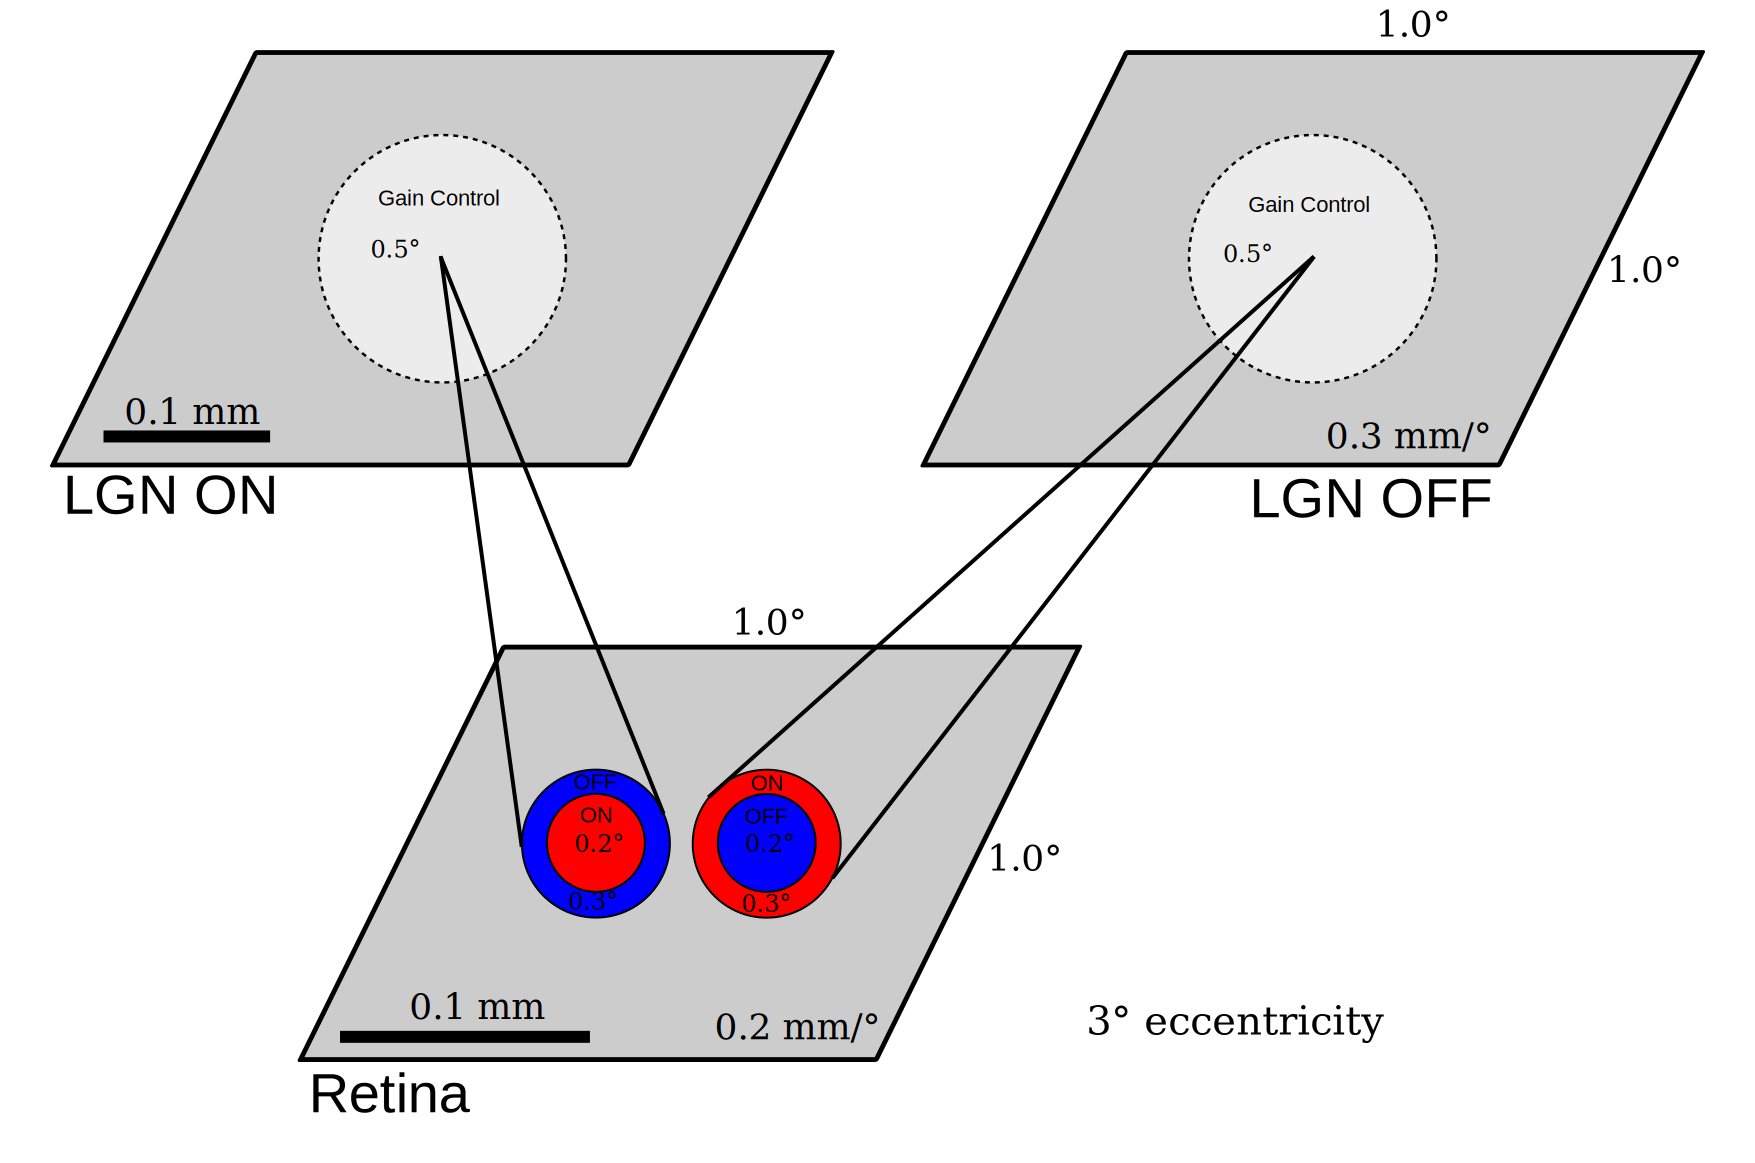
\includegraphics[width=1.0\textwidth]{LGN_Diagram.pdf}
	\caption{Diagram of the SCAL-LGN stage of the model showing
          the spatial scales of the various excitatory (red) and
          inhibitory (blue) connections. Satured colors indicate the
          kernel radii, while lightly shaded regions indicate kernel
          cut-off extents.}
	\label{LGNDiagram}
\end{figure}

\subsubsection{Input patterns}

The organization of the SOM based developmental models of the cortex,
is determined by a complex interplay between the model and the input
patterns it is trained on. Just as in the developing brain connections
are formed depending on the statistics of the sensory experience of
the strongly influencing the spatial organization of the model. In
order to accurately assess how the models respond to and self-organize
in different visual environments we will use three different visual
stimuli to present to the model.

The simplest pattern used as the baseline for most measurements will
be simply elongated Gaussian patterns matching the length of the
integrative area of a V1 neuron and with a spatial frequency that
would allow three distinct lobes to form within this area. The
training patterns are given by:

\begin{equation}
  exp(-x^2/(2*\sigma_x^2) - y^2/(2*\sigma_y^2)
\label{eqn:gausspattern}
\end{equation}

Additionally two image datasets will be employed one taken from a
database of natural images and the other recorded from within the
rearing environment of ferrets in a laboratory, which is dominated by
the long co-linear statistics of the cage bars. These datasets will
allow us to explore the effect of the natural image statistics on the
organization of the models and confirm robustness against a wide range
of visual input.

\subsubsection{Activation}

All the models operate by presenting a new retinal input at each
iteration updating the activation of each unit in each sheet. The
neurons in the sheets are firing-rate point neurons, with the main
state being a floating point activation value.  For all models, the
activation level $\eta$ for a unit at position $j$ in an ON/OFF sheet
O at time $t+\delta t$ is defined as:

\begin{equation}
\eta_{j, O}(t+\delta t)=f\left(\frac{\gamma_{O}\sum_{i\in
    F_{j,P}}\Psi_{i}(t)\omega_{ij}}{k+\gamma_{S}\sum_{i\in
    F_{j,S}}\eta_{i, O}(t)\omega_{ij, S}}\right)
\label{eqn:lgnactivation}
\end{equation}

The constant $\gamma_{O}=14.0$ is an arbitrary multiplier for the
overall strength of connections from the photoreceptor sheet to the
ON/OFF sheets, chosen to give typical activations in the range 0.0 to
1.0, while $\gamma_{S}$ is the strength of the feed-forward
contrast-gain control. $\Psi_{i}$ is the activation of unit $i$ in the
two-dimensional array of neurons on the photoreceptor sheet from which
ON/OFF unit $j$ receives input (its afferent connection field
$F_{j,P}$) and $\eta_{i, O}(t)$ is the activation of other ON/OFF
units on the previous time step (received over the suppressive
connection field $F_{j,S}$). The activation function $f$ is a
half-wave rectifying function that ensures the activation of ON/OFF
units is always positive.

The weights $\omega_{ij}$ represent the fixed connection weights from
photoreceptor $i$ to the ON or OFF unit $j$ defined with a standard
difference-of-Gaussians (DoG) kernel. The connection fields for ON units
have a positive center and negative surround, and vice versa for OFF
units. More precisely, the weight $\omega_{ij}$ from an ON-center cell
at location (0,0) in the ON sheet and a photoreceptor sheet in
location $(x,y)$ on the photoreceptor sheet is given by:

\begin{equation}
\omega_{ij}=\frac{1}{Z_c}\exp{\left(-\frac{x^{2}+y^{2}}{2\sigma_{c}^{2}}\right)}-\frac{1}{Z_s}\exp\left(-\frac{x^{2}+y^{2}}{2\sigma_{s}^{2}}\right)
\label{eqn:DoG}
\end{equation}

The kernel sizes of the central Gaussian $\sigma_{c}$ and surround
mechanism $\sigma_{s}$ are what we will be determinging here. Unlike
simple DoG kernels, the center-surround are jointly normalized to 1.0
using $Z_c$ and $Z_s$. The weights for an OFF-center cell are the
negative of the ON-center weights (i.e., surround minus center). The
center of the connection field of each ON/OFF unit is mapped to the
location in the photoreceptor sheet corresponding to the location of
that unit in sheet coordinates, making the projection retinotopic.

The weights $\omega_{ij, S}$ in the denominator of equation
\ref{eqn:lgnactivation} specify the spatial profile of the lateral
inhibition received from other ON/OFF units when contrast-gain control
is active. The weights of these connections have a fixed, circular
Gaussian profile so that for a neuron located at (0,0) in either the
ON or OFF sheet:
%%
\begin{equation}
\omega_{ij,S}=\frac{1}{Z_S}\exp\left(-\frac{x^{2}+y^{2}}{2\sigma_{S}^{2}}\right)
\label{eqn:gauss}
\end{equation}
%%
where $(x, y)$ is the location of the presynaptic neuron, $\sigma_{S}$
determines the width of the Gaussian, and $Z_S$ is a normalizing
constant that ensures that the total of all the lateral inhibitory
weights $\omega_{ij}$ to neuron $j$ sum to 1.0. This gain-control
projection is activated once per iteration before activity is sent to
the V1 sheet.

\subsubsection{The V1 model}

As we saw above in the LGN section the model described here is heavily
based on the GCAL model \citep{Stevens2013}, however it does differ in
one major respect, it employs divisive rather than subtractive
inhibition.

Each V1 neuron in each model receives connections from three different
connection types or `projections' ($p$), i.e., the afferent projection
from the ON/OFF sheets (both channels concatenated into one input
vector; $p=A$), the recurrent lateral excitatory projection ($p=E$),
and the recurrent lateral inhibitory projection ($p=I$) from other V1
neurons.

The contribution $C_{j,p}$ to the activation of unit $j$ from each
projection type ($p=A,E,I$) is calculated as:
%%
\begin{equation}
C_{j,p}(t+\delta t)=\sum_{i\in F_{j,p}}\eta_{i, p}(t)\omega_{ij,p}
\label{eqn:update}
\end{equation}
%%
where $\eta_{i, p}$ is the activation of unit $i$ taken from the set
of neurons in V1 to which unit $j$ is connected (its connection field
$F_j$) and $w_{ij,p}$ is the connection weight from unit $i$ in V1 to
unit $j$ in V1 for the projection $p$. Afferent activity ($p=A$)
remains constant after the first update from the retina, but the other
contributions change over 16 settling steps, depending on the activity
in V1.

The contributions from all three projections to V1 (afferent
($p_{A}$), excitatory $p_{E}$ and inhibitory $p_{I}$) described above
are combined using equation \ref{eqn:activation1} to calculate the
activation of a neuron $j$ in V1 at time t:
%%
\begin{equation}
\eta_{j,V}(t)=f\left(\frac{\sum_{p=\{E, A\}}\gamma_{p}C_{jp}(t)}{1+\sum_{p=\{I\}}\gamma_{p}C_{jp}(t)}\right)
\label{eqn:activation1}
\end{equation}

The projection strength scaling factors $\gamma$ are defined for each
projection type set to provide a balance between excitation and
inhibition, and between afferent and lateral influences, to provide
robust formation of activity bubbles that allows smooth maps to
form. The function $f$ defines a variable threshold point ($\theta$)
dependent on the average activity of the unit as described in the next
subsection, but in all cases the gain is fixed at unity.

At the end of the 16 settling steps, the settled V1 activation pattern
is deemed to be the V1 response to the presented pattern. At this
point we use the V1 response to update the threshold point ($\theta$)
of V1 neurons (using the adaptation process described below) and to
update the afferent and lateral inhibitory weights via Hebbian
learning. Unlike the regular GCAL model the V1 activity is not reset
to zero instead being allowed to decay until the onset of the next
visual input pattern.

\subsection*{Adaptation}

In order to set the threshold for activation, each neuron unit $j$ in
V1 calculates a smoothed exponential average of its settled activity
patterns ($\overline{\eta_{j}}$):
%%
\begin{equation}
\overline{\eta_{j}}(t)= (1-\beta)\eta_{j}(t) + \beta\overline{\eta_{j}}(t-1)
\label{eqn:averaging}
\end{equation}

The smoothing parameter ($\beta=0.991$) determines the degree of
smoothing in the calculation of the average. $\overline{\eta_{j}}$ is
initialized to the target average V1 unit activity ($\mu$), which for
all simulations is $\overline{\eta_{jA}}(0) = \mu= 0.024$. The
threshold is updated using:
%%
\begin{equation}
\label{eqn:thresholdupdate}%
\theta(t)= \theta(t-1) + \lambda(\overline{\eta_{j}}(t) -\mu)
\end{equation}
%%
where $\lambda=0.01$ is the homeostatic learning rate. The effect of
this scaling mechanism is to bring the average activity of each V1
unit closer to the specified target. If the activity in a V1 unit
moves away from the target during training, the threshold for
activation is thus automatically raised or lowered in order to bring
it closer to the target. Note that an alternative rule with only a
single smoothing parameter (rather than $\beta$ and $\lambda$) could
be formulated, but the rule as presented here makes it simple for the
modeler to set a desired target activity $\mu$.

\subsection*{Learning}

Initial connection field weights are isotropic 2D Gaussians for the
lateral excitatory projection and uniformly random within a Gaussian
envelope for afferent and lateral inhibitory
projections. Specifically, for a neuron located at (0,0):
%%
\begin{equation}
\omega_{ij}=\frac{1}{Z_p}u\exp\left(-\frac{x^{2}+y^{2}}{2\sigma_{p}^{2}}\right)
\label{eqn:gaussrandomweights}
\end{equation}
%%
where $(x, y)$ is the sheet-coordinate location of the presynaptic
neuron, $u=1$ for the lateral excitatory projection ($p=E$) and $u$ is
a scalar value drawn from a uniform random distribution for the
afferent and lateral inhibitory projections ($p=A,I$), $\sigma_{p}$
determines the width of the Gaussian in sheet coordinates
($ \sigma_{A}=0.27, \sigma_{E}=0.025, \sigma_{I}=0.075$), and $Z_p$ is
a constant normalizing term that
ensures that the total of all weights $\omega_{ij}$ to neuron $j$ in
projection $p$ is 1.0.  Weights for
each projection are only defined within a specific maximum circular
radius $r_p$ ($r_{A}=0.27, r_{E}=0.1, r_{I}=0.23$).

In the model, as images are presented to the photoreceptors, V1
afferent connection weights $\omega_{ij,A}$ from the ON/OFF sheets are
adjusted once per iteration (after V1 settling is completed) using a
simple Hebbian learning rule. This rule results in connections that
reflect correlations between the pre-synaptic ON/OFF unit activities
and the post-synaptic V1 response.  Hebbian connection weight
adjustment at each iteration is dependent on the pre-synaptic
activity, the post-synaptic response, and the Hebbian learning rate:
%%
\begin{equation}
\omega_{ij,p}(t)=\frac{\omega_{ij,p}(t-1)+\alpha\eta_{j}\eta_{i}}{\sum_{k}\left(\omega_{kj,p}(t-1)+\alpha\eta_{j}\eta_{k}\right)}
\label{eqn:hebb}
\end{equation}
%%
where for unit $j$, $\alpha$ is the Hebbian learning rate for the
afferent connection field $F_{j}$. Unless it is constrained, Hebbian
learning will lead to ever-increasing (and thus unstable) values of
the weights \citep{Rochester1956}. In all the models the weights are
constrained using divisive post-synaptic weight normalization
(equation \ref{eqn:hebb}), which is a simple and well understood
mechanism. Afferent connection weights from ON and OFF units are
normalized together in the model. We expect that a more biologically
motivated homeostatic mechanism for normalization such as
multiplicative synaptic scaling
\citep{Turrigiano1999,Turrigiano2004,Sullivan2006} or a sliding
threshold for plasticity \citep{Bienenstock1982} would achieve similar
results, but have not tested these.

The learning rates $\alpha$ are defined separately for the afferent,
lateral excitatory and lateral inhibitory projections. The
density-specific value used in the equation above is then calculated
as $\alpha=\frac{\alpha_{A}}{\tau_{A}}$, where $\tau_{A}$ is the
number of connections per connection field in the afferent projection.

\subsection{Analyses}

In order to analyse the spatial organization of the developed model we
borrow from a variety of techniques used to analyse
electrophysiological, optical imaging and anatomical data obtained in
vivo allowing us to compare directly between experimental results and
our model.

\subsubsection{Area summation curves}

The area summation curves were measured in the model by presenting the
model with disks of sine gratings of increasing size and varying phase
and at the optimal spatial frequency of each neuron. The size tuning
curves obtained in this way were then fitted with the integrated
Difference of Gaussian model described by the following equation:

\begin{equation}
R(s) = R_0 + K_e \int \int re^{-\frac{r^2}{a}} \,
\mathrm{d}r\mathrm{d}\theta - K_i \int\int re^{-\frac{r^2}{b}} \,
\mathrm{d}r\mathrm{d}\theta
\label{iDoG}
\end{equation}

\noindent where $R_0$ is the spontaneous response rate, $K_e$ the
excitatory gain, $K_i$ the inhibitory gain, $a$ the excitatory space
constant and $b$ the inhibitory space constant. By separating the
inhibitory and excitatory components in equation \ref{iDoG} and define
them as $R_e$ and $R_i$, we can formulate a subtractive and divisive
version of this equation:

\begin{equation}
R = R_e - R_i
\label{DoGSubstractive}
\end{equation}

\begin{equation}
R = \frac{R_e}{1+R_i}
\label{DoGDivisive}
\end{equation}

Using the estimated spatial constants and gain parameters we can also
calculate the suppression index of each neuron

Unlike in the original experiment we eliminate the $R_0$ and $\beta$
parameters from both models since they represent the baseline activity
and the spiking threshold respectively, which does not apply to a
firing-rate model. After fitting this model we calculate the
mean-squared error (MSE) and the explained variance of the model
($R^2$) to characterize the goodness of fit and compare how well the
two models can capture the data. Furthermore we can determine the
suppression index for the model, which is defined.

\subsubsection{Hypercolumn distance}

One of the major features of the development of the visual cortex in
higher mammals is the organization of neurons into orderly topographic
maps, forming smoothly varying feature preferences across the cortical
surface. In particular the LISSOM family of models has been able to
develop highly realistic orientation maps. These maps have been
studied in detail in various animal species and precise estimates for
their spatial scales are known. \cite{Kaschube2010} were able to
provide a detailed account of the hypercolumn distances in different
species. The hypercolumn distance is defined as the distance on the
cortical surface at which the orientation preference wraps around.

The hypercolumn distance is determined by taking the 2D fast Fourier
transform of the orientation map and collapse the real component to
1D, allowing us to determine the distance of the peak by fitting a
simple kernel to the collapsed FFT and finding the frequency of the
strongest component.

\subsubsection{Assessing the quality of orientation maps}

In addition to assessing the spatial scales in the model and comparing
them against experiment the model developed in this section should
also share other properties including robustness to a variety of
visual input, as well as smooth, robust and high-quality organization
of V1 neurons into an overall orientation map. There are a variety of
measures to assess these properties but we will focus on three in
particular, smoothness, stability and pinwheel density.

\paragraph{Pinwheel density}

Through empirical observation that orientation maps across species
share a fundamental property, that pinwheel count in biological
orientation maps scales linearly with hypercolumn size, specifically
that there are $\pi$ orientation pinwheels within the area of one
hypercolumn, when averaging over sufficiently large cortical
areas. This dimensionless, statistical measure of pinwheel
distribution is thought to reflect a universal constant of map
organization, converging to across carnivorans, primates, cats, and
tree shrews \citep{Kaschube2010, Keil2012}. This value was predicted
by a theoretical model of map organization and has strong empirical
evidence, with a mean pinwheel density across four species (tree
shrew, galago, cat, and ferret) statistically indistinguishable from
$\pi$.

To determine the pinwheel density for any given map, the hypercolumn
distance is computed and all all pinwheel centers are found. Pinwheel
centers are located at the intersection of the zero contours of the
real and imaginary components in the polar representation of
orientation preference \citep{Lowel1998}. Then we simply divide the
number of pinwheels in the modelled area by the number of hypercolumns
to arrive at the pinwheel density.

\paragraph{Stability}

The stability of orientation maps is determined by determing the
average orientation similarity index of the orientation map over the
course of development. To assess similarity quantitatively
\cite{Chapman1996} computed the correlation of orientation preference
at each developmental age with the organized preference map observed
in the final recording for that animal. As in \cite{Stevens2013} we
normalize these similarity values to fall between 0 (completely
uncorrelated) to 1 (identical orientation preference). The orientation
similarity index is therefore defined as:

\begin{equation}
  OSI = 1 - \frac{4}{n\pi} \sum_{i}\abs{(F_{i}-O_{i})mod(\frac{\pi}{2})}
\end{equation}

By averaging the OSI at every 1000 development steps we can
numerically compare the stability of the model over time. Note that
this does not provide a measure that is comparable across models
because this measure is heavily influenced by the speed of learning
but it does allow us to assess the effect of changing specific
parameters on the stability of the model.

\subsubsection{Modeling lateral connectivity}

Assessing the organization and extent of lateral connectivity in a way
that is consistent with experimental measures is difficult as they
variously use the maximum extent, which is highly dependent on the
process used for tracing the axonal projections. The only quantitively
rigorous assessment of the extent of long-range patchy connectivity in
primary visual cortex was performed by \cite{Buzas2006} in cat.

By injecting presynaptic neurons with a tracer which stains synaptic
boutons they were able to identify the location of each bouton
relative to the injected neuron and correlate it with the orientation
preference map at pre- and post-synaptic locations. This allowed them
to build a model of lateral connectivity with both spatial and
orientation dependent components, expressed as the combination of
vonMises and Gaussian distributions respectively. The orientation
dependent component is expressed as the vonMises distribution:

\begin{equation}
V(\phi, \kappa, \mu) = \frac{1}{2 \pi I_0(\kappa)} e^{\kappa cos 2(\phi - \mu)}
\end{equation}

where $\phi$ is the difference in the orientation preference between
the pre- and post-synaptic neuron, $\mu$ is the orientation preference
of the post-synaptic neuron, $\kappa$ is the concentration parameter
and $I_o(\kappa)$ is the modified Bessel function of the first kind of
zero order.

The Gaussian component on the other hand is a simple 2D Gaussian
function, where $x$ and $y$ are the cortical coordinates and $\sigma$
the SD of the Gaussian:

\begin{equation}
G(x, y, \sigma) = \frac{1}{2 \pi \sigma^2} e^{\frac{x^2+y^2}{2
    \sigma^2}}
\end{equation}

These two components can be combined into a single spatially weighted
vonMises distribution in the orientation map by simple multiplying the
components.

\begin{equation}
D_1(x, y, \phi) = s_1 [G_{11}(x, y, \sigma_{11}) V_1(\phi, \kappa_1, \mu_1)]
\end{equation}

In order to accurately estimate the local isotropic kernel an
additional Gaussian component is added, such that the full model is
described by:

\begin{equation}
D_2(x, y, \phi) = s_1 [G_{11}(x, y, \sigma_{11}) V_1(\phi, \kappa_1, \mu_1) + G_{22}(x, y, \sigma_{22})]
\end{equation}

Based on this model we can obtain estimates of the spatial extent of
the local isotropic component and separately measures of the
orientation dependence and size of the long-range lateral connectivity
kernel. We fitted this model to the long-range lateral connections in
the model using the optimization routines built into the SciPy Python
library, reporting the MSE and explained variance ($R^2$) of the final
fit when compared to a naive model ignoring the orientation dependent
component.

We further extend this model with an additional variable controlling
the aspect ratio of the long-range lateral Gaussian field relative to
the axis of preferred orientation of the pre-synaptic neuron. This
additional component allows us to capture the effect of highly
co-linear training patterns on the model connectivity.

\subsubsection{Receptive field fitting}

The receptive fields of neurons in primary visual cortex are often
described in terms of simple Gabor functions characterized by the
spatial position, phase, frequency and orientation
\citep{Jones1987,Ringach2004}. The literature also confirms that this
simple function provides a good approximation for the spatial
properties of simple cell receptive fields in the visual cortex.

The Gabor function in the real domain is defined as:

\begin{equation}
  g(x, y, \lambda, \theta, \phi, \sigma, \gamma) = exp(-\frac{x^{\prime 2} + \gamma y^{\prime 2}}{2\sigma^2}) cos(2 \pi \frac{x^\prime}{\lambda}+\phi)
\end{equation}

where

\begin{equation}
  x^\prime = x\cos(\theta) + y\sin(\theta)
\end{equation}

and

\begin{equation}
y^\prime = -x\sin(\theta) + y\cos(\theta)
\end{equation}

The spatial properties of each receptive field can be summarized by
the width of receptive field relative to frequency of the periodic
grating ($n_x$) and the elongation of the Gabor subregions relative to
the period ($n_y$). The distribution of these values, at least in
experiment, approximately follows a 1D curve indicating a shared
principle in receptive field organization that is conserved across
species.

\subsubsection{Surround modulation}

Beyond measuring simple attributes of the spatial organization in LGN
and V1, higher order effecs can be explored through complex surround
modulation measurement protocols. In addition to the simple area
summation curve measurements described above we replicate two further
protocols to evaluate the spatial response properties of the model.
In particular we are interested in the interaction between the spatial
arrangement of visual patterns presented to an animal and the contrast
on the response properties of visually responding neurons. For that
purpose we replicate two measurement protocols, a simple annulus based
contrast suppression measurement \cite{Jones2002} and a protocol using
target and flanker stimuli performed by \cite{Kapadia1995}.

\paragraph{Orientation contrast suppression}

The orientation contrast suppression is perhaps one of the most well
studied surround modulation paradigms. The measurement involves
presenting stimuli of a central sine grating, optimized to the
preferred size, frequency and orientation of the neuron being
measured. Once the baseline activity has been measured an additional
surround anulus with the same frequency is added and varied in
contrast, size and orientation to measure orientation dependent
interactions between center and surround (as shown in Figure
\ref{ORC_Stimulus}).

\begin{figure}
	\centering
        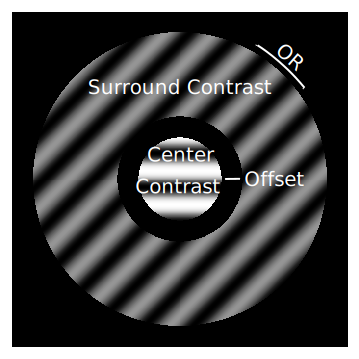
\includegraphics[width=0.5\textwidth]{ORC_Stimulus.pdf}
	\caption{Orientation contrast stimulus measuring modulation by a
      sine grating annulus on the response of a central neuron
      responding to a central sine grating disk of the same frequency.
      Stimulus is varied by center and surround contrast, surround
      orientation and the offset between the central disk and the
      surround annulus.}
	\label{ORC_Stimulus}
\end{figure}

The surround facilitation is quantified as:

\begin{equation}
F = (\frac{R_{cs}}{R_c} - 1) * 100
\end{equation}

where $R_{CS}$ is the response of the combined stimulus and $R_C$ the
response to just the center stimulus.

\paragraph{Flanker Modulation}

Instead of working solely using area based protocols we also make use
of a simple bar based stimulus along with a flanker, which is
modulated in a number of ways to characterize the surround modulation
effects associated with this protocol. In \cite{Kapadia1995} describe
a high degree of variability ranging from a complete lack of surround
modulation to facilitation and suppression. The three stimulus
protocols employed here are shown in \ref{Flanker}, we replicate these
protocol on the model to compare the effects observed in experiments
qualitatively.

\begin{figure}
	\centering
        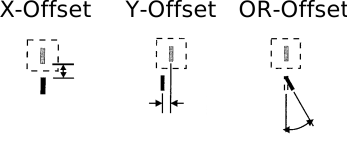
\includegraphics[width=1.0\textwidth]{FlankerProtocol.pdf}
	\caption{Flanker offset surround modulation paradigm. Measuring
      the effect of a flanker stimulus varying by an offset in X, Y
      and orientation on the response of a neuron to a target
      stimulus.}
	\label{Flanker}
\end{figure}

\section{Results}

A major component of the work in this chapter was optimizing for a
wide range of measures to achieve rough agreement with the wide range
of experimentally confirmed measurements

\subsection{Spatially calibrating LGN receptive fields}

In spatially calibrating the spatial properties of LGN receptive
fields we must take into account how they will contribute to the V1
receptive fields. One major issue in accurately modeling the LGN
connectivity is that no detailed anatomical measurements exist
describing the extent of LGN neurons and spatial measurements are
highly dependent on stimulus parameters.

In \ref{LGNTuning} we summarize population estimates from a number of
studies, measured by presenting disk masked sine gratings of varying
sizes and fitting the responses with a Difference of Gaussian model.
The estimates here vary widely with the results from
\citep{Sceniak2006} being the particular outlier. Another concern is
that it is not clear how these values translate into the existing LGN
model. To confirm this we will replicate the experimental protocols
used to obtain these values.

\begin{table}
  \centering
  \begin{adjustbox}{width=1\textwidth}
  \begin{tabular}{l | l l l l l l}
    Connection   & Literature            & Species  & Ecc. ($\degree$) & Model & Layer & $R_{c/s}$ \\
    \hline
    LGN Center   & \cite{Sceniak2006}    & macaque  & 2-5  & parvo & - & $median = 0.46 \degree$ $mean = 0.5 \degree$ \\
                 & \cite{Levitt2001}     & macaque  & 0-10 & parvo & - & $0.069 \pm 0.076 \degree$ \\
                 & \cite{Spear1994}      & macaque  & 0-10 & parvo & - & $0.087 \pm 0.046 \degree$ \\
                 & \cite{Bonin2005}      & macaque  & 13.9 & parvo & - & $0.6 \pm 0.4 \degree$\\
                 &                       &          &      &       & / & $0.4 \pm 0.2 \degree$ \\
    \hline
    LGN Surround & \cite{Sceniak2006}    & macaque  & 2-5  & parvo & - &$median = 0.51 \degree$ (0.15-0.85) \\
                 & \cite{Levitt2001}     & macaque  & 0-10 & parvo & - & $0.33 \pm 0.076 \degree$ \\
                 & \cite{Spear1994}      & macaque  & 0-10 & parvo & - & $0.53 \pm 0.39 \degree$ \\
                 & \cite{Bonin2005}      & macaque  & 13.9 & parvo & - & $2.0 \pm 1.1 \degree$\\
                 &                       &          &      &       & / & $1.8 \pm 2.6 \degree$\\

    \hline
  \end{tabular}
  \end{adjustbox}
  \caption{Estimates of LGN neuron spatial tuning properties fitted using Difference of Gaussian models
           with either subtractive or divisive suppressive components.}
  \label{LGNEstimates}
\end{table}

A set of area-summation curves measured at varying contrast levels can
be seen in Figure \ref{LGNSizeTuning}. These curves were then fitted
using the iDoG model resulting in the fit shown in Figure
\ref{LGNSizeFit}. Through an iterative process we could determine
establish a rough correspondence between the kernel sizes used in the
model definition and those obtained through the model fitting
process. However, in particular the surround size was consistently
overestimated using this procedure.

\begin{figure}
	\centering
        \includegraphics[width=1.0\textwidth]{LGN_SizeTuning.pdf}
	\caption{}
	\label{LGNSizeTuning}
\end{figure}

\begin{figure}
	\centering
        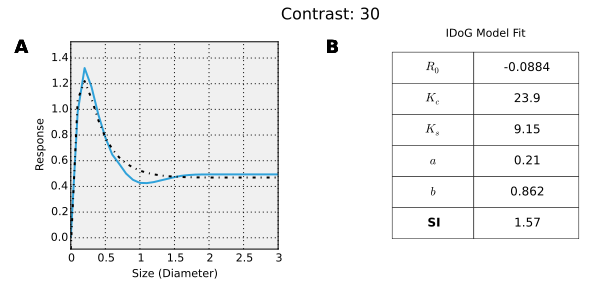
\includegraphics[width=1.0\textwidth]{LGN_SizeFit.pdf}
	\caption{A) LGN area-summation curve (blue) fit using an
          integrated Difference-of-gaussian model (dotted). B)
          Parameters of the iDoG model fit.}
	\label{LGNSizeFit}
\end{figure}

Note that neither of these models captures the mechanisms of the
SCAL-LGN model described above, which although it too operates on DoG
center-surround fields uses joint normalization and adds a distinct
divisive component, independent of the subtractive surround.

In the end it was decided that due to the large variance in results
from different studies and the limitation to a single spatial filter a
lower spatial constants should be chosen for the center-surround
mechanism. This choice allowed a fairly broad range of spatial
frequencies to be relayed to V1 to account for the lack of spatial
filter diversity. Future models should aim to cover the full
distribution of spatial frequency and size sensitivities. The final
model parameters are summarized in \ref{LGNTuning} and visualized in
Figure \ref{LGNDiagram}.
 
\begin{table}
  \centering
  \begin{adjustbox}{width=0.3\textwidth}
  \begin{tabular}{l | r}
    Model parameter   & Value \\
    \hline
    $\sigma_c$          & $0.1 \degree$  \\
    $\sigma_s$          & $0.15 \degree$ \\
    $\sigma_{gc}$        & $0.25 \degree$  \\
    $radius_{c+s}$       & $0.3 \degree$  \\
    $radius_{gc}$        & $0.5 \degree$  \\
    \hline
    $LGN_{aff}$ strength & 14 \\
    $LGN_{GC}$ strength  & 0.6 \\
  \end{tabular}
  \end{adjustbox}
  \caption{Parameters for S-patially CAL-ibrated (SCAL) LGN model.}
  \label{LGNTuning}
\end{table}

\subsection{Spatially calibrating V1 receptive fields}

A neuron in primary visual cortex receives input from a variety of
sources, including feedforward connections from the LGN, horizontal
connections from within V1 and feedback connections from extrastriate
cortex as seen in Figure \ref{Angelucci2006}. Achieving a consistent
spatial tuning is therefore a complex problems relying on a large
variety of measurements.

\begin{table}
\centering
\begin{tabular}{l | c c}
  \hline
  \hline
  Visual Area     & Magnification Factor ($mm/\deg$) & Anisotropy Index \\
  \hline
  Retina$^1$      & 0.223                            & -                      \\
  LGN$^2$         & 0.324                             & 1.0-2.0                \\
  V1$^3$          & 2.54-3.545                       & 1.0-3.0                \\
  \hline
\end{tabular}
\caption[]%
{Magnification Factors and Anisotropy Index associated with different visual areas at $3\degree$ eccentricity estimated from areal and linear magnification factor equations. Footnotes: $^1$ - \cite{Perry1985}, $^2$ - \cite{Connolly1984}, $^3$ - \cite{VanEssen1984}}
\label{MFs}
\end{table}

The first step towards a spatially calibrated model is to decide on
the region of V1 that should be targeted. Most studies of V1
particularly in the surround modulation literature focuss on parafoveal
regions between $2-5\degree$ in eccentricity. Therefore we have chosen
a region at around $3\degree$ eccentricity. This already gives us a
number of constraints, first of all gives us an approximate V1
magnification factor of 3 mm/deg as described by \cite{VanEssen1984}
and shown in Table \ref{MFs}.

Secondly to give actual scale to our model we can measure the
orientation map hypercolumn distance, which has been well established
in the literature. Using estimates provided by the Wolf group the
hypercolumn distance in macaque V1 has been estimated at roughly \(710
\pm 50 \mu m\). By combining this information with the magnification
factor we can establish that we'd expect roughly 4.2 hypercolumns per
visual degree and to keep things simple we will keep a 1:1 mapping
between visual angle and sheet coordinates of the model. We will also
define an acceptable range of hypercolumn cycles per degree to ensure
later models do not diverge too far from the spatial tuning
implemented here. Taking the confidence intervals for both the
magnification factor and hypercolumn distance into account the
acceptable range of hypercolumns per sheet coordinate is between 3.29
and 5.3.

\subsection{Methods}

The hypercolumn distance was calculated by taking the 2D Fourier
transform of the orientation map, reducing it to one dimension and
applying a least-squares fit of a Gaussian curve with additional
linear and quadratic terms (see \cite{Kaschube2010} for more
details). A sample fit to an SCAL orientation map can be seen in
Figure \ref{SCALhypercolumns}. The actual spatial calibration
procedure then was an iterative process between this hypercolumn fit
and ensuring that all the connectivity kernels matched the
experimental results outlined in the tables outlining both anatomical
results (\ref{anatomicaltable}) and electrophysiological measurements
(\ref{electrophystable}).

In particular we confirmed the spatial tuning of the afferents,
independently from the lateral connections. While electrophysiological
results were again fit using the DoG model and compared against
experimental results, the lateral connectivity was fit with a
descriptive model of the patchy, excitatory connectivity found in
layer 2/3 of the visual cortex and again compared against the
experimentally observed values.

\begin{table}
  \centering
  \begin{adjustbox}{width=1\textwidth}
  \begin{tabular}{l | l l l l}
    Connection               & Literature            & Species & Layer & $\sigma$ \\
    \hline
    LGN-V1 Afferents         & \cite{Angelucci2002c} & macaque & 4C$\alpha$ & $0.8-1.6\degree$ \\
                             & \cite{Angelucci2006a} & macaque & 4A/4C$\beta$ & $0.91 \pm 0.041 \degree$ \\
    \hline
    V1 local excitation      & \cite{Buzas2006}      & cat      & 2-4 single cell & $288 \mu m$ \\
                             & \cite{Buzas2006}      & cat      & 2-4 population  & $520 \mu m$ \\
    \hline
    V1 basket cells          & \cite{Buzas2001}      & cat      & 2-6 & $0.7-1.9 \degree$ \\
                             & \cite{Buzas2001}      & cat      & 2-6 & $0.76-2.6 mm$ \\
    \hline
    V1 long-range excitation & \cite{Angelucci2002}  & macaque  & 2/3 & $6\pm 0.7 mm$ (3-9) \\
                             &                       &          & 4B/4C$\alpha$ & $6.7 \pm 0.7 mm$ (4.7-10) \\
                             &                       &          & population & $2.47 \pm 0.3 \degree$ \\
                             & \cite{Buzas2006}      & cat      & 2/3 & $6 mm$ \\
    \hline
  \end{tabular}
  \end{adjustbox}
  \caption[]%
          {Anatomical estimates of the spatial profiles of V1 connectivity.}
  \label{anatomicaltable}
\end{table}

\begin{table}
  \centering
  \begin{adjustbox}{width=1\textwidth}
  \begin{tabular}{l | l l l l}
    Measurement              & Literature            & Species & Layer & $\sigma$ \\
    \hline
    V1 hsRF                  & \cite{Levitt2002}     & macaque & 2-6 & $1.0 \pm 0.2 \degree$ (0.3 - 2.2) \\
    \hline
    V1 Excitatory DoG fit    & \cite{Levitt2002}     & macaque & 2-6 & $0.9 \degree$ \\
                             & \cite{Sceniak2001}    & cat     & 2-6 & $1.0 \degree$ \\
                             & \cite{Cavanaugh2002}  & macaque & 2-6 & $1.4 \degree$ \\
                             & \cite{Solomon2002}    & macaque & not stated & $0.94 \degree$ \\
    \hline
    V1 Inhibitory DoG fit    & \cite{Levitt2002}     & macaque & 2-6 & $1.9 \degree$ \\
                             & \cite{Sceniak2001}    & cat     & 2-6 & $2.2 \degree$ \\
                             & \cite{Cavanaugh2002}  & macaque & 2-6 & $2.7 \degree$ \\
                             & \cite{Solomon2002}    & macaque & not stated & $2.97 \degree$ \\
    \hline
  \end{tabular}
  \end{adjustbox}
  \caption[]%
          {Functional estimates of V1 receptive field size using Difference-of-Gaussian models.}
  \label{electrophystable}
\end{table}

\begin{figure}
	\centering
        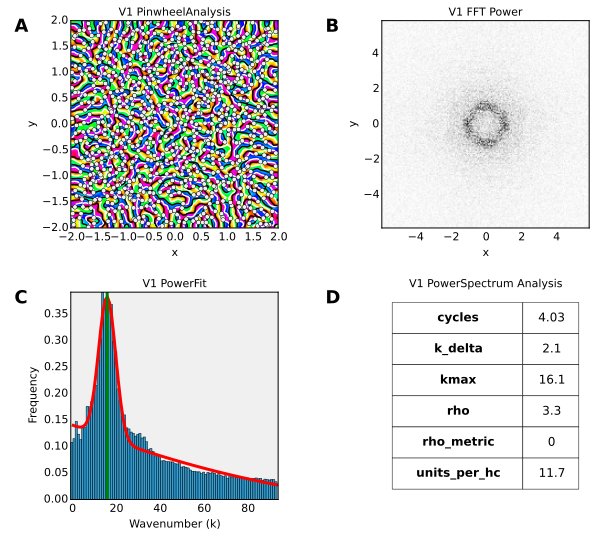
\includegraphics[width=1.0\textwidth]{SCAL_hypercolumns.pdf}
	\caption{Hypercolumn and pinwheel density fitting
          procedure. A) Orientation map in V1 overlaid with real and
          imaginary contours and pinwheels at their intersections. B)
          2D FFT of the orientation map showing a ring identifying the
          periodicity of the map. C) 1D histogram of the FFT along
          with Gaussian fit marking the best fit hypercolumn distance.
          D) Summary table showing various parameters of the fit,
          along with pinwheel density ($\rho$) which classifies the
          quality of the map.}
	\label{SCALhypercolumns}
\end{figure}

\subsection{Feedforward}

The first step in the fitting procedure was to repeat the protocols
applied to the LGN, i.e. measuring area summation curves and fitting
DoG models to the results. Using this approach we obtained a large
number of size estimates for the excitatory and inhibitory kernels
contributing to the V1 response.

\begin{figure}
	\centering
        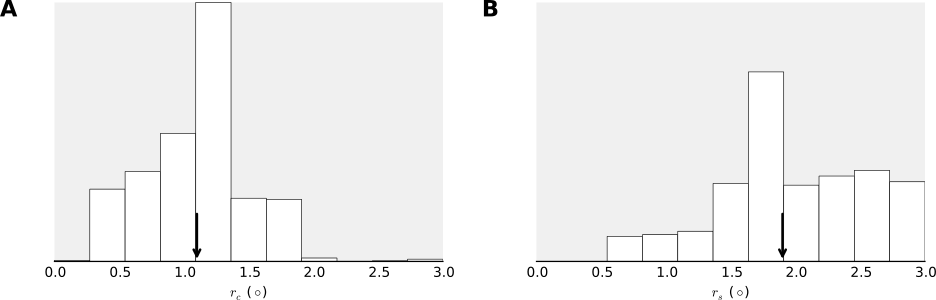
\includegraphics[width=1.0\textwidth]{SCAL_SizeDist.pdf}
	\caption{Distribution of excitatory (A) and inhibitory (B)
          Difference-of-Gaussian components fitted to area-summation
          curves measured in the SCAL V1 model. These results provide
          a close match to the results seen in Fig. 12 \& 14 of
          \cite{Sceniak2001}.}
	\label{SCALSizeDist}
\end{figure}

\subsubsection{Area summation}

Summarize table and electrophysiological results
Replicate area summation procedure
Compare distributions of fits

\subsection{Receptive Fields}

* Discuss Ringach nx/ny ratios
* Plot nx/ny plot, with overlaid fit
* Discuss circular CFs and limited filters



\subsection{Intracortical connectivity}

The intracortical connectivity can be further divided into excitatory
and inhibitory populations, we will outline the protocols for tuning
each.

\subsubsection{Excitatory Connections}

The literature has had a much harder time of picking apart the
contribution of intracortical and particularly the patchy lateral
connectivity found in V1 so to confirm that these connections have
developed as expected is to compare it to anatomical measurements.
For this purpose we will be fitting a descriptive model, developed by
\cite{Buzas2006} to the lateral connectivity data.

\begin{figure}
	\centering
        \includegraphics[width=1.0\textwidth]{Buzas.png}
	\caption{Lateral excitatory projection bouton density and
          orientation maps in layer 2/3 of cat V1 fit using a Gaussian
          and vonMises model, replicated from \cite{Buzas2006}.}
	\label{Buzas}
\end{figure}

The model describes the patchy lateral connectivity found in layer 2/3
of V1 as a function of two distinct components. A short range
isotropic Gaussian pattern and a long range pattern, defined as a von
Mises function, which is combined with the orientation map. The model
therefore assumes that lateral connectivity develops as a function of
both the proximity in space but also along a particular feature
dimension, in this case the orientation.


The full model fitting procedure for an experimentally traced lateral
connection field is shown in Figure \ref{Buzas}. By applying this
fitting procedure we can effectively estimate the spatial extents of
both the local isotropic local kernel and the long-range excitatory
kernel. In Figure \ref{SCAL_Laterals.pdf} demonstrates what one such
fit looks like for the SCAL model, while the full distribution of
local and long-range kernel values is shown in \ref{LatDist}.

The distance of long-range connectivity varies even more considerably
across species so using some anatomical estimates from macaque we will
attempt to refine our estimates of the long-range oriented
component. Anatomic data suggests that the spatial spread of lateral
connections can be anywhere between 3-10 mm (on average 6-7 mm) in
total length \cite{Angelucci2002}. Along its principal axis the
visuotopic monosynaptic spread of V1 horizontal connections has a mean
of \(2.47^\circ\) \(\pm\) \(0.3^\circ\). This falls well within the
range of estimates for the lsRF as published in a number of studies
\cite{Sceniak1999, Sceniak2001, Shushruth2009}, which employed the
iDoG protocol.

The results of our fitting procedure shown in Figure \ref{LatDist}
show good correspondence with these experimental estimates with a mean
long-range connectivity that has a spatial constant of around 5 mm but
extends beyond that with our cut-off defined at $2.5\degree$ or $7.5
mm$. The local excitatory kernel also matches experimental estimates
closely with a mean local excitatory kernel with a spatial constant of
around $350 \mu m$, compared to the $280 \mu m$ estimated in cat V1.

\begin{figure}
	\centering
        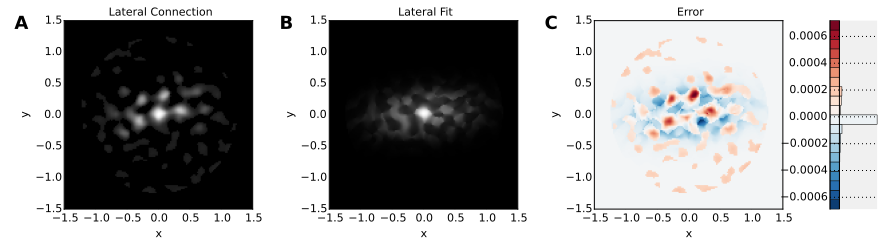
\includegraphics[width=1.0\textwidth]{SCAL_Laterals.pdf}
	\caption{Distribution of spatial constant obtained by fitting
          the \cite{Buzas2006} vonMises+Gaussian model to long-range
          lateral excitatory connections developed as part of the SCAL
          model.}
	\label{LatFits}
\end{figure}

\begin{figure}
	\centering
        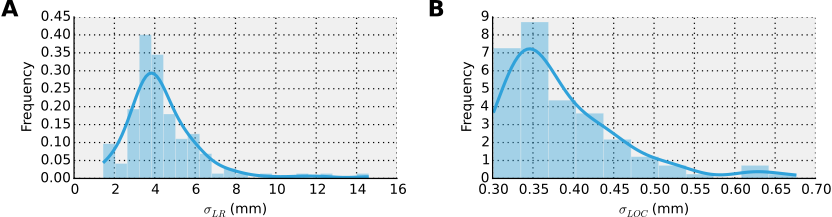
\includegraphics[width=1.0\textwidth]{SCAL_LateralFits.pdf}
	\caption{Distribution of spatial constant obtained by fitting
          the \cite{Buzas2006} vonMises+Gaussian model to long-range
          lateral excitatory connections developed as part of the SCAL
          model.}
	\label{LatDist}
\end{figure}

\subsection{Inhibitory connectivity}

The literature surrounding inhibitory connectivity is much more
limited and no good estimates of cell-type specific spatial profiles
particularly for the primate visual cortex exist. Therefore we have to
extrapolate from existing data. In the literature review we explored
the known properties of various cell classes and identified
fast-spiking Parvalbumin-expressing interneurons as the most likely
source of connectivity to drive developmental, particularly due to
their broad tuning profile and high abundance in the thalamocortical
recipient layers. Since the SCAL model does not have distinct
populations of V1 we will consider the maximal extent of known basket
cells as the maximal permitted extent of the inhibitory profile in the
model. We will revisit the spatial profiles of inhibitory connections
in the next chapter.

\subsection{Sparse connectivity}

* Real neurons only receive a few number of afferents (citation)
* We can develop sparse connectivity profiles
* Map quality does not suffer
* Show figure


\section{Conclusions}

\begin{figure}
	\centering
        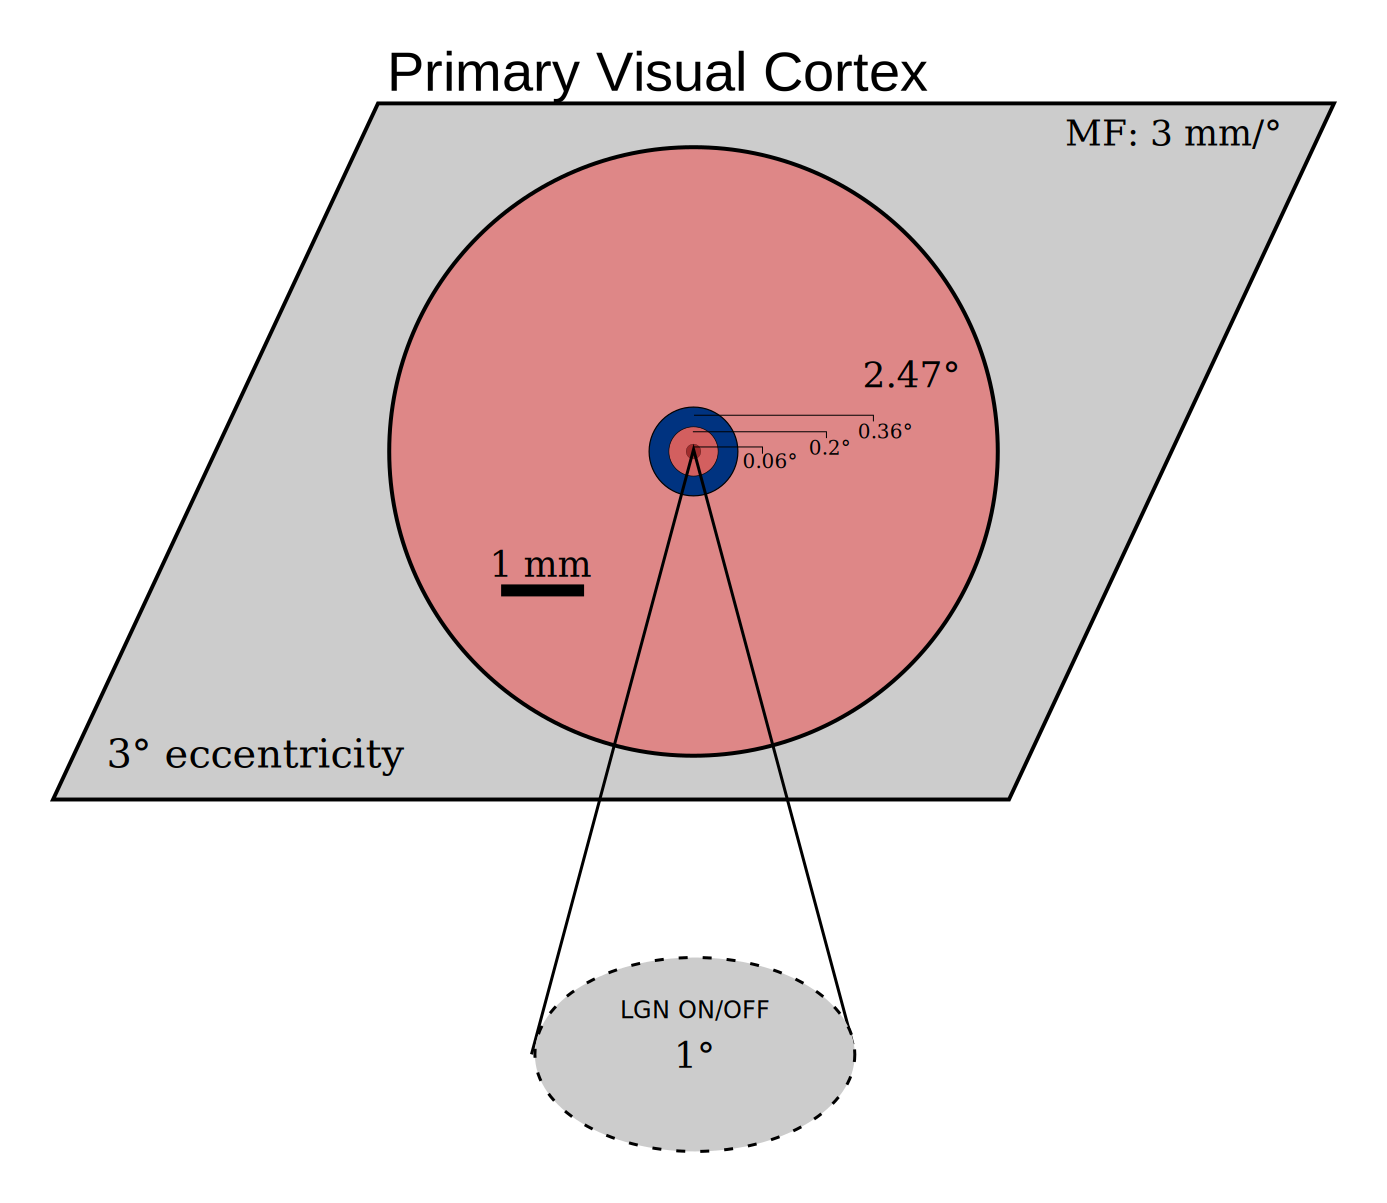
\includegraphics[width=1.0\textwidth]{SCAL_Diagram.pdf}
	\caption{Diagram of the SCAL V1 stage of the model showing
          the spatial scales of the various excitatory (red) and
          inhibitory (blue) connections. Satured colors indicate the
          kernel radii, while lightly shaded regions indicate kernel
          cut-off extents.}
	\label{SCALDiagram}
\end{figure}


To be done:

\begin{itemize}
  \item Add further plots describing the size and frequency tuning of SCAL V1.
  \item Provide further details on the lateral connectivity model fits and suggest extension based on selectivity.
  \item Optionally add analysis showing that RF nx/ny ratios closely
    follow Ringach results.
  \item Potentially add section that shows that the model can develop with realistic numbers of afferents (~30) and that lateral connectivity can be hugely sparsified (over 90\%) with little effect.
\end{itemize}
 %
%!TEX root = ../PhDthesis.tex
\chapter{Exploring the role of inhibition in cortical development}

Surround suppression is one of the most well described phenomena in
neural circuits, yet no definite conclusions on the sources of various
forms of suppressions can be drawn so far. In the literature section
of this thesis we described the known properties of various inhibitory
cell classes and what roles they might perform. In particular we
discovered that PV and SOM-expressing interneurons exhibit highly
distinct response properties and layer-specific expression patterns.
With recent techniques allowing targeting of specific populations
there is now huge interest in understanding their role both in
development and in mediating and gating the both contextual and
attentional modulation phenomena.

In this chapter we will propose models that incorporate the distinct
response properties of PV and SOM interneuron populations, allowing us
to make concrete predictions about their role in developmental and
behavioural phenomena. First we establish that the fast response and
linear response of the PV-ir, fast-spiking interneuron population
makes them ideally suited towards controlling feedforward activity,
sparsifying activity and thereby driving map formation. While
demonstrating robust and stable map formation even in the presence of
strong lateral excitation, we show that the broad tuning properties of
the PV population makes them badly suited to mediate context and
feature specific modulation. By introducing a secondary inhibitory
population modeled on the response properties of SOM+ neurons we
extend the model to demonstrate how their weaker and facilitating
inputs \citep{Bartley2008,Beierlein2003,Bartley2008,Tan2008} lead to
the development of highly tuned neurons, which respond only for high
contrasts or large stimuli, thereby mediating a range of surround
modulation phenomena.

\section{The role of inhibition in development}

Most developmental models of the primary visual cortex are based
around the concept of so called Mexican hat connectivity. This is the
idea that there is a local attractive force which pulls similar
features together and a larger repulsive force, which pushes
dissimilar features away. This is what enables the self-organization
of feature maps, which itself can be explained in terms of
dimensionality reduction, specifically forming a discretized
approximation of the principal surface of the input
\citep{Ritter1992}. In most of these models \citep{Miller1994,
  Miikkulainen2005} these interactions are modeled using point neurons
which provide excitatory and inhibitory input. In the previous chapter
we showed that an adapted version of the GCAL model
\citep{Stevens2013}, which employs divisive inhibition can still
demonstrate robust and stable map development. Here we will extend
this

\subsection{The SEPI Model}


\begin{figure}
	\centering
        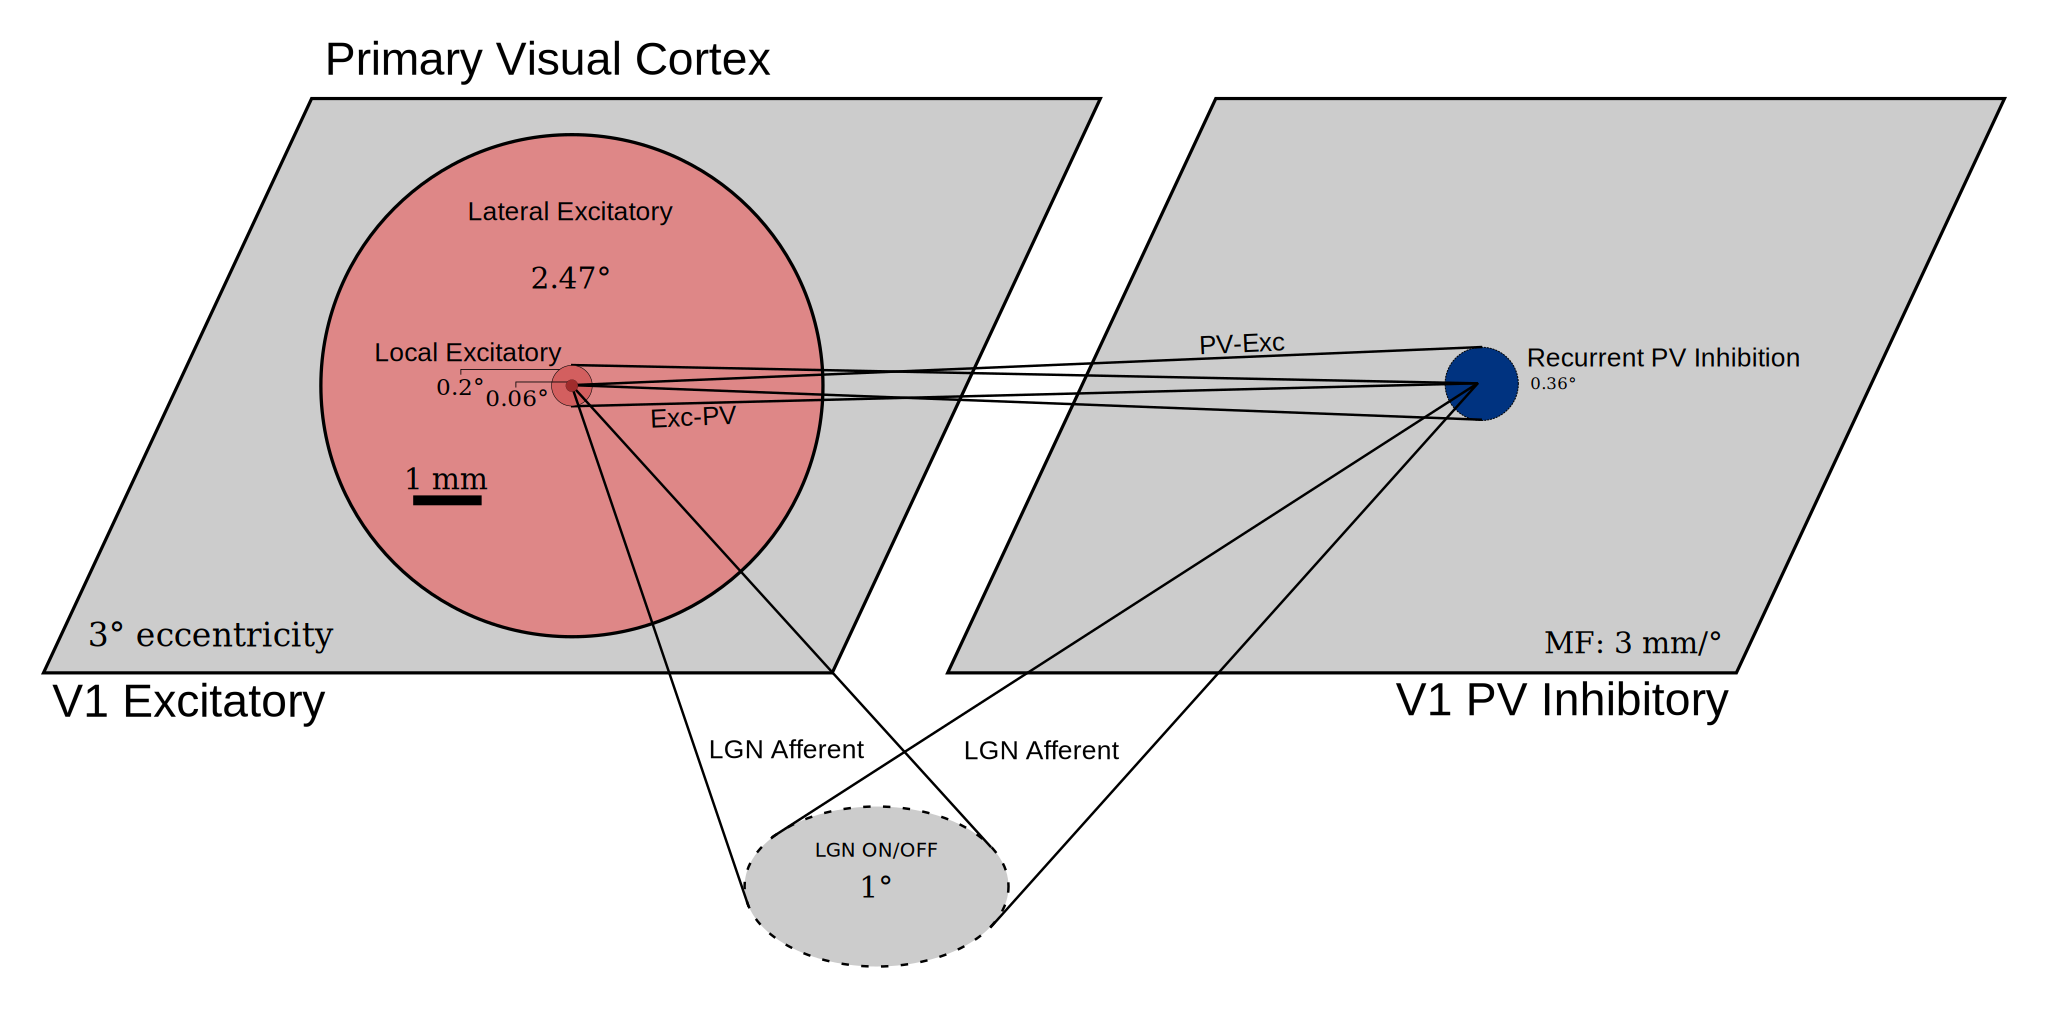
\includegraphics[width=1.0\textwidth]{SEPI_Diagram.pdf}
	\caption{Diagram of the SEPI V1 stage of the model showing the
          spatial scales of the various excitatory (red) and
          inhibitory (blue) connections. Satured colors indicate the
          kernel radii, while lightly shaded regions indicate kernel
          cut-off extents.}
	\label{SCALDiagram}
\end{figure}


\subsection{Results}

\begin{figure}
	\centering
        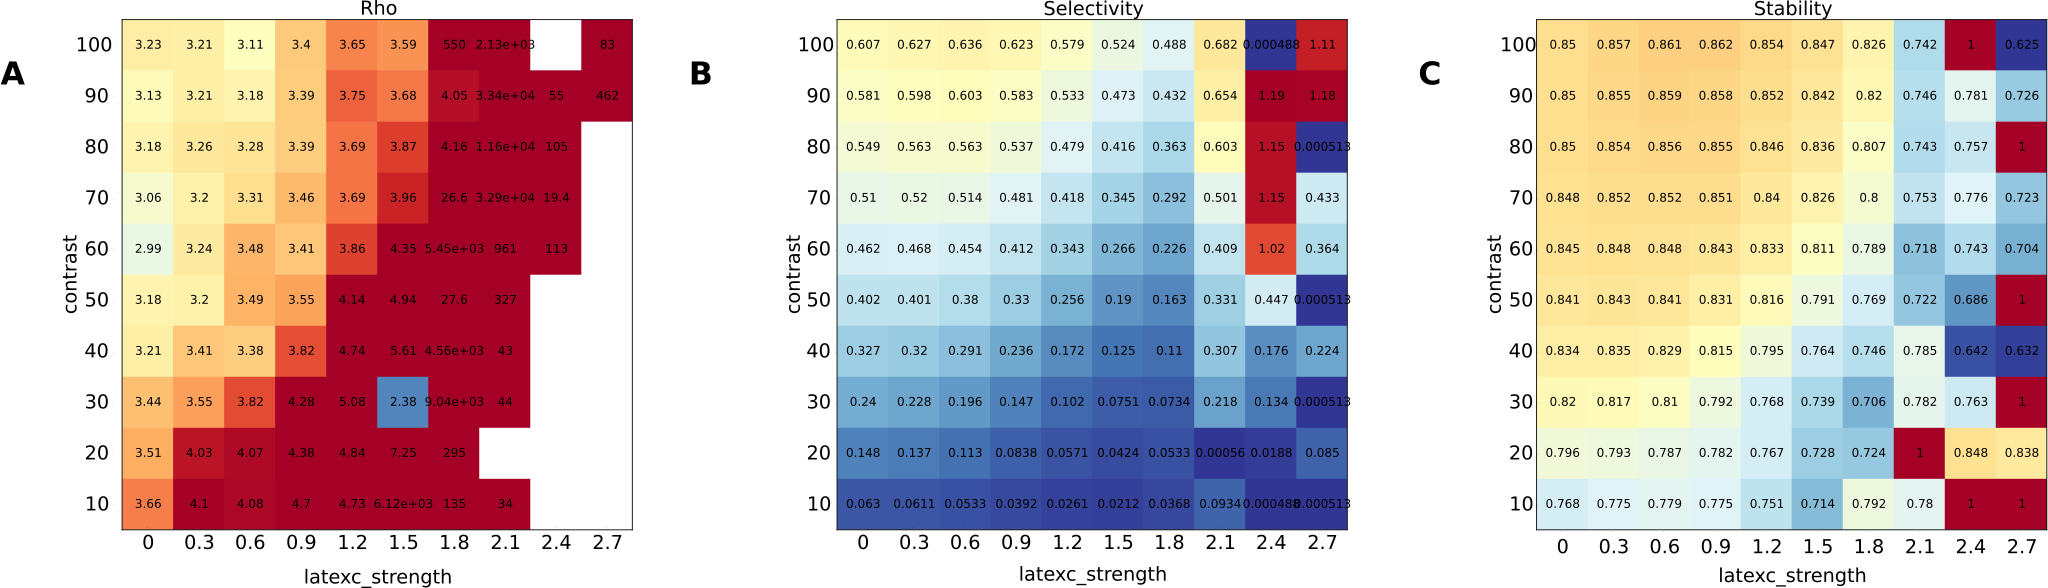
\includegraphics[width=1.0\textwidth]{SCAL_LatStability.pdf}
	\caption{Parameter explorations of three separate metrics of
          orientation map development using the SCAL model. Varied
          parameters are the strength of long-range lateral excitation
          and the stimulus contrast. The three metrics are \textbf{A}
          the $\rho$ pinwheel density metric, which characterizes the
          quality of the map, \textbf{B} the average selectivity over
          the time course of development and \textbf{C} the stability
          metric measuring how much the map changes throughout the
          course of development. The model shows good robustness to
          varying stimulus contrasts at low levels of lateral
          excitation but quickly deteriorates with increasing levels
          of excitation. White values indicate instabilities in the
          model causing the model to terminate.}
	\label{SCALStability}
\end{figure}


\begin{figure}
	\centering
        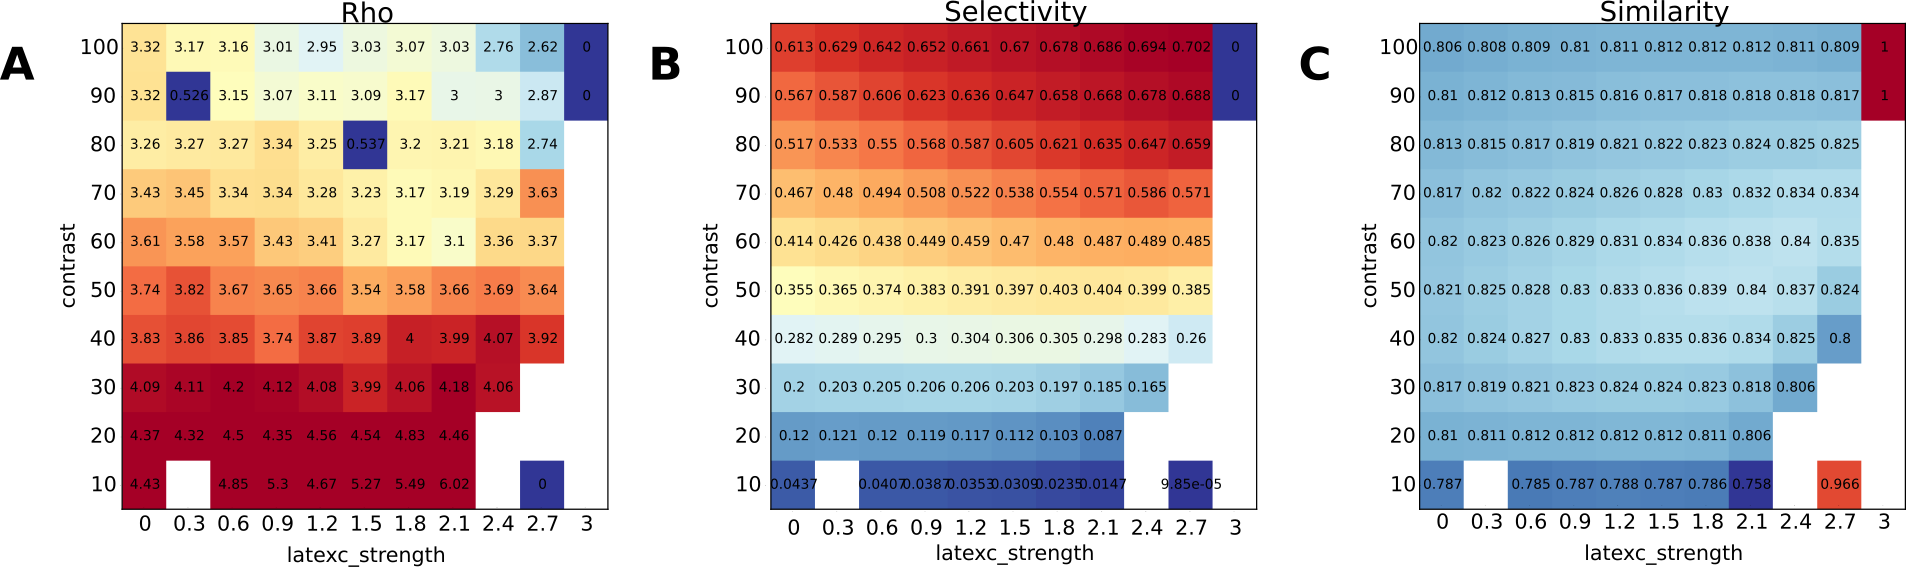
\includegraphics[width=1.0\textwidth]{SEPI_LatStability.pdf}
	\caption{Parameter explorations of three separate metrics of
          orientation map development using the SEPI model. In
          comparison to the SCAL model the pinwheel metric is not as
          robust to changes in contrast, however the model is far more
          robust to strong lateral excitation and maintains almost
          uniform stability across almost all explored parameter
          values. Uncoupling of excitation and inhibition allows the
          model to handle changes in parameter strengths but in
          absence of a homeostatic mechanism may disrupt map formation
          at low contrasts.}
	\label{SEPIStability}
\end{figure}


\section{The role of inhbition in surround modulation}


\subsection{The LESPI model}

\begin{figure}
	\centering
	\includegraphics[width=1.0\textwidth]{./v1circuit.pdf}
	\caption[]{High-level circuit diagram of the LESPI model.}
    \label{circuit_diagram}
\end{figure}


\begin{equation}
  \eta_{exc} = \frac{\eta_{A} + \eta_{LOC}}{1 + \eta_{PV}} * \eta_{SM}
\end{equation}

where $\eta_{A}$ is the LGN afferent activity, $\eta_{LOC}$ the local
excitatory contribution, $\eta_{P}$ the PV inhibitory contribution
and the surround modulation term $\eta_{SM}$ is defined as:

\begin{equation}
  \eta_{SM} = 1 + \eta_{LAT} - \eta_{S}
\end{equation}

where $\eta_{LAT}$ represents the long-range lateral excitatory
contribution and $\eta_{S}$ is the Sst inhibitory contribution. In the
SEPI model the $\eta_{SM}$ term simply reduces to 1, eliminating all
long-range interactions. The surround modulatorion term provides gain
when excitation exceeds inhibition and shunting inhibition when the
reverse is true. As such, this term provides a convenient abstraction
to model the modulatory influence of the dendritic integration of
long-range inputs.

The effective excitatory gain may not be a bad approximation to the
effect of long-range horizontal connections, which have been shown to
be strongly voltage dependent \citep{Hirsch1991}. Since Sst neurons
generally target distal dendrites they have generally been associated
with subtractive inhibition, they do however also have a
multiplicative component \citep{Wilson2012}. Additionally, their
preference for targetting distal dendrites may allow them to
effectively gate horizontal excitatory and feedback inputs
\citep{Ma2011, Gentet2012}. Additionally theoretical studies indicate
active dendritic spike backpropagation can lead to multiplicative
increases in gain, while reduction in spike backpropagation can lead
to divisive scaling of the firing rate \citep{Mehaffey2005}.
 %
%!TEX root = ../PhDthesis.tex
\chapter{Modelling the effects of visual statistics on long-range lateral connectivity in visual cortex}

One of the major problems in computational neuroscience is in
understanding how the brain can robustly capture information about its
environment to improve how new information is encoded and
processed. One of the major benefits of the developmental models such
as those developed in the previous chapters is that the developed
synaptic connections reflect the visual statistics of the
input. Therefore we can make predictions about how the statistics
embedded in the visual inputs is reflected in the organization of the
model and could be used to aid cortical computations.

A number of studies have investigated the role visual statistics play
in shaping the organization of cortex. In particular it has been shown
that the distribution of orientations in the orientation maps can be
strongly affected by altering the visual experience of an animal
through manipulations like goggle rearing \cite{Tanaka2006}. However
the evidence for the encoding of second-order statistics in lateral
connections has been much harder to study and even coarse approaches
such as measuring the isotropy of lateral connections along the axis
of preferred orientation has not yielded uniform results. While a
number of studies have found that lateral connections are elongated
along the axis of preferred orientation in tree shrew
\citep{Bosking1997}, cat \citep{Schmidt1997} and owl monkey
\citep{Sincich2001} in macaque this anisotropy could be explained by
the anisotropy in cortical magnification such that the connections are
not elongated in visual space \citep{Angelucci2002}.  Whether this
reflects differences in rearing environments or actual species
differences is not fully clear, as the tracer injections required to
reconstruct the lateral connections can be performed at most on a few
cells in a single animal, making the collection of a lot of data
infeasible.

Although there is a clear lack of data in this area a few attempts
have been made to go further and establish whether the lateral
projections connect co-circular orientation domains, relecting the
co-circularity in natural images \citep{Hunt2011}. These studies have
again been inconclusive due to the sparsity of good quality data.

In this chapter we will employ the model introduced in the previous
chapter to analyze to what extent the statistics of the visual input
shape the long-range excitatory connections and attempt to reconstruct
those statistics based purely on synaptic weights and orientation
map. In doing so we will determine to what extent they can capture the
statistics of the training dataset and establish whether considerable
biases in the inputs could affect the isotropy of connections.

\section{Methods}

\subsubsection{Synthetic stimuli} \label{synthetic}

The stimuli generated for this purpose are simple extensions of the
elongated 2D Gaussian stimuli used to train the models up to this
point. The model will draw 1 stimulus per unit area, which consists of
a chain of three Gaussian pattern, the patterns can be seen in
Figure~\ref{GaussianStatistics}. The middle Gaussian determines the
overall orientation ($\theta_M$) of the pattern, and the outer
Gaussians are offset in orientation by a value drawn from a vonMises
distribution with a mean of $\theta_M$ and a $\kappa$ of ${0.5,
  8}$. The patterns are then spatially offset so that they form a
chain forming an 'S' shape. By varying the $\kappa$ we can vary how
the distribution of co-occurence statistics increasing the preference
for simple elongated bars.

\begin{figure}
	\centering
	\includegraphics[width=1.0\textwidth]{./results/lespi/gaussian_statistics.pdf}
	\caption[Example of Gaussian patterns with co-occurence
      statistics] {Gaussian patterns with co-occurence statistics
      where the orientation offset is drawn from a vonMises
      distribution with different $\kappa$ values changing the
      distribution of orientation offsets.}
    \label{GaussianStatistics}
\end{figure}

\subsection{Co-occurence statistics}

The co-occurrence of natural image statistics have been well
characterized in a number of papers. Specifically, in a recent paper
\cite{Perrinet2015} analyzed the edge co-occurence statistics in
natural images by labeling images with edges at varying frequencies,
scales, orientations and phases through a greedy algorithm and then
computing both the relative orientation between each pair of edges and
the normalized azimuthal angle between them. An example image with
labeled edges is shown in Figure~\ref{classifier}, along with a
diagram showing how the co-occurence were computed. Similar analysis
approaches have been used to visualize the co-occurrence statistics in
natural images, such as those produced by \cite{Geisler2001} to
predict the performance of human subjects in contour detection tasks.

\begin{figure}
	\centering
    \includegraphics[width=0.8\textwidth]{./classifier.pdf}
	\caption[] {Diagramatic representation of how a classifier is
      trained to distinguish between natural images and inanimate
      objects. A) The different layers used to train the
      classifier. The natural images are first fed through a model
      retina, all the edges are labeled with positions and
      scales. Using a greedy algorithm a set of edges accounting for
      the largest amount of luminance variance within the original
      image are selected. Using this set of edges the edge
      co-occurence statistics were computed and finally the classifier
      was trained based on these statistics. B) The sparse set
      of labelled edges extracted from a single image. C) Diagram
      showing how the angular difference $\theta$ and azimuth angle
      $\phi$ and relative azimuth $\psi$ are computed from two
      edges. Reproduced from \cite{Perrinet2015}.}
	\label{classifier}
\end{figure}

The afferent receptive fields in the visual cortex are usually assumed
to act as feature detectors reducing the dimensionality of the visual
``pixel`` space into a lower dimensional representation. Connections
between these feature detectors could therefore at least in theory
represent the co-occurence statistics of the low level features. In
primary visual cortex they could therefore represents the co-occurence
of simple oriented edges. In order to test this assumption the models
were trained one various synthetic and natural image datasets and the
statistics embedded in the lateral connections were decoded.

This was done by computing the angles $\theta$, $\phi$ and $\psi$ (as
defined in figure (C) in Figure~\ref{classifier}) as well as the
euclidean distance of the receptive fields centers for each pre- and
post-synaptic pair of neurons and then binning them weighted by the
strength of connections between them. The angle $\theta$ was computed
simply as the difference between the pre- and post-synaptic neurons'
orientation preference in the orientation map and their position was
defined by computing the center of gravity of their afferent receptive
fields, allowing the angles $\phi$ and $\psi$ to be calculated. As in
previous analyses the weights were first thresholded leaving only the
strongest 10\%, ensuring that the model roughly matches the known
sparse and patchy pattern observed in anatomical tracing
studies. Additionally the neurons were selected from strong
iso-orientation regions by selecting the neurons with a local
homogeneity index above the 50th percentile. The resulting histograms
could then be further analyzed.

\subsubsection{Univariate statistics}

The simplest way to analyze these statistics was to collapse across
the dimensions to visualize the univariate distributions of the
$\theta$, $\phi$ and distance of connections. This provides an easily
understood analysis to demonstrate how strongly the connections are
biased for similar orientation, co-linear directions, an indication of
how isotropic the lateral connections are in the model and finally the
distances.

\subsubsection{Multi-variate statistics}

Using the computed histogram various plots could be generated to
compare against the plots produced by directly extracting the edge
co-occurrences from images in the \cite{Perrinet2015} and
\cite{Geisler2001} studies.

The first of these plots (Figure~\ref{SyntheticCooccurrence}), called
a Chevron map, presents the bivariate distribution of $\theta$ and
$\psi$, highlighting which spatial arrangement of edges is most likely
to co-occur. In these plots the central $1^\circ$ diameter region of
the lateral field was ignored so the plot would reflect co-occurrence
statistics of connections outside the receptive field of the
neuron. This also allowed comparing the co-occurrences between
datasets by taking the ratio of normalized weights in each bins.

The \cite{Geisler2001} type co-occurence plots on the other hand
reflect three dimensions, the angles $\theta$ and $\phi$ and the
distance, displaying the probability of an edge of a particular
orientation, co-occurring at a particular distance and azimuth
relative to the edge. It is then possible to plot the data to ask to
two related questions, (1) what is the most likely orientation of an
edge given the distance and azimuth, and (2) where is the most likely
position of an edge of a specific orientation at a specific
distance. These will be referred to as the co-circularity and
co-linearity maps respectively. \citep{Geisler2001} directly analyzed
natural image patterns for this analysis, providing a direct measure
of the statistics. In the model there is only the weights which we can
decode the statistics from. In addition to taking the weight to
compute each co-occurrence the selectivity for each orientation and
azimuth were also determined by computing the vector sum.

\subsubsection{vonMises Model}

Finally the lateral weights were again fit using the vonMises model
with both Gaussian and orientation preference dependent components,
which was first introduced in Section~\ref{BuzasEquations}. This
allows us to provide a quantitative assesment of how well the lateral
connections can be approximated with a simple model that is made up of
orientation, direction and spatially dependent components. Most
importantly the direction dependent component allows us to quantify
how strongly the lateral connection fields are biased along the axis
of preferred orientation.

\subsection{Training stimuli}

The first step was to train the model on the different image datasets,
which had already been analyzed for their co-occurence statistics
(Figure~\ref{classifier}). The datasets fed to the model comprised the
two datasets used as part of the paper and one additional image
dataset recorded in treeshrew cages in the David Fitzpatrick lab at
Duke University, which features great numbers of extended,
high-contrast bars (shown in figure \ref{image_patterns}).

\section{Results}

In order to understand the effect of different stimulus patterns on
the organization of the lateral connections both synthetic and natural
image were used. To begin with the synthetic stimulus trained model
will be analyzed to ensure the approaches work well in the simple case
and will then be extended to the natural image trained models, where a
number of issues could disrupt the model organization.

\subsection{Synthetic Stimuli}

In order to keep the analysis tractable, at least initially, a
synthetic and parameterizeable set of stimuli were used. The stimuli
described in Section \ref{synthetic} vary in both relative orientation
and azimuth, which means that if the lateral connections capture the
correlations in the inputs these correlations should also be captured
and vary depending on the width of the vonMises distributions the
orientation offsets are drawn from.

\begin{figure}
	\centering
    \includegraphics[width=1.0\textwidth]{./results/lespi/Synthetic_Distributions.pdf}
	\caption[Distributions of lateral connections of models trained on
      synthetic stimuli]{Lateral connections and histograms describing
      their orientation, azimuth and distance dependent distributions
      for narrowly and widely distributed synthetic stimuli. A, B)
      Example lateral excitatory weights after thresholding for the
      widely distributed ($\kappa=0.5$) and narrowly distributed
      ($\kappa=8$) condition. C) Orientation distribution of lateral
      connections showing stronger bias for iso-orientations in the
      narrowly distributed condition. D) Azimuth distribution showing
      strong co-linear bias for both conditions. E) Distance
      distribution showing more weight at distant locations in the
      narrowly distributed condition.}
	\label{SyntheticDistributions}
\end{figure}

By analyzing and binning the lateral weights by orientation
difference, relative azimuth and distance we can get begin to
understand what the lateral connections are actually capturing. The
difference in lateral fields between a model trained on the synthetic
stimuli with a very wide distribution ($\kappa=0.5$) and a much
tighter distribution ($\kappa=8$) is shown in
Figure~\ref{SyntheticDistributions}. This simple analysis already
makes it clear that both conditions show a strong preference for
similar orientations and co-linear stimuli, as can be seen when
looking at the azimuth histogram, which highlights a strong isotropy
along the axis of preferred orientation. This can indeed be seen even
when just looking at the sample lateral connection fields
directly. The analysis also highlights that the model trained on
patterns drawn from the tighter distribution has a slightly stronger
preference for similar orientations, and more weights at larger
distances. This reflects the stronger bias for long iso-oriented, and
co-linear contours in the input patterns.

\begin{figure}
	\centering
        \includegraphics[width=1.0\textwidth]{./results/lespi/Synthetic_Cooccurrences.pdf}
	\caption[Chevron map showing the distribution of orientation and
      azimuth differences between pre- and post-synaptic
      neurons.]{Chevron map showing the distribution of orientation
      and azimuth differences between pre- and post-synaptic neurons
      weighted by connection strength for the natural dataset (top
      left), treeshrew dataset (top right) and the difference between
      them. Modelled after \cite{Perrinet2015} co-occurrence analysis
      of natural images. Highlights the stronger bias for connecting
      iso-orientation regions in the model trained on narrowly
      distributed synthetic patterns.}
	\label{SyntheticCooccurrence}
\end{figure}

The Chevron map of edge co-occurrences, shown in
Figure~\ref{SyntheticCooccurrence}, highlights very similar trends. In
particular it demonstrates a greater spread in co-occurring
orientations as the distribution of orientation offsets in the input
pattern widens. Both the azimuth distribution and the co-occurrence
histogram also emphasize and increased preference of parallel
alignment for the tighter distribution. It is not quite clear what
drives these correlations as they are not present in the input
pattern, however through parameter exploration not shown here it was
determined that they could be reduced by presenting fewer overlapping
patterns, indicating they are artifacts.

\begin{figure}
	\centering
    \includegraphics[width=1.0\textwidth]{./results/lespi/Geisler_Synthetic_Cooccurrence.pdf}
	\caption{Co-occurrence statistics extracted from lateral
      connections to highlight the most likely orientation at each
      distance and azimuth for the two conditions (top row) and the
      most likely azimuth for each orientation and distance (bottom
      row). The colormap represents the relative probability of each
      configuration while the size reflects the selectivity for that
      particular arrangement.}
	\label{SyntheticGeisler}
\end{figure}

A further analysis using plots originally developed by
\cite{Geisler2001} demonstrates just how well the network has captured
the co-occurrence statistics of the input. The co-linearity plot
almost perfectly reflects the statistics of the input, in that the
same orientation is encountered along the axis of preferred
orientation and as we move away from this axis the preferred angle
slowly shifts away from this orientation, which is precisely how the
input pattern is defined. Additionally the model trained on the
dataset with a narrower distribution also exhibits a narrower
distribution in the co-circularity plots. This means the model has
captured not just the rough characteristics of the input but can also
capture subtler manipulations of the input. However the statistics of
the synthetic training patterns are very simplistic and capturing the
far broader distribution of visual statistics, including spatial
frequencies and spatial arrangements of patterns, that are present in
natural images is a more difficult task.

\subsection{Natural Images}

Natural and man-made environments have very different statistics,
which may be reflected in the lateral connections in the primary
visual cortex. So far we have seen that the LESPI model can indeed
capture the statistics of a simplified input pattern. Now we will a
train the model on a number of different image datasets either from
natural environments or artificial structures such as laboratory
environments. Using detailed labelling and analysis of these datasets,
which include those used by \citep{Perrinet2015} and \citep{Serre2007}
we will demonstrate that the lateral connections in V1 can already
capture the differences between different datasets, which may suggest
that they can already aid in rapid image classification based on very
low level co-occurrence statistics. Additionally we suggest that that
the rearing environment of an animal can have strong effects on the
organization of the visual system, which should be considered when
using animal models.

Man-made environments environments are characterized by co-linear,
parallel and orthogonal arrangements of edges, while true natural
images, i.e. images of natural environments, exhibit more curvature
and textured patterns \citep{Perrinet2015}. In order to test whether
the model would capture these differences a dataset three datasets
were used (1) the ``natural`` dataset containing a lot of grass
textures, (2) the ``treeshrew`` laboratory cage containing long high
contrast bars and (3) the \citep{Serre2007} target dataset of natural
scenes and animals. These represent three highly distinct visual
environments, which should be reflected in long range connections.

\subsubsection{First order statistics}

Before investigating more complex second order statistics, we analyzed
to check if partical orientations were hugely overrepresened in the
orientation map, which could introduce systematic biases to the
results. As can be seen in Figure~\ref{NatImgORs}, both dataset show
some bias for specific orientations, with the treeshrew condition
exhibiting a stronger bias along the horizontal and vertical
axes. This is likely an artifact arising from the artificial border at
the edge of the simulated sheet, which can affect the whole map
through long-range interactions.

\begin{figure}
	\centering
    \includegraphics[width=1.0\textwidth]{./results/lespi/NatImg_ORDistribution.pdf}
	\caption[Distribution of orientations in the orientation map of
      models trained on natural and laboratory images.]{Distribution
      of orientations in the orientation map of models trained on (A)
      natural and (B) laboratory images. Although all images were
      rotated to eliminate biases in the original dataset long-range
      interactions and border effects cause some biases in the model.}
	\label{NatImgORs}
\end{figure}

\subsubsection{Second order histograms}

Once again we compare the isotropy, orientation and distance
histograms between the two conditions (as shown in
Figure~\ref{NatImgDistributions}, which highlight significant
differences between the datasets. Specifically the orientation
histogram is biased much more strongly towards iso-orientations in the
natural condition. The natural condition is also considerably more
orientation selective on average, which is what drives the development
of the lateral connections. However, even though the treeshrew neurons
are a lot less selective they actually exhibit a stronger bias along
the axis of preferred orientation, with highly anisotropic lateral
connection fields. Finally we can see there is a lot more weight at
distant locations, suggesting the natural patterns exhibit more
long-range correlations overall.

\begin{figure}
	\centering
        \includegraphics[width=1.0\textwidth]{./results/lespi/NatImg_Distributions.pdf}
	\caption[Distributions of lateral weights broken down by azimuth,
      orientation and distance.]{Distributions of lateral weights
      broken down by (A) azimuth, (B) orientation and (C) distance for
      the natural and treeshrew datasets.}
	\label{NatImgDistributions}
\end{figure}

\subsubsection{Chevron Maps}

The Chevron maps offer a different view of these effects,
(Figure~\ref{NatImgCooccurrences}) as we can now see the relative
co-occurrence along both the relative azimuth and orientation
dimensions at the providing an overview of the likelihood of various
geometric arrangements. The views analyzing each dataset individually
highlight once again just how much more biased the connections are
along the $\theta$ dimension, i.e. that the connections are more
biased for similar orientations rather than specific azimuths. However
it also demonstrates that in the natural condition co-linear lines are
not much more likely than any other azimuth, which reaffirms the more
circular azimuth histogram that can be seen in
Figure~\ref{NatImgDistributions}. Comparing the distributions to ask
whether certain configurations are more likely in one dataset than the
other highlights some more interesting differences.

Specifically we can clearly see a stronger bias for parallel lines in
the natural dataset and one for orthogonal lines in the treeshrew
dataset. This may reflect the difference between textured grass
patterns with a lot of parallel arrangements and man-made structures
which exhibit far more right-angles than would usually be seen in
nature. At the same time certain curvatures are seen more strongly in
the treeshrew condition, which is surprising but may merely reflect
the lower orientation selectivity that is evident when training on
that dataset. An analysis that considers the relative orientation
independently from the azimuth may therefore shed more light on the
actual differences.

\begin{figure}
	\centering
        \includegraphics[width=1.0\textwidth]{./results/lespi/NatImg_Cooccurrences.pdf}
	\caption[Chevron map of highlighting co-occurrence statistics of
      geometrical arrangements in natural images.]{Chevron map of
      highlighting co-occurrence statistics of geometrical
      arrangements in natural images. Red indicates higher probability
      of co-occurrence, while blue indicates lower
      probability. Chevron maps for natural and treeshrew dataset
      shown on top and probability ratios comparing one dataset
      against the other below.}
	\label{NatImgCooccurrences}
\end{figure}

\subsubsection{Co-linearity and co-circularity}

Instead of considering both orientation and azimuth co-occurrences at
the same time we can treat each separately ensuring that one does not
drown out the other. The co-linearity and co-circularity plots, shown
in Figure~\ref{NatImgGeisler} alongside the results from
\cite{Geisler2001} and \cite{Perrinet2015} make these differences very
clear. Note that while the direct analysis can directly compute the
probability, the model indicates both relative probability and
confidence via the color and size respectively. Comparing just the
direct analysis to the model results for the Serre animal dataset and
the treeshrew cage dataset we can make several observations. The
treeshrew data has a much tighter distribution in the co-linearity
domain, is much more confident about the co-linearity at directions
that lie on the axis of preferred orientation, and also extends across
a much further distance. All three indicate a strong bias for
co-linear arrangements, which can also be observed in the plots
obtained directly from the datasets. However it also highlights that
decoding the azimuth from the weights adds considerable uncertainty as
the distribution is not nearly as tight as observed in experiments.

The co-circularity results also show a lot of commonalities with
almost uniformly high probability and confidence for co-circular
arrangements. However while it has assigned co-circular arrangements
very high probability in the natural condition (indicated by a bright
color) it also as assigned them low confidence indicating that
co-linear edges co-occur almost equally strongly at all azimuths. The
other striking feature about the natural condition model results is
the high confidence it has assigned to orthogonal orientations at the
axes orthogonal to the preferred orientation, even though they have
such a low overall probability. This may be driven by criss-crossing
textures such grass. Similar cross-orientation arrangements can be
observed in the Geisler results, even though it also does not assign
them very high probability. In all three model conditions the lateral
weights assign high probability to co-circular patterns however, which
is exactly what was predicted by \citep{Geisler2001}. Additionally
there is clear dataset dependent differences, which seem to match the
apparent statistics of the inputs. However there also seems to be
considerable error in decoding the relative azimuths and local
interactions, which reduce the confidence and probabilities at short
distances.

\begin{figure}
	\centering
        \includegraphics[width=1.0\textwidth]{./results/lespi/Geisler_NatImg_Cooccurrence.pdf}
	\caption{Comparison between co-linearity and co-circularity
      statistics extracted from the model and measured directly from
      the image datasets. Animals and treeshrew analyses were provided
      by Laurent Perrinet by sparsely labeling edges in the image
      datasets and computing the statistics directly and should be
      directly comparable to the corresponding model
      results. Probability is indicated through the alpha level in the
      animals/treeshrew analysis, and through color in the Geisler and
      model results. Model results additionally indicate confidence
      through the size of the edge. }
	\label{NatImgGeisler}
\end{figure}

\subsubsection{Quantifying the anisotropy}

The analyses so far have allowed us to make qualitative assessments of
how well the lateral connections in the model match the statistics in
the input patterns. In order to test whether the lateral connections
in the model are comparable to the long-range patchy connections in
layer 2/3 of V1 we will also confirm how well the lateral connections
fields are fit by the \cite{Buzas2006} model of lateral connectivity
that was introduced in \ref{BuzasEquations}. By adding the aspect
ratio of the long-range Gaussian as an additional free parameter we
can also quantitatively assess the isotropy along the axis of
preferred orientation to test our hypothesis that the anisotropy of
lateral connections observed in experiments \cite{Bosking1997} could
be explained by differences in rearing environments.

After fitting the model to all the neurons we selected the best fits
for the treeshrew and natural conditions and the error between the fit
and the actual weight pattern, allowing us to see features the model
did not capture very well. The comparison between the two fits is
shown in \ref{NatImgvonMises}. It is immediately obvious that the
treeshrew weights are considerably more elongated along the axis of
preferred orientation. The patterns of the error also highlight
several issues however, first of all it seems to assign too little
weight to the nearby iso-orientation patches, which are strongly
connected in the actual weights. Additionally there are patches that
have been assigned weight but do not have any in the actual weight
patterns. These are likely associated with phase-inversions, since the
model consists entirely of simple cells, which means that locally
iso-orientation patches with opposite phase are anti-correlated, a
feature the Buzas model does not capture.

\begin{figure}
	\centering
        \includegraphics[width=1.0\textwidth]{./results/lespi/NatImg_vonMises_Fit.pdf}
	\caption[Comparison of \cite{Buzas2006} vonMises model fit between
      the natural and treeshrew trained models.]{Comparison of
      \cite{Buzas2006} vonMises model fits between the natural and
      treeshrew trained models. A, D) Thresholded lateral fields in
      the natural and treeshrew condition. B, E) Model fitting result
      for the two conditions. C, F) Error between fitted and actual
      lateral weight fields.}
	\label{NatImgvonMises}
\end{figure}

In order to confirm that the model indeed captures the orientation
dependent component well we also let it fit the orientation directly
and confirmed the fitted orientation was well correlated with the
orientation preference in the orientation map. Overall this analysis
showed very high correlation between the estimated and measured
orientation as can be seen in Figure~\ref{NatImgvonMisesAspect}
A. Additionally we plotted the aspect ratio of the long range Gaussian
pattern against the orientation selectivity of the neurons. In the
treeshrew model the selectivity was highly correlated with the aspect,
while in the natural condition this correlation was much
weaker. Overall the mean aspect ratio for the natural condition was
1.29, while the treeshrew trained model exhibited an aspect ratio of
2.2, suggesting a much higher anisotropy along the axis of preferred
orientation.

\begin{figure}
	\centering
        \includegraphics[width=1.0\textwidth]{./results/lespi/NatImg_vonMises_aspect.pdf}
	\caption[Results from Buzas model fitting.]{Results from Buzas
      model fitting. A) Correspondence between neurons preferred
      orientation and orientation estimated based on the lateral
      connection field. B) Dependence between orientation selectivity
      and aspect ratio for the two conditions.}
	\label{NatImgvonMisesAspect}
\end{figure}

\section{Discussion}

In this chapter we explored the effect of changing the co-occurrence
statistics of the visual training on the long-range lateral
connections in a developmental model of V1 in order to test whether
various results concerning the co-circularity \citep{Hunt2011} and
anisotropy of lateral connections \citep{Bosking1997} could be
explained by differences rearing environments. Additionally we are
interested to what extent the early visual cortex is involved in
computations concerning the co-occurrence statistics to determine
whether they could be involved in computing higher order properties
such as the difference between animal and non-animal objects, which
has been shown to be computed very rapidly in human psychophysics
experiments \citep{Serre2007b}.

In performing the analysis we demonstrated that the model could
capture the statistics of simplified stimuli almost perfectly (see
Figure~\ref{SyntheticGeisler}) and demonstrated that it could even
extract the statistics of far more complex natural image stimuli to a
reasonable extent, including clear differences between various
datasets. This provides the first demonstration that a developmental
of V1 can indeed capture the statistics of natural images and can
learn various Gestalt rules for edge co-linearity and co-circularity
without hard-coding them. This suggests that encoding higher-order
statistics in the lateral connections is a general principle in the
cortex and predicts that early sensory cortices of all modalities
should capture these correlations in some way. It also highlights that
the common assumption that patchy connections in the primary visual
cortex merely link columns with similar orientation preference highly
simplistic and ignores the fact that this is simply reflects the
co-occurrence probabilities in the natural world.

Furthermore we quantify the effect of training the model in a
laboratory environment with very long, high-contrast cages and suggest
that this highly biased rearing environment will have large
implications for the organization of long-range lateral connections,
exhibiting a considerably stronger anisotropy along the axis of
preferred orientation with an anisotropy ratio of 2.2, which is
considerably higher than the anisotropy ratio of 1.29 in the model
trained on natural images. On this basis we predict that the large
anisotropy ratios observed by \citep{Bosking1997} may at least
partially explained by the rearing environment of these animals.

The novel analyses described in this chapter provide a framework to
answer questions about how higher-order correlations are captured in
the model. In future these analyses should be extended to link the
statistics encoded in the lateral connections back to the surround
modulation effects we previously showed are mediated by them. Before
such an analysis can be performed a number of issues should be
addressed.

\subsection{Spatial Frequency}

The spatial frequency distribution of natural images has been well
described in the literature as having a 1\\f
distribution. Additionally \cite{Perrinet2015} has shown that the
co-occurrence statistics are generally independent of the spatial
frequency. However the LESPI model currently only uses a single
spatial frequency filter at the level of the LGN meaning that certain
spatial frequencies are filtered out. Additionally the image patterns
used for training potentially diverge considerably from the 1\\f
distribution that has been found empirically. Indeed by investigating
the selectivity of the model trained on treeshrew images we could show
that they generally have lower spatial frequency preference than the
model trained on the natural dataset. This in turn affects the
selectivity of the model since broader spatial frequency tuning also
results in lower orientation selectivity. A future analysis should
either employ a wider range of spatial frequency filters at the LGN
level or ensure that the distribution of spatial frequency is
approximately equal across the tested datasets.

This may be particularly important because the orientation selectivity
between the models trained on the treeshrew and natural dataset
differs quite considerably, which makes comparing between them very
difficult. Specifically the Chevron maps are dominated by the
difference in orientation selectivity, which partially obscures the
the differences in azimuths.

\subsection{Complex cells and phase preference}

Another major question regarding the current analysis concerns the
fact that all the modeled neurons are simple cells by nature. As it is
known that long-range patchy connections emerge in layer 2/3, where
there is a mix of simple and complex cells this makes drawing concrete
conclusions very difficult. In particular, complex cells pool over
phase, which means they discard some of the positional information,
complicating the encoding of relative azimuth between two
edges. Extending the model to incorporate complex cells as outlined in
\cite{Antolik2010} may address some of these questions and would allow
us to make concrete predictions about the differences of lateral
connections linking simple and complex cells, which could be tested in
experiments.

Indeed the large difference in anisotropy that are observed in
treeshrews lateral connections compared to other species could reflect
the fact that layer 2/3 in treeshrews has a greater proportion of
simple cells since orientation selectivity is thought to emerge from
the connections between layer 4 and 2/3 rather than thalamocortical
projections as in other species \citep{VanHooser2013}.

\subsection{Local isotropy and suppression}

So far we have mainly discussed to what extent the connections do
reflect the statistics of the natural images the model was trained
on. There are however also clear and systematic differences which
likely reflect properties of the underlying circuit. Since the cortex
has to map high-dimensional visual features onto the 2D surface of the
cortex, there are some tradeoffs in representing all the features
perfectly. In particular since orientation is mapped onto discrete
columns the local relationships there is some distortion in the way
position is represented locally, which can be seen in some of the
co-circularity plots, which show maximal co-linear enhancement
slightly offset from the center. Additionally the local isotropic
suppression provided by the PV population will strongly suppress
cross-oriented stimuli locally, which means they do not generally show
up in the co-circularity plots as is particularly evident in the
natural condition, where they do appear at longer distances.

From a functional perspective these do not seem like major issues
since the neurons if the lateral connections are primarily concerned
with capturing co-occurrences rather than simply reflecting the
preference of the neuron in the classical receptive field. This once
again highlights the importance to consider the visuotopic extent of
lateral connections when compared to the size of the receptive
field. Depending on the species and eccentricity the neurons could
shift being primarily devoted to mediating effects within the
classical receptive field to playing a modulatory role to transmit
information from the extra-classical receptive field. Systematically
characterizing both the receptive field size and the extent of lateral
connections may therefore shed some light on their primary function.

As we concluded in the surround modulation chapter the lateral
connections in parafoveal regions of the macaque are just big enough
to mediate interactions at the borders of different textures or
between contour elements and beyond the cRF of a neuron.

\subsection{Implications for surround modulation and perception}

Having confirmed that lateral connections may be able to capture the
co-occurrence statistics of the input it is important to ask what
purpose this may serve. One of the guiding hypothesis of this thesis
and the developmental models the thesis is built on is that the
mammalian brain self-organizes based on the activity dependent
processes in order to best represent the statistics of the input. This
means that identical processes can give rise to the development of
orientation maps in visual cortex and tonotopic maps in the auditory
cortex. Rather than encoding the precise function of each brain region
the brain robustly, yet adaptively organizes in such a way that it can
optimally represent whatever input it is given. This idea is supported
by experiments performed by the Sur lab, where the retinal projection
to the LGN were rewired to the auditory thalamus and demonstrated the
animals would develop of visual receptive fields in auditory cortex
and even learn to perform various visual tasks
\citep{vonMelchner2000}.

Based on this evidence and the results presented here we argue that
the organization of the visual cortex is to a large extent an
experience dependent process and even surround modulation effects such
as contour integration and iso-orientation surround suppression are
emergent phenomena, arising because the cortex learns to represent the
visual statistics of the inputs. The role of lateral connections then
is to learn co-occurrences of the inputs expressing the model
predictions either as suppressive or facilitatory effects depending of
the geometric arrangement of the stimuli, the contrast and other
contextual information. By learning that edges in the visual
environment are generally co-linearly and co-circularly arranged even
the very earliest stages of visual processing can contribute towards
complex computations, such as detecting visually salient features
through the learned Gestalt grouping laws.

In order to predict to what extent the visual statistics of the
rearing environment affect surround modulation effects stimuli future
work should focus on generating image patterns from the input
statistics in order to see how strongly the effects can be modulated
when the statistics either match or clash with the statistics of the
rearing environment. If the statistics play a significant role then
matching the statistics should maximize the surround modulation
effects and result in a sparser representation. This may indeed be
sufficient to explain why the responses to natural images are sparser
than those for articifial stimuli.

 %
%!TEX root = ../PhDthesis.tex
\chapter{Modeling the effect of visual input statistics on surround modulation in V1}
 %
%!TEX root = ../PhDthesis.tex
\chapter{Neuromodulation of visuo-cortical information processing}
 %
%!TEX root = ../PhDthesis.tex
\chapter{General Discussion}

In this thesis we presented a series of models of the primary visual
cortex to integrate our understanding of how different cell classes
and their synaptic connections can give rise to a robust, yet dynamic
circuit to extract and encode visual features and statistics of the
world. While these models provide valuable contributions and have
allowed us to make a variety of predictions about the role of
inhibitory cell classes in development and contextual modulation, they
also simplify the full complexity in a number of crucial ways. These
simplifications have important implications about the interpretation
of the results but also offer opportunities to extend our modeling
framework.

In this discussion we will explore some of the implications of the
predictions made in the results chapters and place them into context
given our understanding of the underlying circuits. In doing so we
will.


\subsection{Spatial tuning diversity}

* Tuning diversity is limited
* Cannot capture full image statistics
* Variability in responses could affects


\subsection{Sparsity of connections}

* Afferent connections more stable
* Lateral connections more focused (+ and stable)
* Stronger surround modulation effects

\subsection{Interactions between inhibitory cells}

* PV and Sst suppress each other, Sst can disinhibit

\subsection{Complex cells}

Outline the issues with modeling only simple cells and offer
suggestions on extending the model to complex cells

* No more phase disruptions
* Loss of phase specificity for lateral connections
* Inhibition in different circuits

\subsection{Layer specific circuits}

* Clutch cells and push-pull
* PV cells for gain control
* SOM cells for spatial integration
* ViP cell modulation of lateral connections

\subsection{Neuromodulation of visuo-cortical information processing}

One of the original aims when developing the models that were
presented as part of this thesis was to develop a circuit, which would
allow for realistic modulation of specific neural subtypes and
connections. In particular the models are well suited to investigate
how the circuit can be dynamically modulated for task specific
demands, e.g. to model attentional modulation effects.

Specifically the existence of individual populations of inhibitory
neurons and a real long-range excitatory network could be used to
investigate how different neuromodulatory inputs to the cortex affect
the balance between feedforward and recurrent processing. In
particular it is hypothesized that cholinergic and adrenergic
neuromodulators are associated with attentional modulation.

\subsubsection{Cholinergic modulation}

One particular target of interest for further investigation is the
role of cholinergic inputs from the basal forebrain in mediating
attentional effects. Currently there are two main competing theories
of how cholinergic inputs to the cortex alters circuit dynamics,
outlined in the review by \cite{Thiele2013}. The first has been around
for at least two decades and suggests that cholinergic release
increases the feedforward drive and indiscriminately dis- rupts
intracortical processing. Recent evidence on the other seems to
contradict this hypothesis as a gross simplification pointing out that
different intracortical circuits are affected heterogeneously,
suggesting that while feedforward drive may be increased, layer 4
spiny cell firing is decreased, leading to weak inputs being filtered
out, while Sst-ir cell firing is also up-regulated indicating some
similarity between cholinergic modulation and the regular processing
taking place within the circuit under high contrast.

In order to test these hypothesis they could be be put to the test
through specific and well defined manipulations to the LESPI
model. The most basic manipulation would involve increasing
thalamocortical drive and reducing the strength of lateral excitatory
connections in the cortex decreased, shifting the balance of the
circuit towards feedforward processing. Additionally more specific
modulations could be applied by suppressing the Pv-ir neurons and the
Sst-ir neuron activation function steepened. Overall this should shift
the circuit towards a regime akin to the processing that occurs under
high-contrast, reducing spatial and contextual integration in favor of
more accurately representing feedforward input \citep{Roberts2005,
  Roberts2008a, Roberts2008b}.

These types of manipulations offer the chance to test various
hypothesis about how the cortical circuit can be dynamically modulated
to serve a specific task and because could even be used to model the
effect of attention on various perceptual tasks including orientation
discrimination and noisy distractor tasks.
 


%----------------------------------------------------------------------------------------
%	THESIS CONTENT - APPENDICES
%----------------------------------------------------------------------------------------

\appendix
%
%\part{Appendix} % New part of the thesis for the appendix

%%!TEX root = ../PhDthesis.tex
\chapter{Appendix}

\section{HoloViews: Building Complex Visualizations Easily for Reproducible Science} \label{SciPyPaper}

\includepdf[pages=-]{./SciPyPaper.pdf}

\section{Model Parameters} \label{Appendix:Parameters}

{\renewcommand{\arraystretch}{0.7}
\begin{tabular}{ l l l }
  \hline
	Symbol & Description & Value \\ \hline
	\ & \textbf{RGC/LGN}  & \  \\
	$\gamma_A$ & Strength of the retinogeniculate projection & 14 \\
	$\gamma_L$ & Strength of the lateral gain control & 0.6 \\
	$\sigma_C$ & Size of the center component & 0.2 \\
	$\sigma_S$ & Size of the surround component & 0.3 \\
	$\sigma_L$ & Size of the lateral gain control component & 0.25 \\
	$c$ & Constant offset of the lateral gain control function & 0.11 \\
	$\kappa_A$ & Cut-off radius of the afferent projection & 0.3 \\
	$\kappa_L$ & Cut-off radius of the lateral gain control projection & 0.5 \\
	\ & \textbf{SCAL V1}  & \  \\
	$\gamma_A$ & Strength of the geniculocortical projections & 2.4 \\
	$\gamma_E$ & Strength of the local excitatory projection & 1.6 \\
	$\gamma_I$ & Strength of the divisive inhibitory projection & 1.8 \\
	$\gamma_{LE}$ & Strength of lateral excitatory projection & 0 \\
	$\sigma_E$ & Size of local excitatory projection & 0.06 \\
	$\sigma_I$ & Size of inhibitory projection & 0.12 \\
	$\sigma_L$ & Size of lateral excitatory projection & 1.25 \\
	$\kappa_A$ & Cut-off radius of afferent projection & 0.5 \\
	$\kappa_E$ & Cut-off radius of local excitatory projection & 0.14 \\
	$\kappa_I$ & Cut-off radius of inhibitory projection & 0.18 \\
	$\kappa_L$ & Cut-off radius of lateral excitatory projection & 1.25 \\
	$\lambda_A$ & Learning-rate of the afferent projections & 0.1 \\
	$\lambda_E$ & Learning-rate of the local excitatory projection & 0 \\
	$\lambda_I$ & Learning-rate of the inhibitory projection & 0.3 \\
	$\lambda_L$ & Learning-rate of the lateral excitatory projection & 1 \\
	$\tau_L$ & Time constant of lateral projection hysteresis function & 0.2 \\
	\ & \textbf{SEPI V1 Excitatory} (Only changed)  & \  \\
	$\gamma_A$ & Strength of the afferent projection & 3 \\
	$\gamma_E$ & Strength of local excitatory projection & 2.5 \\
	$\gamma_L$ & Strength of lateral excitatory projection & 0 \\
	$\lambda_A$ & Learning-rate of the afferent projections & 0.25 \\
	$\lambda_E$ & Learning-rate of the local excitatory projection & 0 \\
	$\lambda_L$ & Learning-rate of the lateral excitatory projection & 1 \\
	\ & \textbf{SEPI V1 Parvalbumin} (Only changed)  & \  \\
	$\gamma_P$ & Strength of the divisive inhibitory projection & 2.5 \\
	$\gamma_{RP}$ & Strength of the recurrent divisive inhibitory projection & 0.8 \\
	$\lambda_P$ & Learning rate of lateral inhibitory projection & 0.25 \\
	\ & \textbf{LESPI V1 Excitatory} (Only changed) & \  \\
	$\gamma_L$ & Strength of lateral excitatory projection & 3 \\
	$\gamma_{ES}$ & Strength of local excitatory projection to Sst cells & 0.6 \\
	$\gamma_{LS}$ & Strength of lateral excitatory projection to Sst cells & 6 \\
	$\lambda_{LS}$ & Learning rate of lateral excitatory projection to Sst cells & 5 \\
	$\beta_{LS}$ & Exponent of the lateral excitatory projection to Sst cells & 3 \\
	\ & \textbf{LESPI V1 Somatostatin} & \  \\
	$\gamma_S$ & Strength of Sst inhibition projection & -1 \\
	$\tau_S$ & Time constant of Sst neuron hysteresis function & 0.2 \\
	$\lambda_S$ & Learning rate of Sst inhibition projection & 0.1 \\
\end{tabular}}
 % Appendix A
%\include{Chapters/Chapter0B} % Appendix B - empty template

%----------------------------------------------------------------------------------------
%	POST-CONTENT THESIS PAGES
%----------------------------------------------------------------------------------------

%----------------------------------------------------------------------------------------
%	List of Figures
%----------------------------------------------------------------------------------------

\refstepcounter{dummy}
\addcontentsline{toc}{chapter}{\listfigurename} % Uncomment if you would like the list of figures to appear in the table of contents
\pdfbookmark[1]{\listfigurename}{lof} % Bookmark name visible in a PDF viewer

\listoffigures

\vspace*{8ex}
\newpage

\cleardoublepage\include{FrontBackMatter/Bibliography} % Bibliography

\cleardoublepage% Colophon (a brief description of publication or production notes relevant to the edition)

\pagestyle{empty}

\hfill

\vfill

\pdfbookmark[0]{Colophon}{colophon}

\section*{Colophon}
 
\bigskip

\noindent\finalVersionString
 % Colophon


%----------------------------------------------------------------------------------------

\end{document}
